%!TEX program = xelatex
% Compile with XeLaTeX

\documentclass[10pt,professionalfonts,xcolor=table]{beamer}


%%%%%%%%%%
% Load style file, defaults  %
%%%%%%%%%%

%%%%%%%%%%%%%%%%
% Themes
%%%%%%%%%%%%%%%%

% See http://deic.uab.es/~iblanes/beamer_gallery/ for mor options

% Style theme
\usetheme{Pittsburgh}

% Color theme
\usecolortheme{lily}

% Helvetica Neue Light for most text
\usepackage[no-math]{fontspec}
\setsansfont{Helvetica Neue Light}

%%%%%%%%%%%%%%%%
% Packages
%%%%%%%%%%%%%%%%

\usepackage{geometry}
\usepackage{graphicx}
\usepackage{amssymb}
%\usepackage{epstopdf}
\usepackage{tabularx}
\usepackage{amsmath}    % this permits text in eqnarray among other benefits
\usepackage{url}    % produces hyperlinks
\usepackage[english]{babel}
\usepackage{colortbl} % allows for color usage in tables
\usepackage{multirow} % allows for rows that span multiple rows in tables
\usepackage{color}    % this package has a variety of color options
\usepackage{pgf}
\usepackage{calc}
\usepackage{ulem}
\usepackage{xspace}
\usepackage{multicol}
\usepackage{listings}
%\usepackage{changepage}
\usepackage{MnSymbol}

\usepackage{tikz}
\usepackage{fancyvrb} % for colored code chunks
\usepackage{nameref}

%%%% Flow chart $$$$
\usetikzlibrary{shapes,arrows}
\usetikzlibrary{positioning}
%%%% %%%% %%%%

%%%%%%%%%%%%%%%%
% Remove navigation symbols
%%%%%%%%%%%%%%%%

\beamertemplatenavigationsymbolsempty
\hypersetup{pdfpagemode=UseNone} % don't show bookmarks on initial view

%%%%%%%%%%%%%%%%
% User defined colors
%%%%%%%%%%%%%%%%

% Pantone 2015 Spring colors
% http://iwork3.us/2014/09/16/pantone-2015-spring-fashion-report/
% update each semester or year

\xdefinecolor{custom_blue}{rgb}{0, 0.70, 0.79} % scuba blue
\xdefinecolor{custom_darkBlue}{rgb}{0.11, 0.31, 0.54} % classic blue
\xdefinecolor{custom_orange}{rgb}{0.97, 0.57, 0.34} % tangerine
\xdefinecolor{custom_green}{rgb}{0.49, 0.81, 0.71} % lucite green
\xdefinecolor{custom_red}{RGB}{179, 51, 51}
\definecolor{emerald}{rgb}{0.13, 0.55, 0.13}
\xdefinecolor{custom_lightGray}{rgb}{0.78, 0.80, 0.80} % glacier gray
\xdefinecolor{custom_darkGray}{rgb}{0.54, 0.52, 0.53} % titanium

%%%%%%%%%%%%%%%%
% Template colors
%%%%%%%%%%%%%%%%

\setbeamercolor*{palette primary}{fg=white,bg= custom_red}
\setbeamercolor*{palette secondary}{bg=white,fg= custom_red}%!80!black}
\setbeamercolor*{palette tertiary}{bg=white,fg= custom_red}%!80!black!80}
\setbeamercolor*{palette quaternary}{bg=white,fg= custom_red}%!80!black!80}

\setbeamercolor{structure}{fg= white, bg=custom_red}
\setbeamercolor{frametitle}{bg= custom_red}
\setbeamertemplate{blocks}[shadow=false]
\setbeamersize{text margin left=1em,text margin right=1em}

%%%%%%%%%%%%%%%%
% Styling fonts, bullets, etc.
%%%%%%%%%%%%%%%%

% title slide
\setbeamerfont{title}{size=\large,series=\bfseries}
\setbeamerfont{subtitle}{size=\large,series=\mdseries}
%\setbeamerfont{institute}{size=\large,series=\mdseries}

% color of alerted text
\setbeamercolor{alerted text}{fg=custom_orange}

% styling of itemize bullets
\setbeamercolor{item}{fg=custom_red}
\setbeamertemplate{itemize item}{{{\tiny${}^\diamonddiamond$}}}
\setbeamercolor{subitem}{fg=custom_red}
\setbeamertemplate{itemize subitem}{{\tiny$ {}^\filleddiamond$}}
\setbeamerfont{itemize/enumerate subbody}{size=\footnotesize}
\setbeamerfont{itemize/enumerate subitem}{size=\footnotesize}

% styling of enumerate bullets
\setbeamertemplate{enumerate item}{\insertenumlabel.}
\setbeamerfont{enumerate item}{family={\fontspec{Helvetica Neue}}}
\setbeamerfont{enumerate subitem}{family={\fontspec{Helvetica Neue}}}
\setbeamerfont{enumerate subsubitem}{family={\fontspec{Helvetica Neue}}}

% make frame titles small to make room in the slide
\setbeamerfont{frametitle}{size=\small} 

% set Helvetica Neue font for frame and section titles
\setbeamerfont{frametitle}{family={\fontspec{Helvetica Neue}}}
\setbeamerfont{sectiontitle}{family={\fontspec{Helvetica Neue}}}
\setbeamerfont{section in toc}{family={\fontspec{Helvetica Neue}}}
\setbeamerfont{subsection in toc}{family={\fontspec{Helvetica Neue}}, size=\small}
\setbeamerfont{footline}{family={\fontspec{Helvetica Neue}}}
\setbeamerfont{subsection in toc}{family={\fontspec{Helvetica Neue}}}
\setbeamerfont{block title}{family={\fontspec{Helvetica Neue}}}

%%%%%%%%%%%%%%%%
% New fonts accessed by fontspec package
%%%%%%%%%%%%%%%%

% Monaco font for code
\newfontfamily{\monaco}{Monaco}

%%%%%%%%%%%%%%%%
% Color text commands
%%%%%%%%%%%%%%%%

%orange
\newcommand{\orange}[1]{\textcolor{custom_orange}{#1}}

% yellow
\newcommand{\yellow}[1]{\textcolor{yellow}{#1}}

% blue
\newcommand{\blue}[1]{\textcolor{blue}{#1}}

% green
\newcommand{\green}[1]{\textcolor{custom_green}{#1}}

% red
\newcommand{\red}[1]{\textcolor{custom_red}{#1}}

% dark gray
\newcommand{\darkgray}[1]{\textcolor{custom_darkGray}{#1}}

% light gray
\newcommand{\lightgray}[1]{\textcolor{custom_lightGray}{#1}}

% pink
\newcommand{\pink}[1]{\textcolor{pink}{#1}}


%%%%%%%%%%%%%%%%
% Custom commands
%%%%%%%%%%%%%%%%

% empty box for probability tree frame
\newcommand{\emptybox}[2]{
  \fbox{ \begin{minipage}{#1} \hfill\vspace{#2} \end{minipage} }
}

% cancel
\newcommand{\cancel}[1]{%
    \tikz[baseline=(tocancel.base)]{
        \node[inner sep=0pt,outer sep=0pt] (tocancel) {#1};
        \draw[red, line width=0.5mm] (tocancel.south west) -- (tocancel.north east);
    }%
}

% degree
\newcommand{\degree}{\ensuremath{^\circ}}

% cite
\newcommand{\ct}[1]{
\vfill
{\tiny #1}}

% Note
\newcommand{\Note}[1]{
\rule{2.5cm}{0.25pt} \\ \textit{\footnotesize{\textcolor{custom_red}{Note:} \textcolor{custom_darkGray}{#1}}}}

% Remember
\newcommand{\Remember}[1]{\textit{\scriptsize{\textcolor{custom_red}{Remember:} #1}}}

% links: webURL, webLink
\newcommand{\webURL}[1]{\urlstyle{same}{\textit{\textcolor{custom_red}{\url{#1}}}}}
\newcommand{\webLink}[2]{\href{#1}{\textcolor{custom_red}{{#2}}}}

% mail
\newcommand{\mail}[1]{\href{mailto:#1}{\textit{\textcolor{custom_red}{#1}}}}

% highlighting: hl, hlGr, mathhl
\newcommand{\hl}[1]{\textit{\textcolor{custom_red}{#1}}}
\newcommand{\hlGr}[1]{\textit{\textcolor{custom_red}{#1}}}
\newcommand{\mathhl}[1]{\textcolor{custom_red}{\ensuremath{#1}}}

% example
\newcommand{\ex}[1]{\textcolor{blue}{{{\small (#1)}}}}

% two col: two columns
\newenvironment{twocol}[4]{
\begin{columns}[c]
\column{#1\textwidth}
#3
\column{#2\textwidth}
#4
\end{columns}
}

% slot (for probability calculations)
\newenvironment{slot}[2]{
\begin{array}{c} 
\underline{#1} \\ 
#2
\end{array}
}

% pr: left and right parentheses
\newcommand{\pr}[1]{
\left( #1 \right)
}

%%%%%%%%%%%%%%%%
% Custom blocks
%%%%%%%%%%%%%%%%

% activity: less commonly used
\newcommand{\activity}[2]{
\setbeamertemplate{itemize item}{{{\small\textcolor{custom_orange}{$\blacktriangleright$}}}}
\setbeamercolor{block title}{fg=white, bg=custom_orange}
\setbeamerfont{block title}{size=\small}
\setbeamercolor{block body}{fg=black, bg=custom_orange!20!white!80}
\setbeamerfont{block body}{size=\small}
\begin{block}{Activity: #1}
\setlength\abovedisplayskip{0pt}
#2
\end{block}
}

% app: application exercise
\newcommand{\app}[2]{
\setbeamercolor{block title}{fg=white,bg=custom_red}
\setbeamercolor{block body}{fg=black,bg=custom_red!20!white!80}
\begin{block}{{\small Application exercise: #1}}
#2
\end{block}
}

% disc: discussion question
\newcommand{\disc}[1]{
\vspace*{-2ex}
\setbeamercolor{block body}{bg=custom_red!25!white!80, fg=custom_red!55!black!95}
\begin{block}{\vspace*{-3ex}}
#1
\end{block}
\vspace*{-1ex}
}

% clicker: clicker question
\newcommand{\clicker}[1]{
\setbeamercolor{block title}{bg=custom_red!80!white!50,fg=custom_red!30!black!90}
\setbeamercolor{block body}{bg=custom_red!20!white!80,fg=custom_red!30!black!90}
\begin{block}{\vspace*{-0.2ex}{\footnotesize Clicker question}\vspace*{-0.2ex}}
#1
\end{block}
}

% formula
\newcommand{\formula}[2]{
\setbeamercolor{block title}{bg=custom_red!40!white!60,fg=custom_red!55!black!95}
\begin{block}{{\small#1}}
#2
\end{block}
}

% code
\newcommand{\Rcode}[1]{
{\monaco {\footnotesize \textcolor{custom_darkBlue}{#1}}}
}

% output
\newcommand{\Rout}[1]{
{\monaco {\footnotesize \textcolor{custom_darkGray}{#1}}}
}

%%%%%%%%%%%%%%%%
% Change margin
%%%%%%%%%%%%%%%%

\newenvironment{changemargin}[2]{%
\begin{list}{}{%
\setlength{\topsep}{0pt}%
\setlength{\leftmargin}{#1}%
\setlength{\rightmargin}{#2}%
\setlength{\listparindent}{\parindent}%
\setlength{\itemindent}{\parindent}%
\setlength{\parsep}{\parskip}%
}%
\item}{\end{list}}

%%%%%%%%%%%%%%%%
% Footnote
%%%%%%%%%%%%%%%%

\long\def\symbolfootnote[#1]#2{\begingroup%
\def\thefootnote{\fnsymbol{footnote}}\footnote[#1]{#2}\endgroup}



%%%%%%%%%%%%%%%%
% Slide number
%%%%%%%%%%%%%%%%

%\setbeamertemplate{footline}{
%    \raisebox{5pt}{\makebox[\paperwidth]{ \makebox[200pt]{\color{gray}
%          \scriptsize \insertshortauthor woah this is a long string} \hfill\makebox[20pt]{\color{gray}
%          \scriptsize\insertframenumber/\inserttotalframenumber~}}}\hspace*{5pt}}


%\setbeamertemplate{footline}{
%  \leavevmode%
%  \hbox{%
%  \begin{beamercolorbox}[wd=.333333\paperwidth,ht=2.25ex,dp=1ex,center]{title in head/foot}%
%    \usebeamerfont{title in head/foot}\textbf{\insertshortauthor}
%  \end{beamercolorbox}%
%  \begin{beamercolorbox}[wd=.333333\paperwidth,ht=2.25ex,dp=1ex,center]{title in head/foot}%
%    \usebeamerfont{title in head/foot}\textbf{\insertshorttitle}
%  \end{beamercolorbox}%
%  \begin{beamercolorbox}[wd=.333333\paperwidth,ht=2.25ex,dp=1ex,right]{date in head/foot}%
%    \usebeamerfont{date in head/foot}\textbf{\insertshortdate{}\hspace*{2em}
%    \insertframenumber{} / \inserttotalframenumber\hspace*{2ex} }
%  \end{beamercolorbox}}%
%  \vskip0pt%
%}

\setbeamertemplate{footline}{
  \leavevmode%
  \hbox{%
  \begin{beamercolorbox}[wd=.7\paperwidth,ht=2.25ex,dp=1ex,left]{title in head/foot}%
    \usebeamerfont{title in head/foot}\textbf{\hspace*{2ex}\insertshorttitle~(\insertshortauthor)}
  \end{beamercolorbox}%
  \begin{beamercolorbox}[wd=.3\paperwidth,ht=2.25ex,dp=1ex,right]{date in head/foot}%
    \usebeamerfont{date in head/foot}\textbf{\insertshortdate{}\hspace*{2em}
    \insertframenumber{} / \inserttotalframenumber\hspace*{2ex} }
  \end{beamercolorbox}}%
  \vskip0pt%
}

%%%%%%%%%%%%%%%%
% Remove page numbers
%%%%%%%%%%%%%%%%

%\newcommand{\removepagenumbers}{%
%  \setbeamertemplate{footline}{}
%}

\newcommand{\bang}{\item[\tiny${}^\diamonddiamond$]}
\newcommand{\bing}{\item[\tiny${}^\filleddiamond$]}
\newcommand{\bong}{\item[~]}
\newcommand{\bangon}{\begin{itemize}}
\newcommand{\bangoff}{\end{itemize}}
\newcommand{\numu}{$\nu_\mu$\xspace}
\newcommand{\nue}{$\nu_e$\xspace}
\newcommand{\nova}{NO$\nu$A\xspace}
\newcommand{\gap}{\vspace{10pt}}


%%%%%%%%%%%%%%%%
% TOC slides
%%%%%%%%%%%%%%%%

\setbeamertemplate{section in toc}{\inserttocsectionnumber.~\inserttocsection}
\setbeamertemplate{subsection in toc}{$\qquad$\inserttocsubsectionnumber.~\inserttocsubsection \\}

\AtBeginSection[] 
{ 
  \addtocounter{framenumber}{-1} 
  % 
  {\removepagenumbers 
  {\small
    \begin{frame}<beamer> 
    \frametitle{Outline} 
    \tableofcontents[currentsection] 
  \end{frame} 
  } 
  }
} 

\AtBeginSubsection[] 
{ 
  \addtocounter{framenumber}{-1} 
  % 
  {\removepagenumbers 
  {\small
    \begin{frame}<beamer> 
    \frametitle{Outline} 
    \tableofcontents[currentsection,currentsubsection] 
  \end{frame} 
  } 
  }
}




%%%%%%%%%%%
% Cover slide info    %
%%%%%%%%%%%
%\setbeamertemplate{sections/subsections in toc}[sections numbered]

\title[\numu Disappearance CNN]{Muon Neutrino Disappearance in NOvA with a Deep Convolutional Neural Network Classifier}
\author[D. Rocco]{Dominick Rocco}
\date{\today}
\institute{University of Minnesota}

\begin{document}

\tikzstyle{block} = [rectangle, draw, fill=cyan!40,
   text width=3.25cm, text centered, rounded corners, minimum height=4em, minimum width = 3cm]
\tikzstyle{line}=[draw, ->, thick]
\tikzstyle{lin}=[draw, -, thick]
\tikzstyle{dot} = [minimum size=0.00pt,inner sep=0pt]
\tikzstyle{cloud} = [draw, ellipse,fill=red!50, node distance=3cm,
   minimum height=2em]

\frame{\titlepage}


\begin{frame}
\app{Neutrino (\textit{noun})}{An abundant particle which rarely interacts \\
\gap
e.g. \textit{Neutrinos are everywhere in the universe, billions of them are currently passing through this room undetected.}}
\end{frame}



\frame
{
  \frametitle{Standard Model of Particle Physics}

\begin{columns}[c]
\column{0.6\textwidth}
  \begin{itemize}
  \bang The standard model enumerates fundamental particles
  \bang Fundamental: not comprised of other particles

  \bang \textbf{Quarks}:
    \begin{itemize}
    \bing Make up protons and neutrons...
    \bong ... and pions ($\pi$) and kaons ($K$)
    \bong ... and much much more woah

    \end{itemize}
  \bang \textbf{Leptons}:
    \begin{itemize}
    \bing Include electron ($e$) and heavier cousins muon ($\mu$) and ($\tau$)
    \bing Also includes a neutrino to compliment each one
    \end{itemize}
  \bang \textbf{Bosons}:
    \begin{itemize}
    \bing Force carriers -- mediate interactions between other particles
    \end{itemize}

  \end{itemize}
\column{0.5\textwidth}
    \begin{figure}
  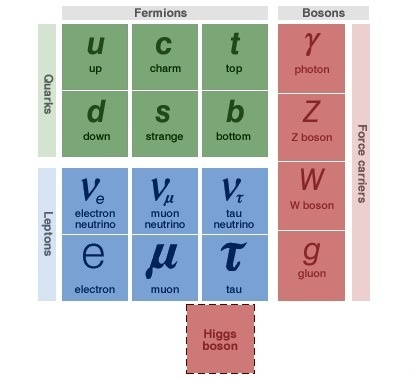
\includegraphics[width=\textwidth]{figures/figures/stdmod.jpg}
  \end{figure}
\end{columns}

}


\begin{frame}
  \frametitle{Neutrino Interactions}

  \begin{itemize}
  \bang Neutrinos are very small
    \begin{itemize}
    \bing ... i.e. they rarely interact with ordinary matter
    \bing Neutral to both electromagnetic and strong forces
    \bing Billions of them are passing through you right now without interacting
    \bing Could travel through a light-year of lead and probably not interact
    \end{itemize}
    \end{itemize}
    \gap
    \begin{columns}
      \column{0.5\textwidth}
  \centering
  \textcolor{custom_red}{Charged Current}


  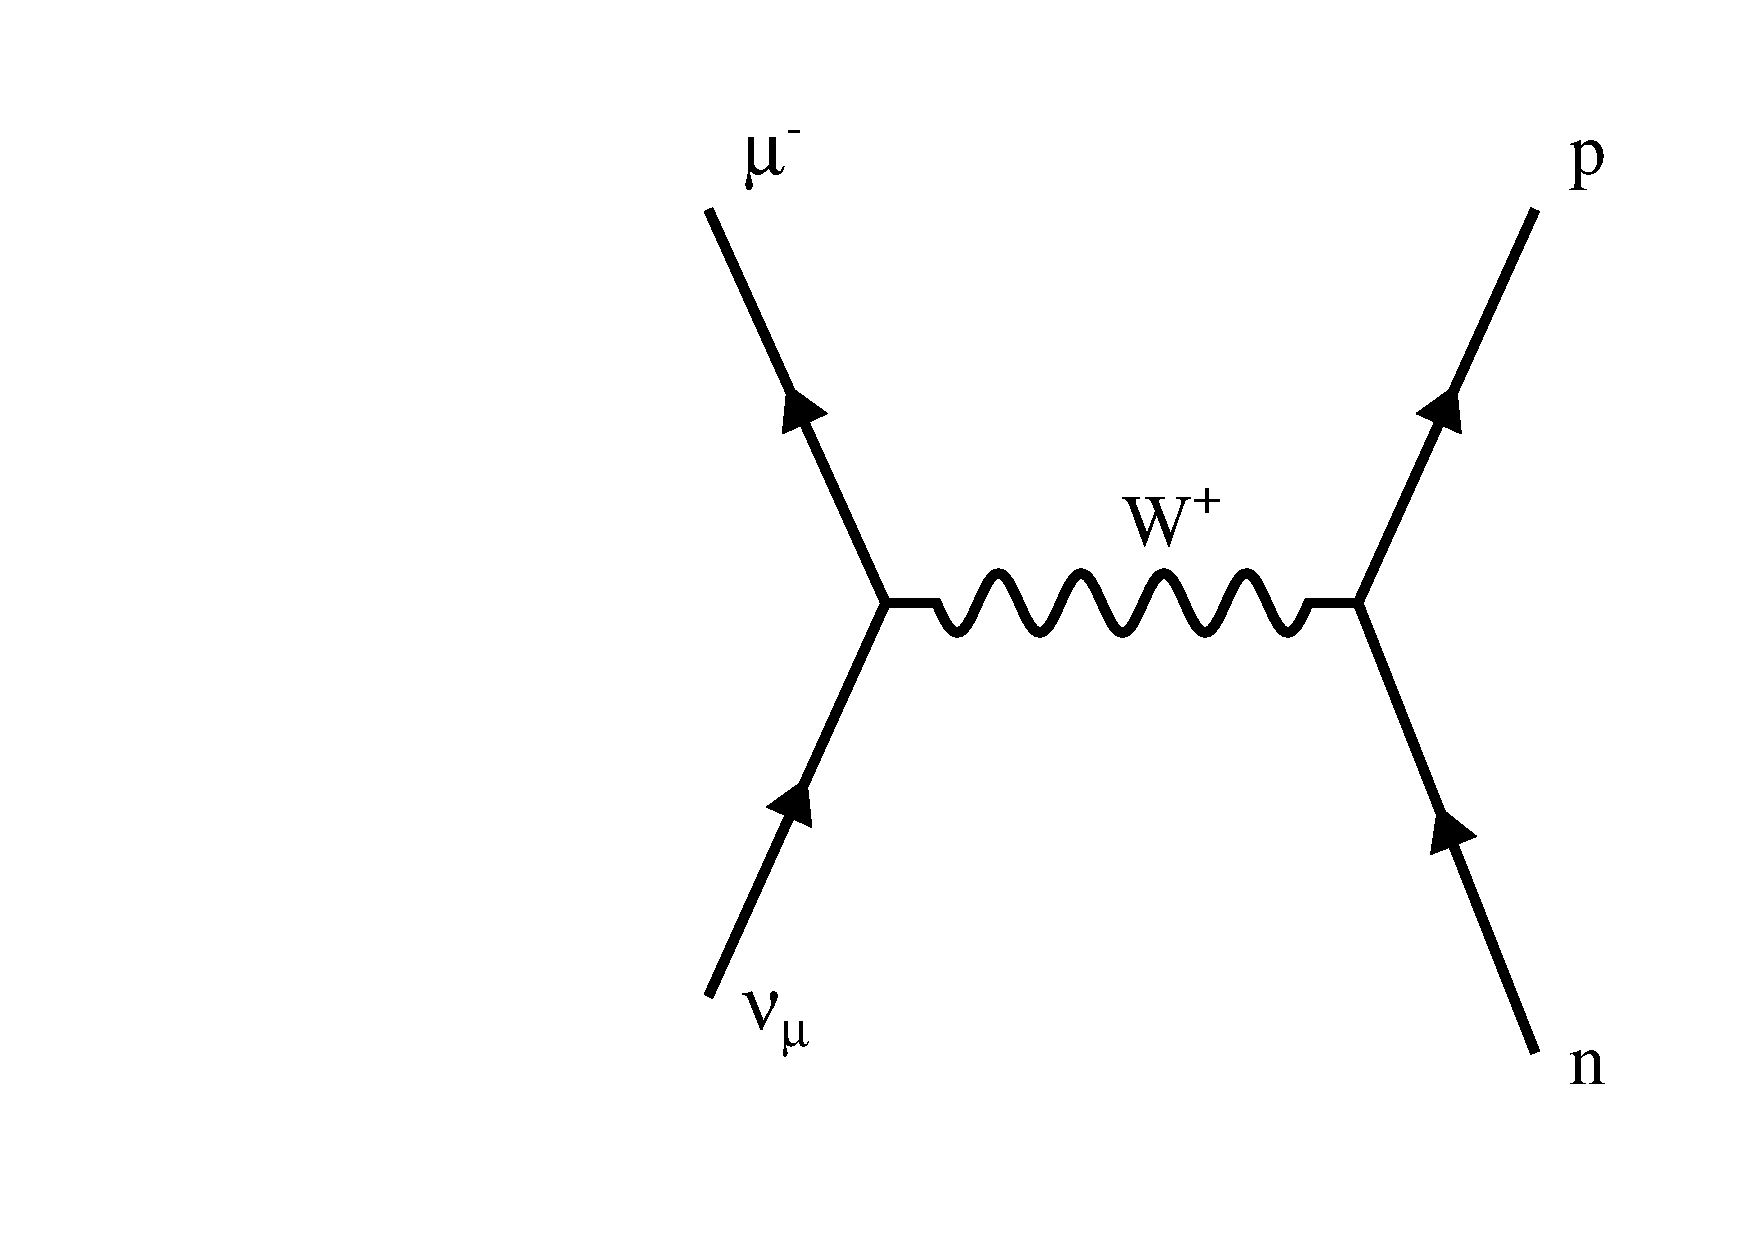
\includegraphics[height=0.37\textheight, angle=-90]{figures/feynman/ccNumu.pdf}
  \column{0.5\textwidth}
  \centering
   \textcolor{custom_red}{Neutral Current}


  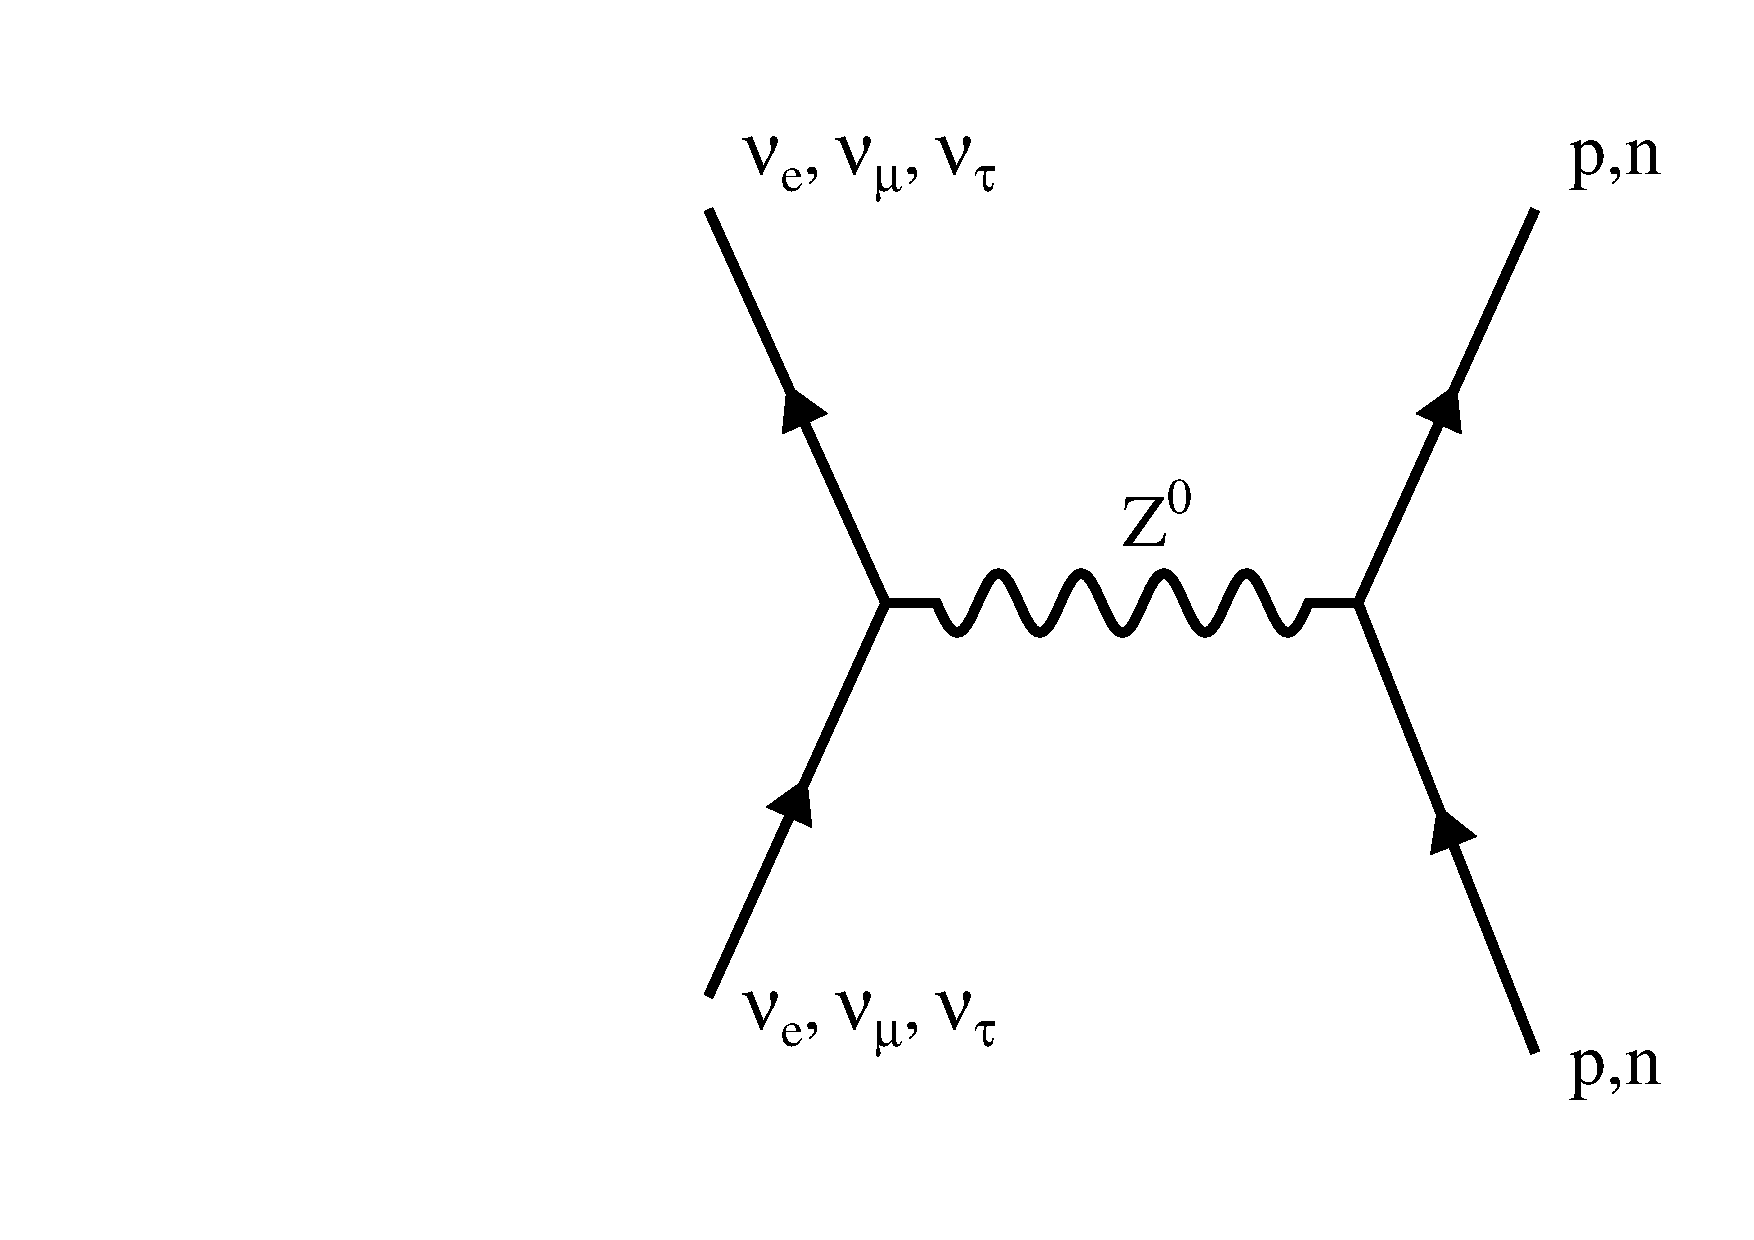
\includegraphics[height=0.37\textheight, angle=-90]{figures/feynman/ncHad.pdf}
  \end{columns}
\gap
    \begin{itemize}
    \item Weak interactions involve either $W$ or $Z$ bozon
      \begin{itemize}
      \item $W$: charged current
      \bong ~~~~ $\nu_e \rightarrow e$ ~~ or ~~ $\nu_\mu \rightarrow \mu$ ~~ or ~~ $\nu_\tau \rightarrow \tau$
      \item $Z$: neutral current
      \bong ~~~~ $\nu_e \rightarrow \nu_e$ ~~ or ~~ $\nu_\mu \rightarrow \nu_\mu$ ~~ or ~~ $\nu_\tau \rightarrow \nu_\tau$
      \end{itemize}
    \end{itemize}

\end{frame}

\frame
{
  \frametitle{Neutrino Oscillation}
  \begin{itemize}
  \bang Neutrinos change form as they travel
	  \begin{itemize}
	  \bing ... a.k.a. neutrino oscillation
	  \bing What starts as a $\nu_\mu$ could later be observed as an $\nu_e$ or $\nu_\tau$
	  \bing Probabilities of each changes based on distance travelled and neutrino energy
	  \end{itemize}
  \end{itemize}
\begin{center}
  \begin{equation*}
  P_{\color{blue}\nu_\mu \rightarrow \nu_\mu} = 1 - \sin^2(2\theta) \sin^2\bigg(\frac{\Delta m^2 L}{4 E}\bigg)
  \end{equation*}
\gap

  \begin{columns}[c]
    \column{0.23\textwidth}
    ~
  \column{0.55\textwidth}
  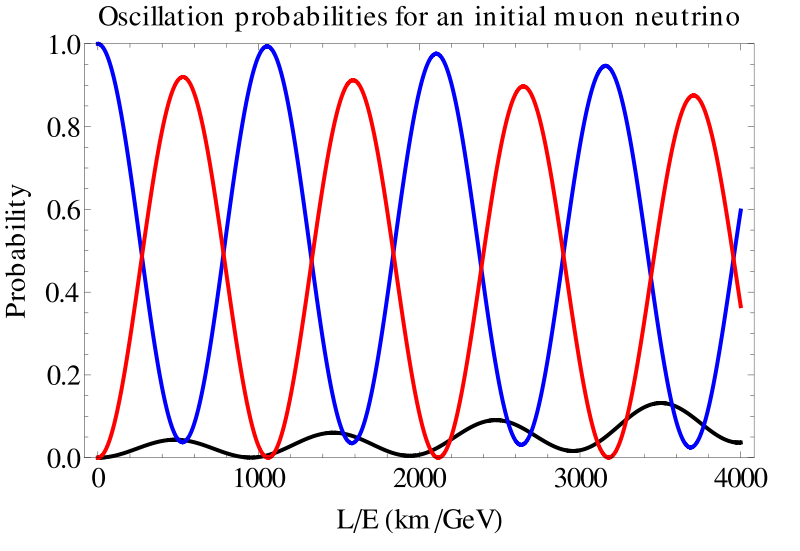
\includegraphics[width=1\textwidth]{figures/figures/osc_prob.png}
  \column{0.05\textwidth}
  \vspace{-70pt}

  \begin{equation*}
  \color{blue}
  \nu_\mu
  \end{equation*}
  \vspace{-20pt}
  \begin{equation*}
  \color{red}
  \nu_\tau
  \end{equation*}
  \vspace{-17pt}
  \begin{equation*}
  \nu_e
  \end{equation*}
  \gap
  \column{0.17\textwidth}
  ~

  \end{columns}


\end{center}


}


\frame
{
  \frametitle{Neutrino Oscillation in Vacuum}
  \begin{itemize}
  \bang Neutrinos are neutral leptons that interact weakly, they are produced in one of the flavor states
  \gap
  \bang Each flavor state, $l=e,\mu,\tau$,  is a superposition of three mass states, $\nu_1$, $\nu_2$, $\nu_3$
  \gap
  \begin{equation*}
|\nu_l \rangle = \sum_{\alpha = 1,}^3 U_{l\alpha}|\nu_\alpha \rangle
  \end{equation*}
  \gap
  \bang $U_{l\alpha}$ is an element in the Pontecorvo-Maki-Nakagawa-Sakata (PMNS) matrix
  \end{itemize}

}


\frame
{
  \frametitle{PMNS Matrix}
  \begin{itemize}
  \bang $U_{l\alpha}$ is an element in the Pontecorvo-Maki-Nakagawa-Sakata (PMNS) matrix
  \end{itemize}
  \begin{equation*}
 U = \begin{pmatrix} \label{pmns}
c_{13}c_{12}              &    c_{13}s_{12} 	   	 & 		s_{13} e^{-i\delta} \\
-s_{12}c_{23} - c_{12}s_{23}s_{13}e^{i\delta}	& c_{12}c_{23} - s_{12}s_{23}s_{13}e^{i\delta} 				& 		c_{13}s_{23}  \\
s_{23}s_{12} - c_{12}c_{23}s_{13}e^{i\delta}	& -c_{12}s_{23} - s_{12}c_{23}s_{13}e^{i\delta} 				& 		c_{13}c_{23}  \\
\end{pmatrix}
\end{equation*}
\begin{center}
\footnotesize
$c_{ij} = \cos(\theta_{ij})$

$s_{ij} = \sin(\theta_{ij})$
\end{center}
 \gap
  \begin{itemize}
\bang Unitary matrix representing a rotation in a complex 3 dimensional space
\gap
\bang Three Euler angles, $\theta_{12}$, $\theta_{23}$, $\theta_{13}$
\gap
\bang Complex phase $\delta$: potential for CP violation
  \end{itemize}
}

\frame
{
  \frametitle{Neutrino Oscillation in Vacuum}
  \begin{itemize}
	\bang Oscillation is a result of time evolution:
	\begin{equation*}
		|\nu_l(t) \rangle = \sum_{\alpha = 1,}^3 U_{l\alpha}e^{-iE_\alpha t}|\nu_\alpha \rangle
	\end{equation*}
	\bang For relativistic neutrinos, we approximate the energy and take $t \rightarrow L$, which we substitute into the time evolution:
	\begin{equation*}
		|\nu_l(L) \rangle = e^{-iEL} \sum_{\alpha = 1,}^3 U_{l\alpha}e^{-i\frac{m_\alpha^2}{2E} L}|\nu_\alpha \rangle
	\end{equation*}
  \gap
	\bang The factor $e^{-i\frac{m_\alpha^2}{2E} L}$ gives rise to oscillation


  \end{itemize}
}

\frame
{
  \frametitle{Neutrino Oscillation in Vacuum}
  \begin{itemize}
  \bang From the last slide
	\begin{equation*}
		|\nu_l(L) \rangle = e^{-iEL} \sum_{\alpha = 1,}^3 U_{l\alpha}e^{-i\frac{m_\alpha^2}{2E} L}|\nu_\alpha \rangle
	\end{equation*}
\bang Oscillation probability is the inner product
  \begin{equation*}
P_{l\rightarrow m} = 	 |\langle \nu_m|\nu_l \rangle|^2
	\end{equation*}
	\bang We then find the oscillation probability:
	\begin{equation*}\begin{split}
P_{l\rightarrow m}(L) =  \delta_{lm} - 4  \sum_{\alpha > \beta}  \Re(U^*_{l\alpha}U_{m\alpha}U^*_{l\beta}U_{m\beta}) \sin^2 \bigg(\frac{\Delta m_{\alpha\beta}^2}{4E} L\bigg) \\
 + 2  \sum_{\alpha>\beta}  \Im(U^*_{l\alpha}U_{m\alpha}U^*_{l\beta}U_{m\beta}) \sin\bigg(\frac{\Delta m_{\alpha\beta}^2}{2E}L\bigg)
\end{split}\end{equation*}
	\bang Dynamic behavior is in sine terms, mixing angles enter through U


  \end{itemize}
}


\frame
{
  \frametitle{Current Oscillation Parameter Measurements}

  \begin{columns}[c]
    \column{0.57\textwidth}

      \begin{itemize}
   \bang Experiments have contrained mixing angles and mass differences
\bang Unknown whether $\theta_{23}$ is exactly $45^\circ$
\bang Mass ordering is unknown: sign of $\Delta m_{32}^2$
\bang The CP-violating phase $\delta$ is not well constrained (matter/antimatter)
\end{itemize}
  \column{0.45\textwidth}
  \footnotesize \centering
  \begin{tabular}{ c |  c }
Parameter & PDG Average \\  \hline
  $\sin^2\big(\theta_{12}\big)$&$  0.304 \pm0.014$  \\
  $\sin^2\big(\theta_{23}\big)$&$  0.514_{-0.056}^{+0.055}                  $   \\
  $\sin^2\big( \theta_{13}\big)$&$  0.0219 \pm0.0012$  \\
    $\Delta m^2_{21}       $&$ (7.53 \pm 0.18) \times 10^{-5}$ eV${}^2$ \\
  $|\Delta m^2_{32}|       $&$ (2.42 \pm 0.06 ) \times 10^{-3}$ eV${}^2$  \\
\end{tabular}

  \end{columns}
  \gap
  \gap
\begin{columns}[c]

  \column{0.45\textwidth}
  \centering
  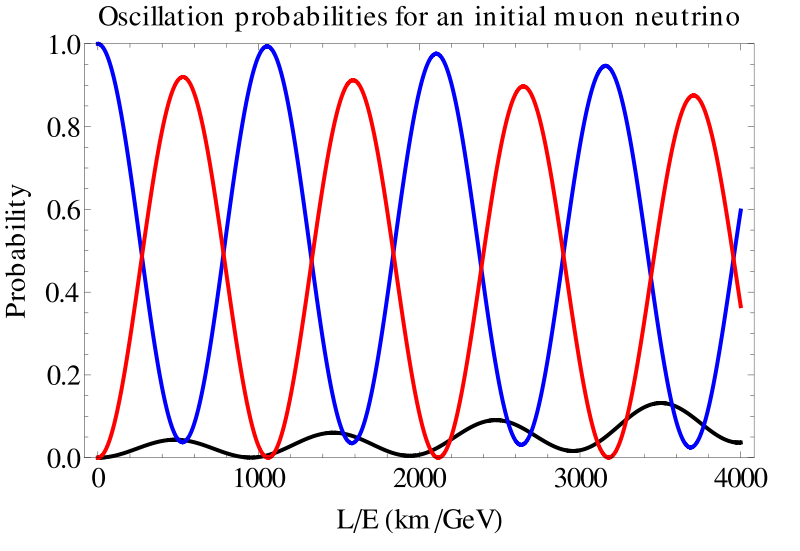
\includegraphics[width=1\textwidth]{figures/figures/osc_prob.png}
  \column{0.05\textwidth}
  \vspace{-50pt}

  \begin{equation*}
  \color{blue}
  \nu_\mu
  \end{equation*}
  \vspace{-20pt}
  \begin{equation*}
  \color{red}
  \nu_\tau
  \end{equation*}
  \vspace{-17pt}
  \begin{equation*}
  \nu_e
  \end{equation*}
  \gap
  \column{0.05\textwidth}
  ~

\column{0.4\textwidth}
\centering
 \begin{figure} 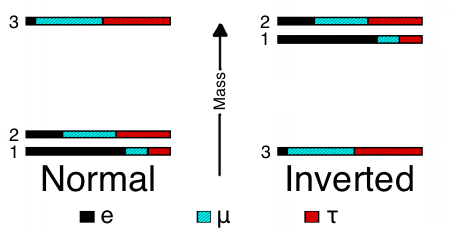
\includegraphics[width=\textwidth]{figures/figures/hierarchy.jpg} \end{figure}
 \vspace{8pt}
\end{columns}
}


\begin{frame}
\app{\nova (\textit{noun})}{An experiment which aims to answer remaining questions surrounding neutrino oscillation}
\end{frame}


\frame
{
\frametitle{\nova}

\begin{columns}[c]
\column{0.6\textwidth}

\begin{itemize}
\bang  \textbf{NuMI} is a neutrino source at Fermilab
\bong (Neutrinos at the Main Injector)
  \begin{itemize}
  \bing Mostly \numu
  \end{itemize}
\gap
\bang \textbf{\nova} is a neutrino oscillation experiment
\bong (NuMI Off-axis $\nu_e$ Appearance)
  \begin{itemize}
  \bing Two functionally identical detectors
  \bing 14 mrad off-axis
  \bing Narrow energy peak near 2 GeV

  \end{itemize}
\gap

\end{itemize}
\centering \footnotesize
\gap
\begin{tabular}{l | c | c}
& Near Detector & Far Detector  \\ \hline
Baseline (km)& 1  & 810   \\ \hline
Mass (kton) & 0.3 & 14  \\ \hline
Channels & 20,192 & 344,064  \\ %\hline
\end{tabular}

%{ \centering
%\includegraphics[width=1\textwidth]{figures/earth.png}}

\column{0.4\textwidth}
\centering
\vspace{-5pt}
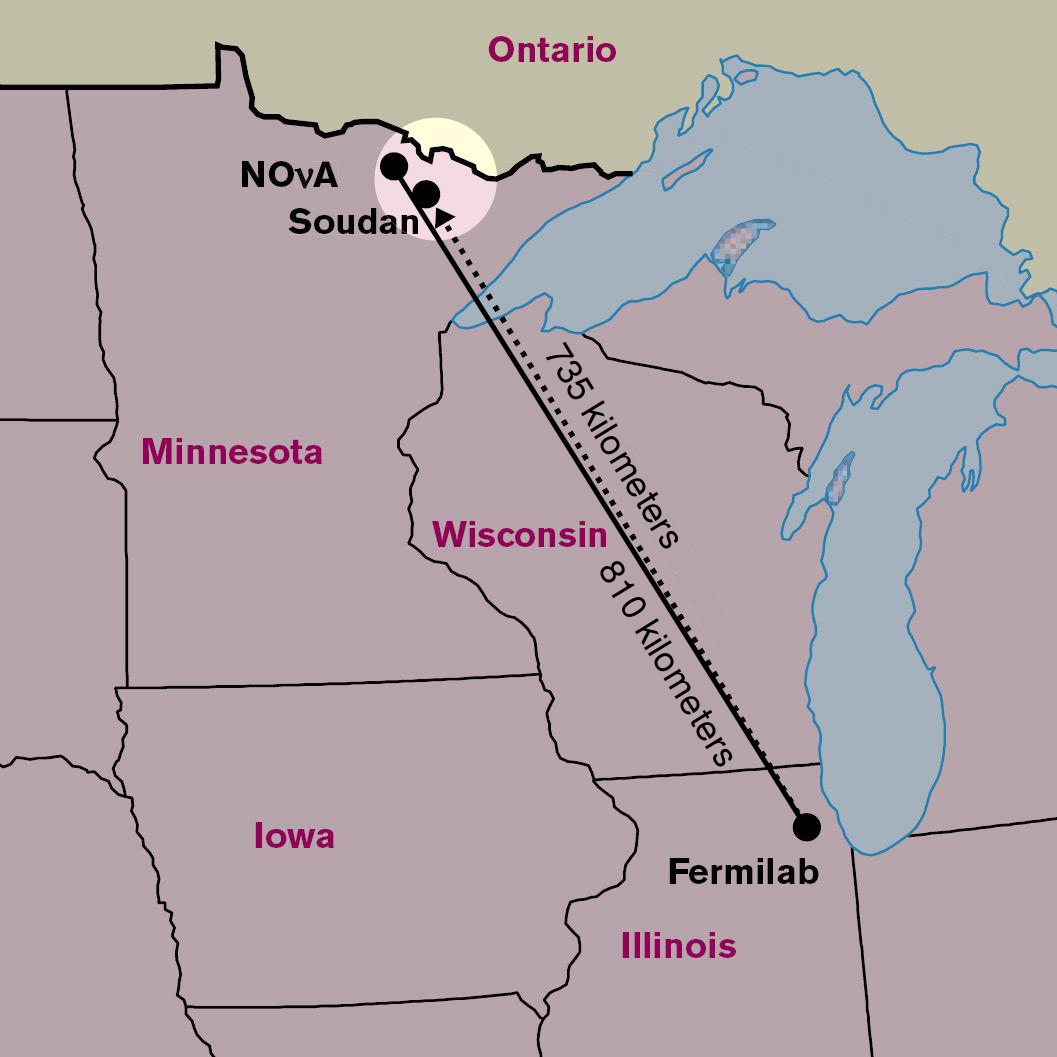
\includegraphics[width=1\textwidth]{figures/figures/map.png}

\vspace{7pt}

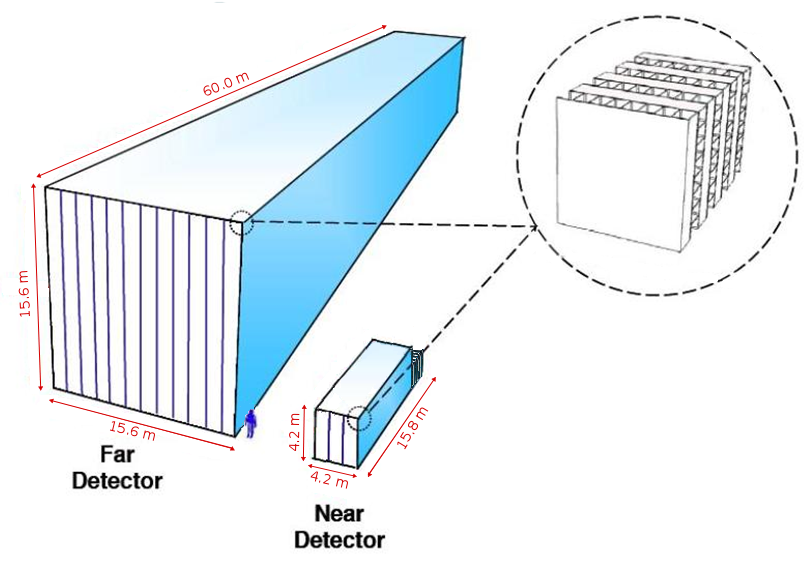
\includegraphics[width=1\textwidth]{figures/figures/detectors.png}

\end{columns}


}

\frame
{
  \frametitle{NuMI}
    \begin{itemize}
	\bang High energy protons from are directed into a graphite target
	\bang These collisions produce a shower of particles
	\bang Shower is primarily pions and kaons
	\bang Muons are absorbed in steel plates and rock to leave behind a beam of muon-neutrinos
	\begin{figure} 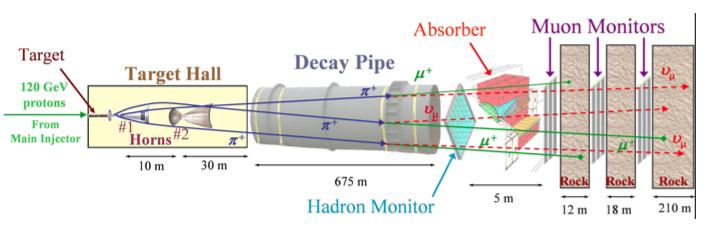
\includegraphics[width=0.85\textwidth]{figures/figures/numi.png} \end{figure}
\end{itemize}

}

\frame
{
\frametitle{\nova Detectors}

\begin{itemize}
\bang Basic unit of \nova detectors is an extruded PVC cell
\bang Cells are filled with liquid scintillator
\bang Wavelength-shifting fiber transmits scintillation light to readout
\bang Avalanche photo-diodes capture light output from fiber
\end{itemize}

\begin{columns}[c]
\column{0.08\textwidth}

\column{0.2\textwidth}
\centering
 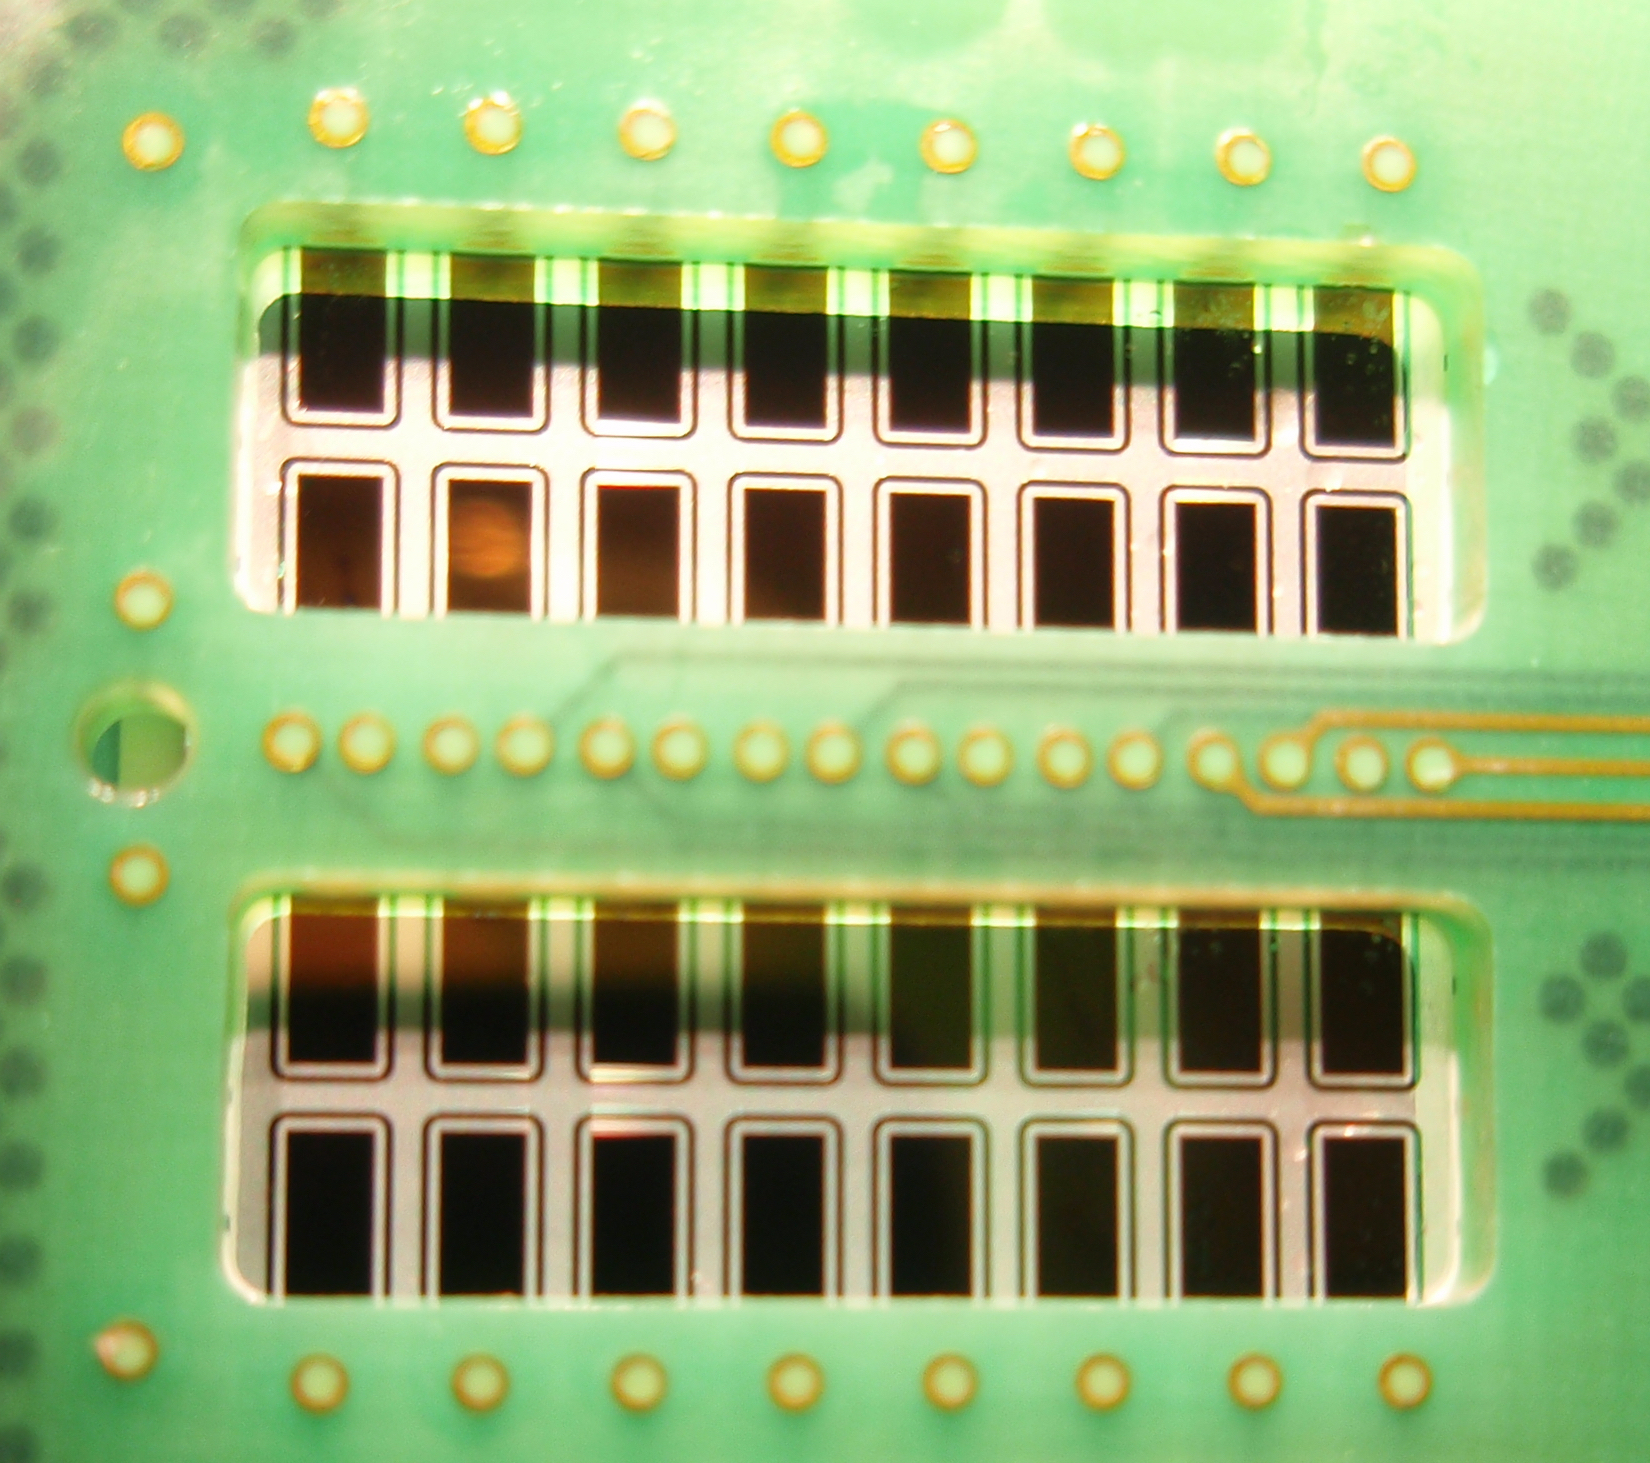
\includegraphics[width=0.8\textwidth]{figures/figures/apd_zoom.jpeg}

 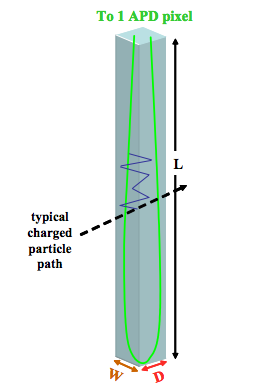
\includegraphics[width=1\textwidth]{figures/figures/cell.png}
\column{0.8\textwidth}

\centering
 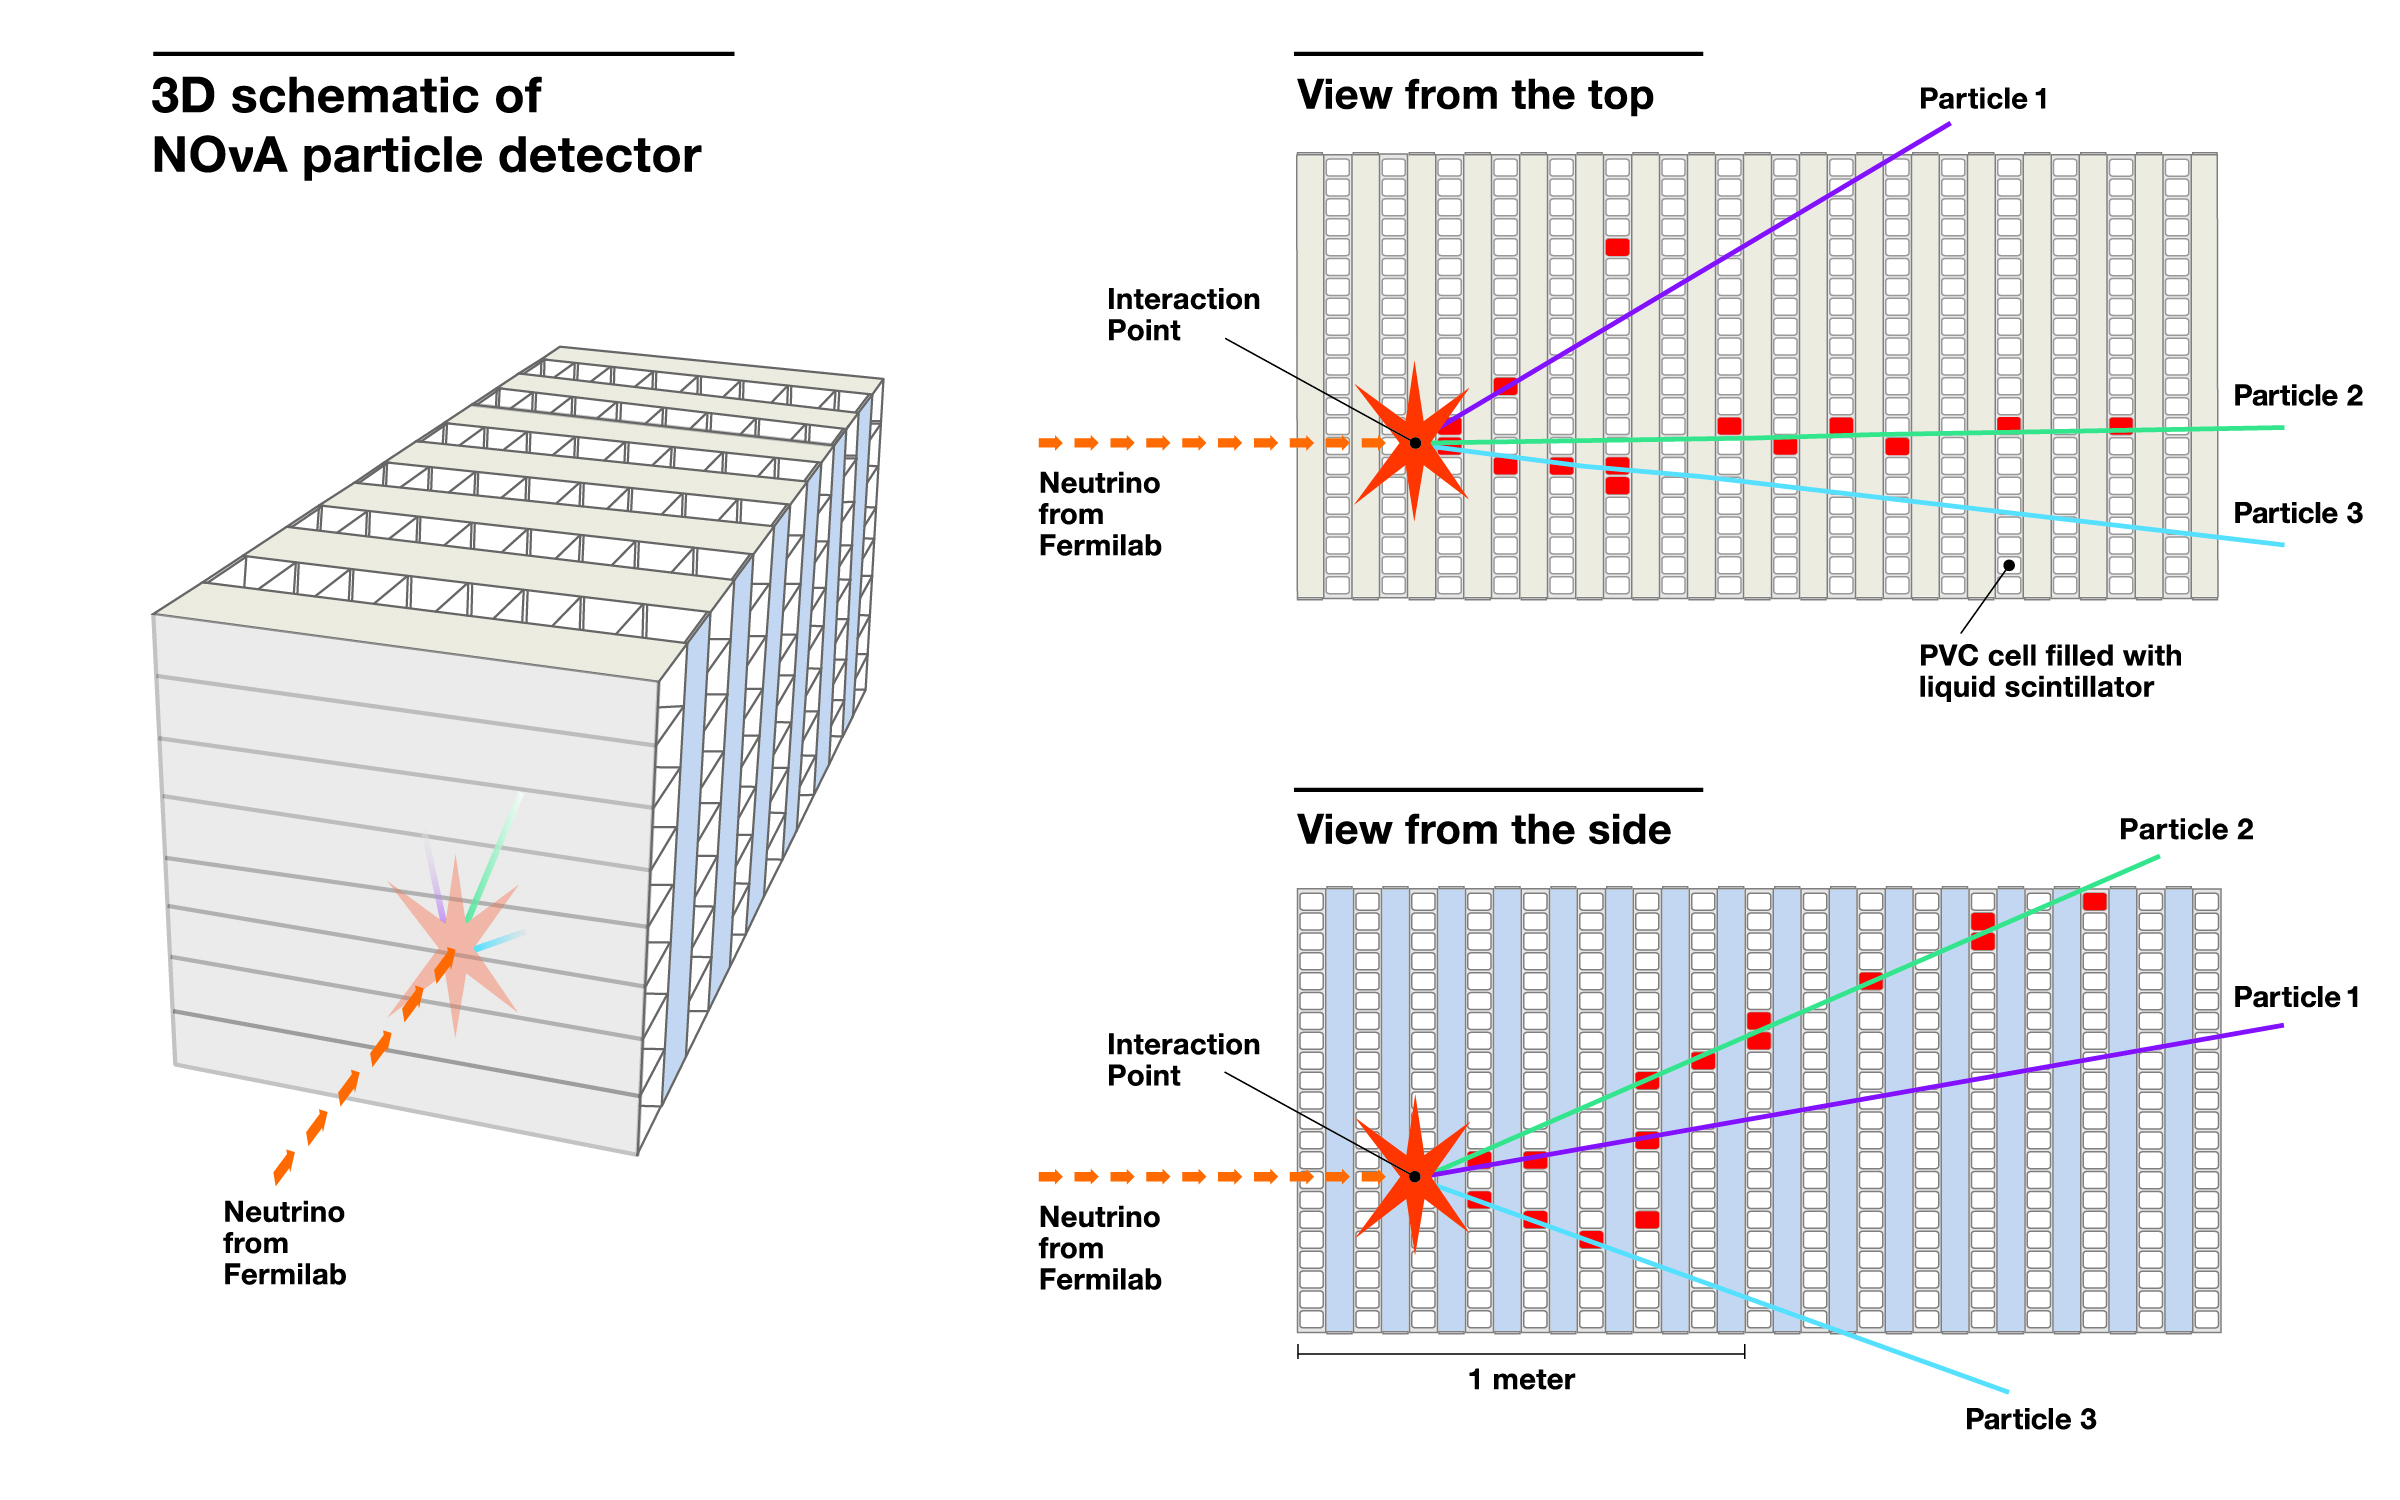
\includegraphics[width=0.85\textwidth]{figures/figures/schematic.jpg}

 {\scriptsize Illustration courtesy of Fermilab}

\end{columns}




}




\frame
{
  \frametitle{Far Detector}
  \centering
\begin{columns}[c]
\column{0.5\textwidth}
\centering
 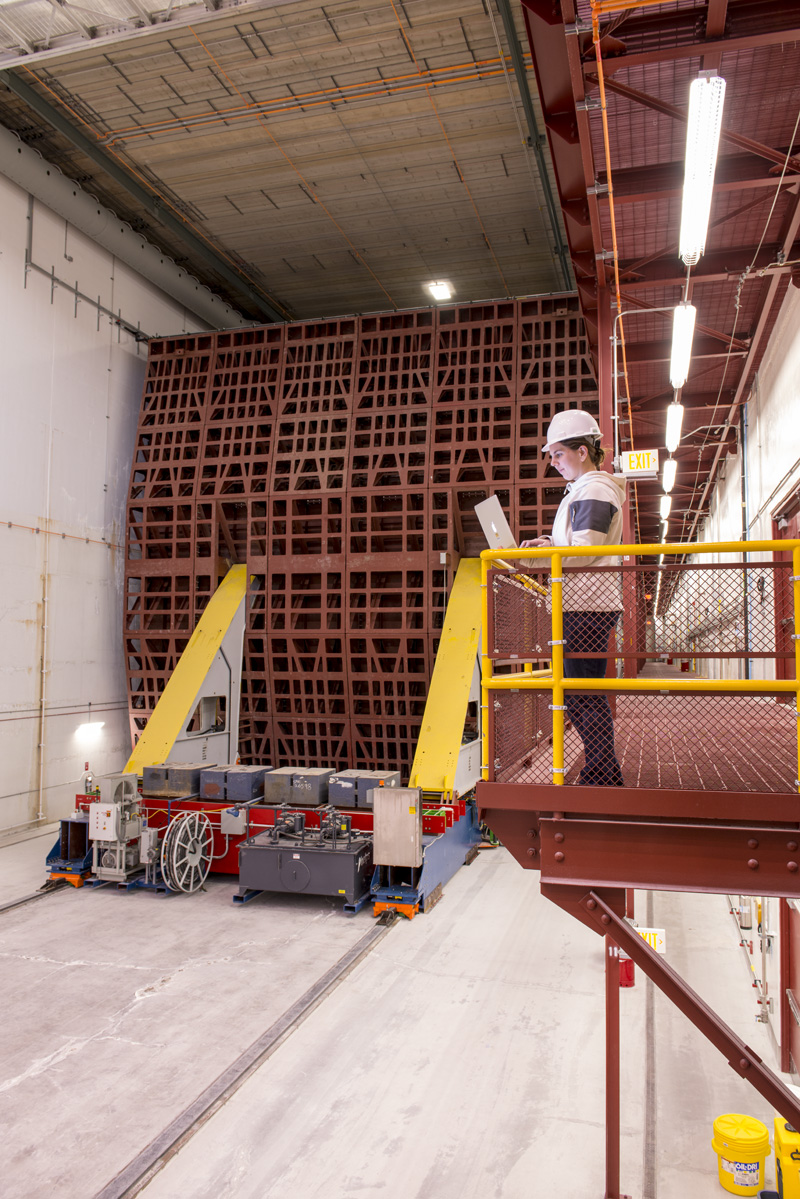
\includegraphics[height=0.85\textheight]{figures/det_photos/det_front.jpg}

\column{0.5\textwidth}
\centering
 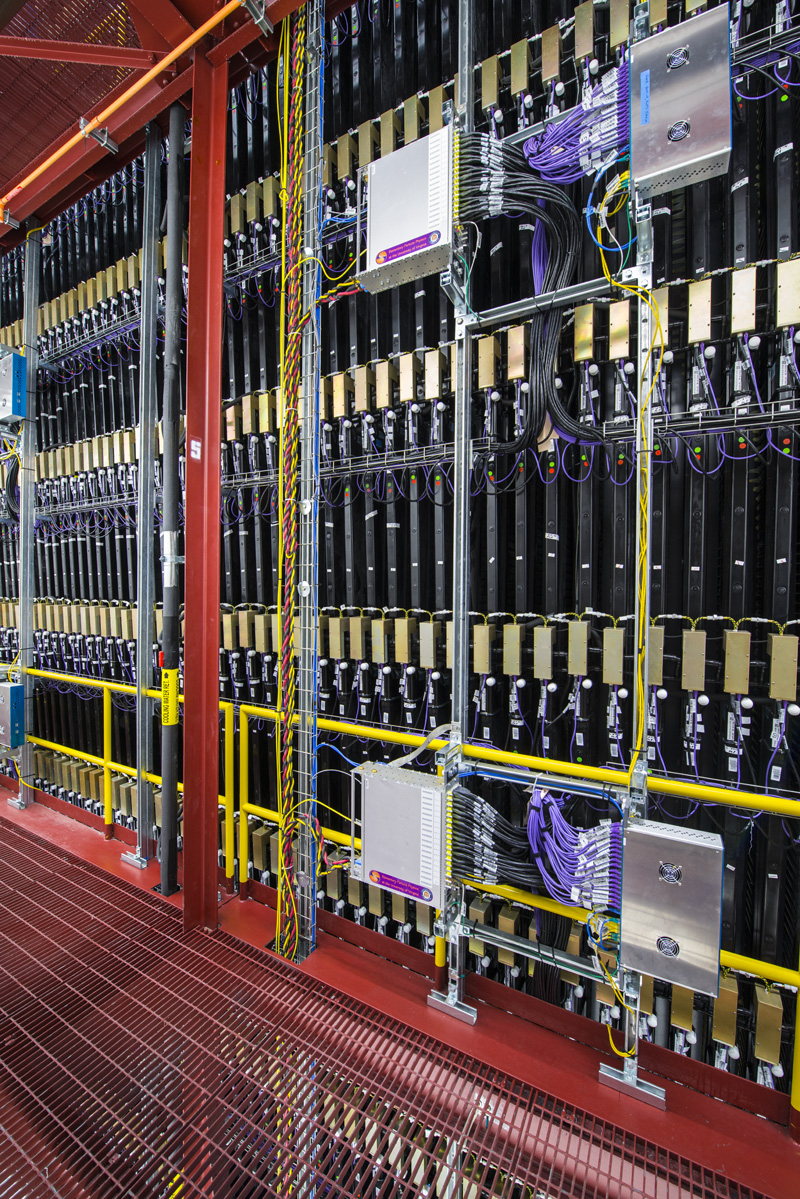
\includegraphics[height=0.85\textheight]{figures/det_photos/det_side.jpg}
\end{columns}
\gap
{\scriptsize Photos courtesy of Fermilab}


}

\frame
{
  \frametitle{Near Detector}
    \begin{itemize}
	\bang The Near Detector is considerably smaller
	\bang Installed in a 300 foot deep cavern at Fermilab

\end{itemize}
	\begin{figure} \includegraphics[height=0.55\textwidth]{figures/det_photos/ND.jpg} \end{figure}
}


\frame
{
  \frametitle{Near Detector}
	\begin{figure} 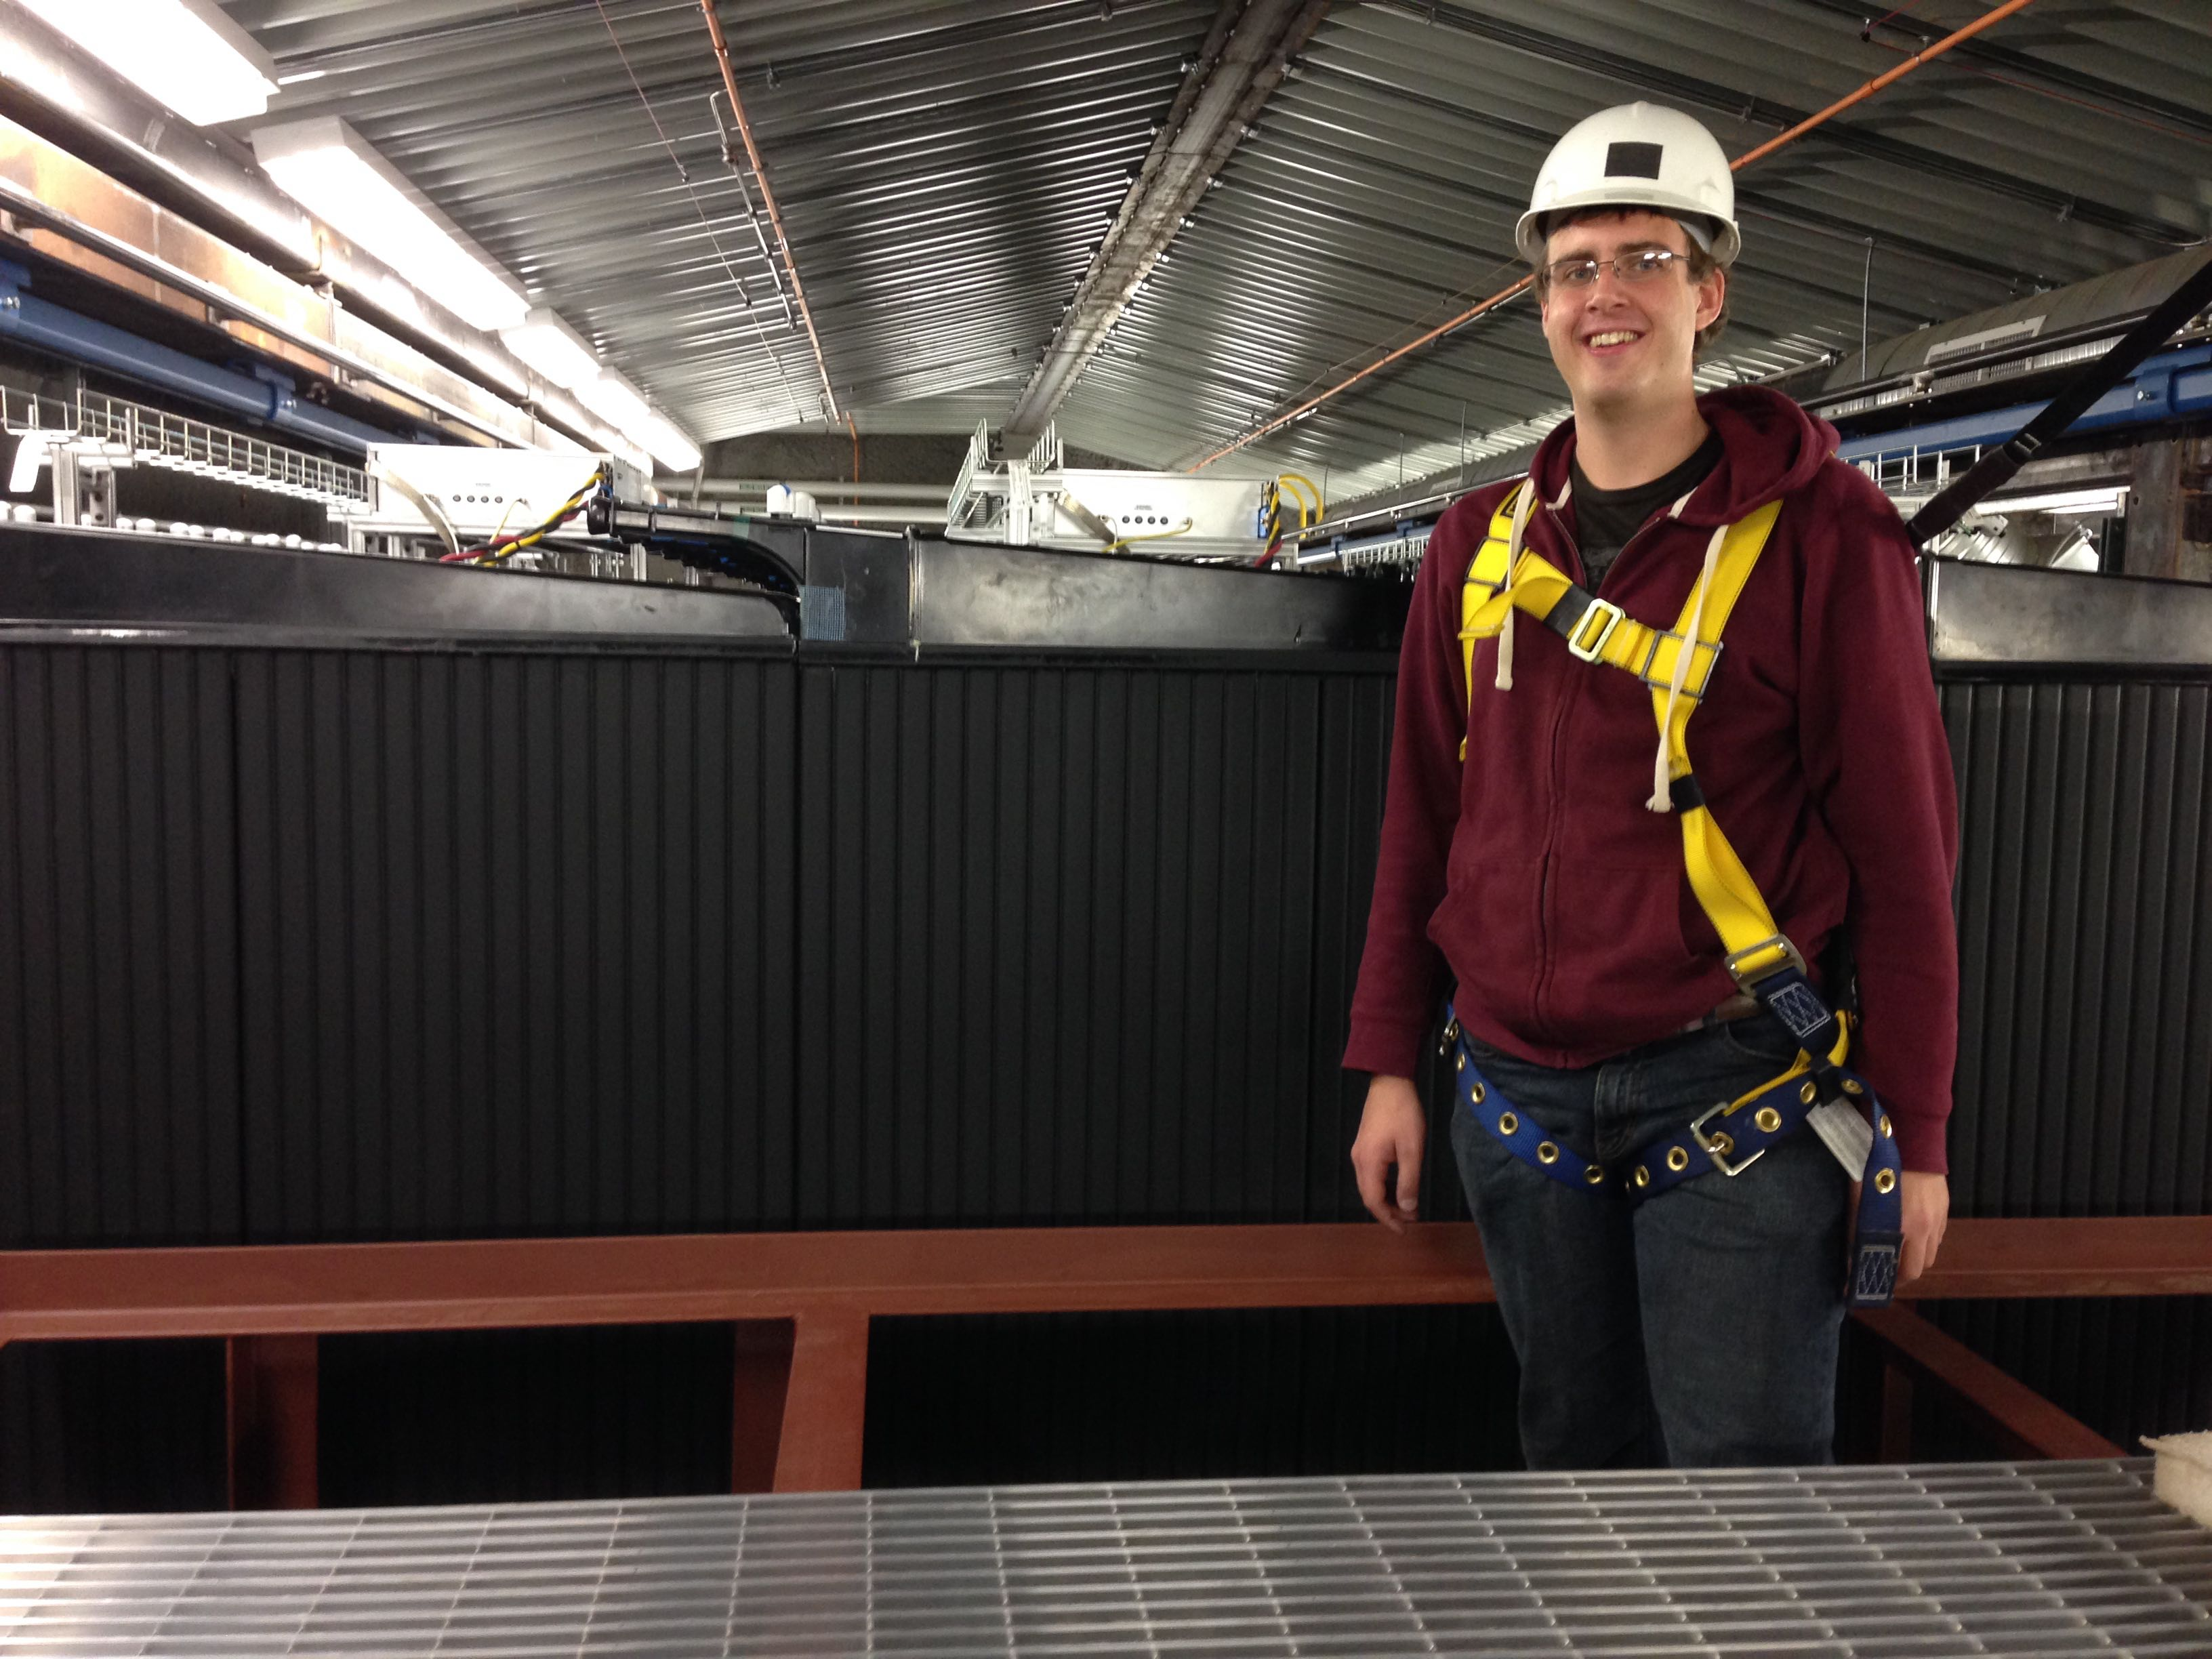
\includegraphics[height=0.55\textwidth]{figures/det_photos/meND_small.jpg} \end{figure}
}

\frame
{
  \frametitle{Event Topologies}

 \begin{figure} 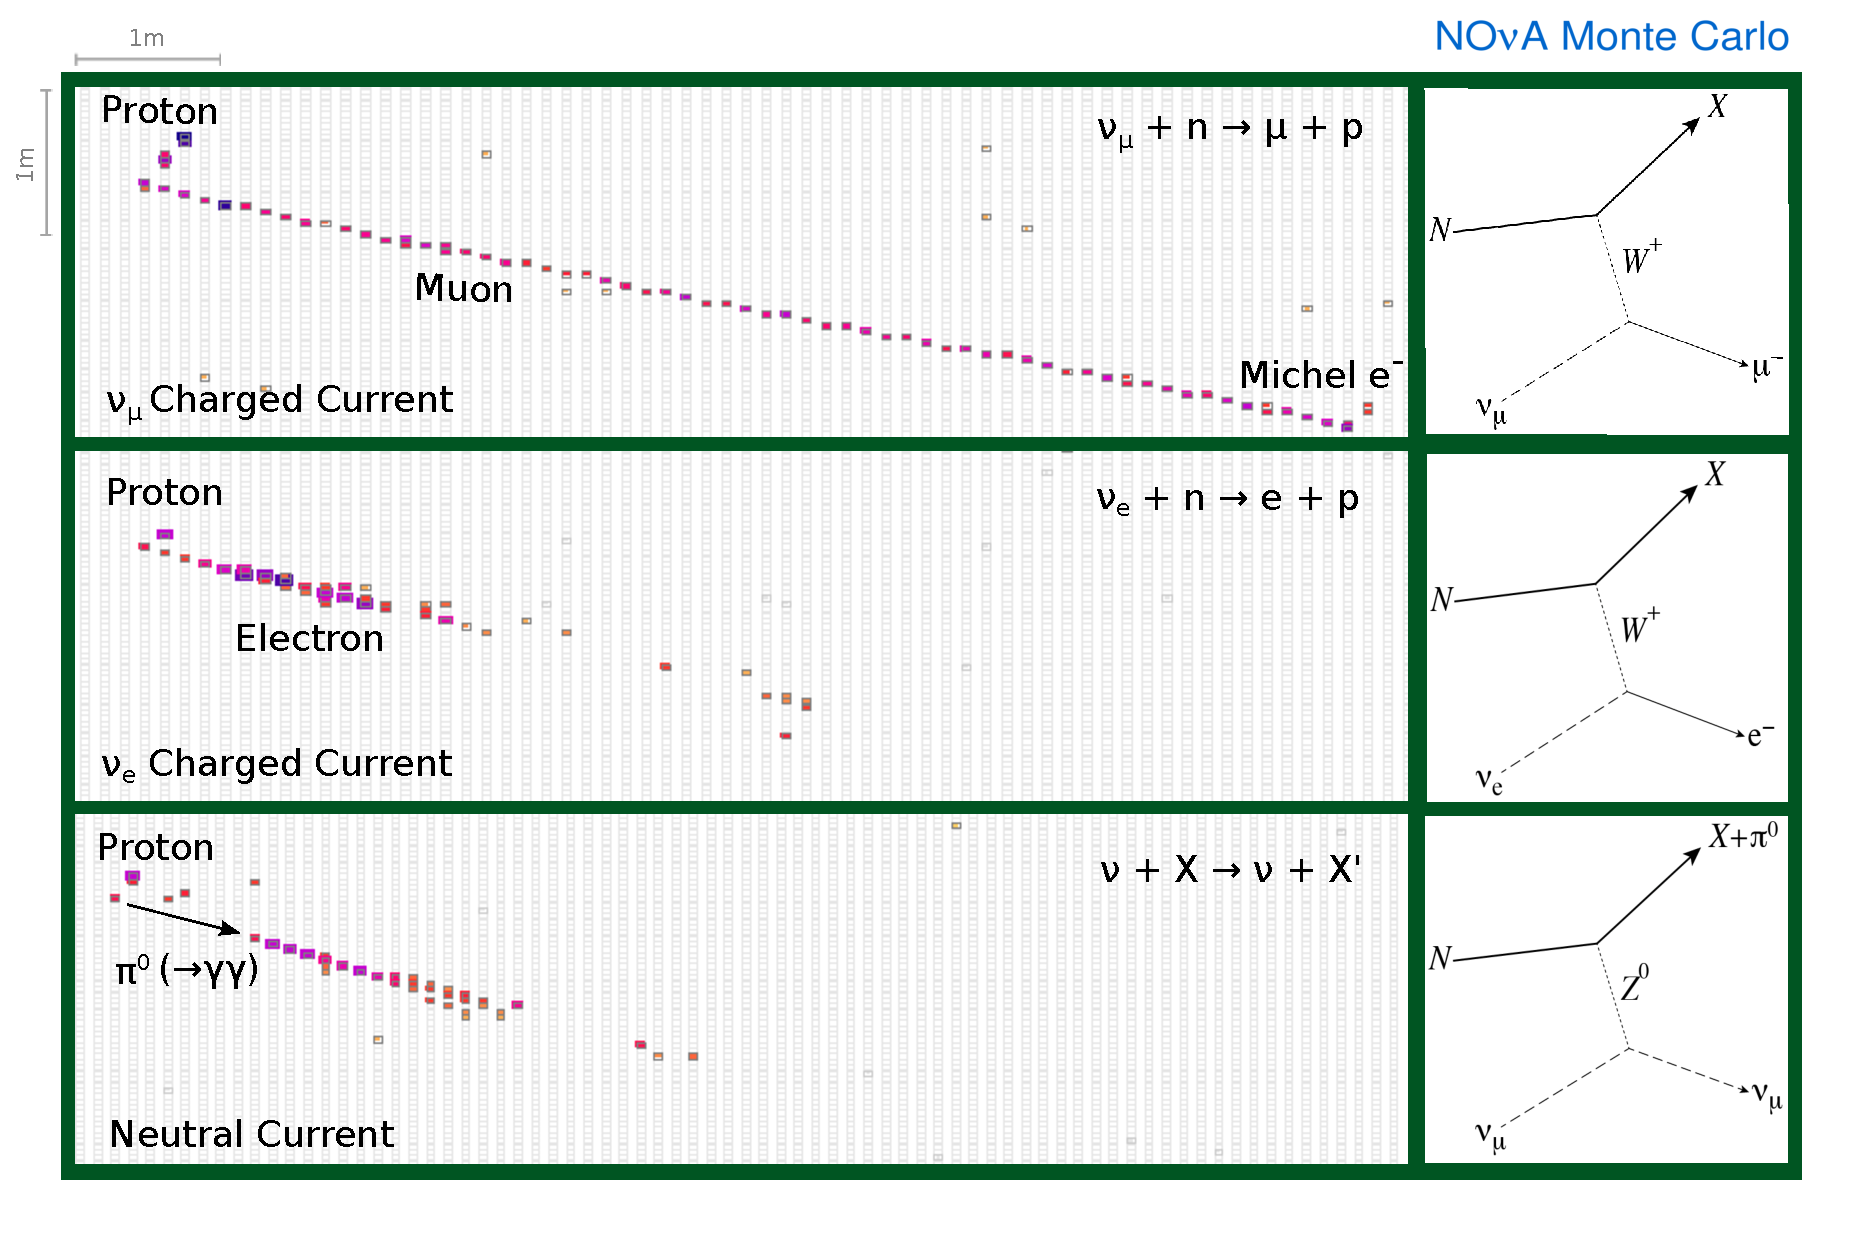
\includegraphics[width=0.9\textwidth]{figures/figures/event_topology_nue.pdf} \end{figure}
  \vspace{-15pt}
 \begin{center}
 \footnotesize Electromagnetic radiation length is $\sim$38 cm, \\
 spans several cells (4 cm $\times$ 6 cm)
 \end{center}

}

\frame
{
  \frametitle{Event Topologies}
\begin{columns}[]
\column{0.45\textwidth}
\begin{itemize}
\item Analysis signal: \numu charged-current events
\gap
\item Muon present
\gap
\item Hadron shower topology varies
\end{itemize}
\column{0.55\textwidth}
 \begin{figure} 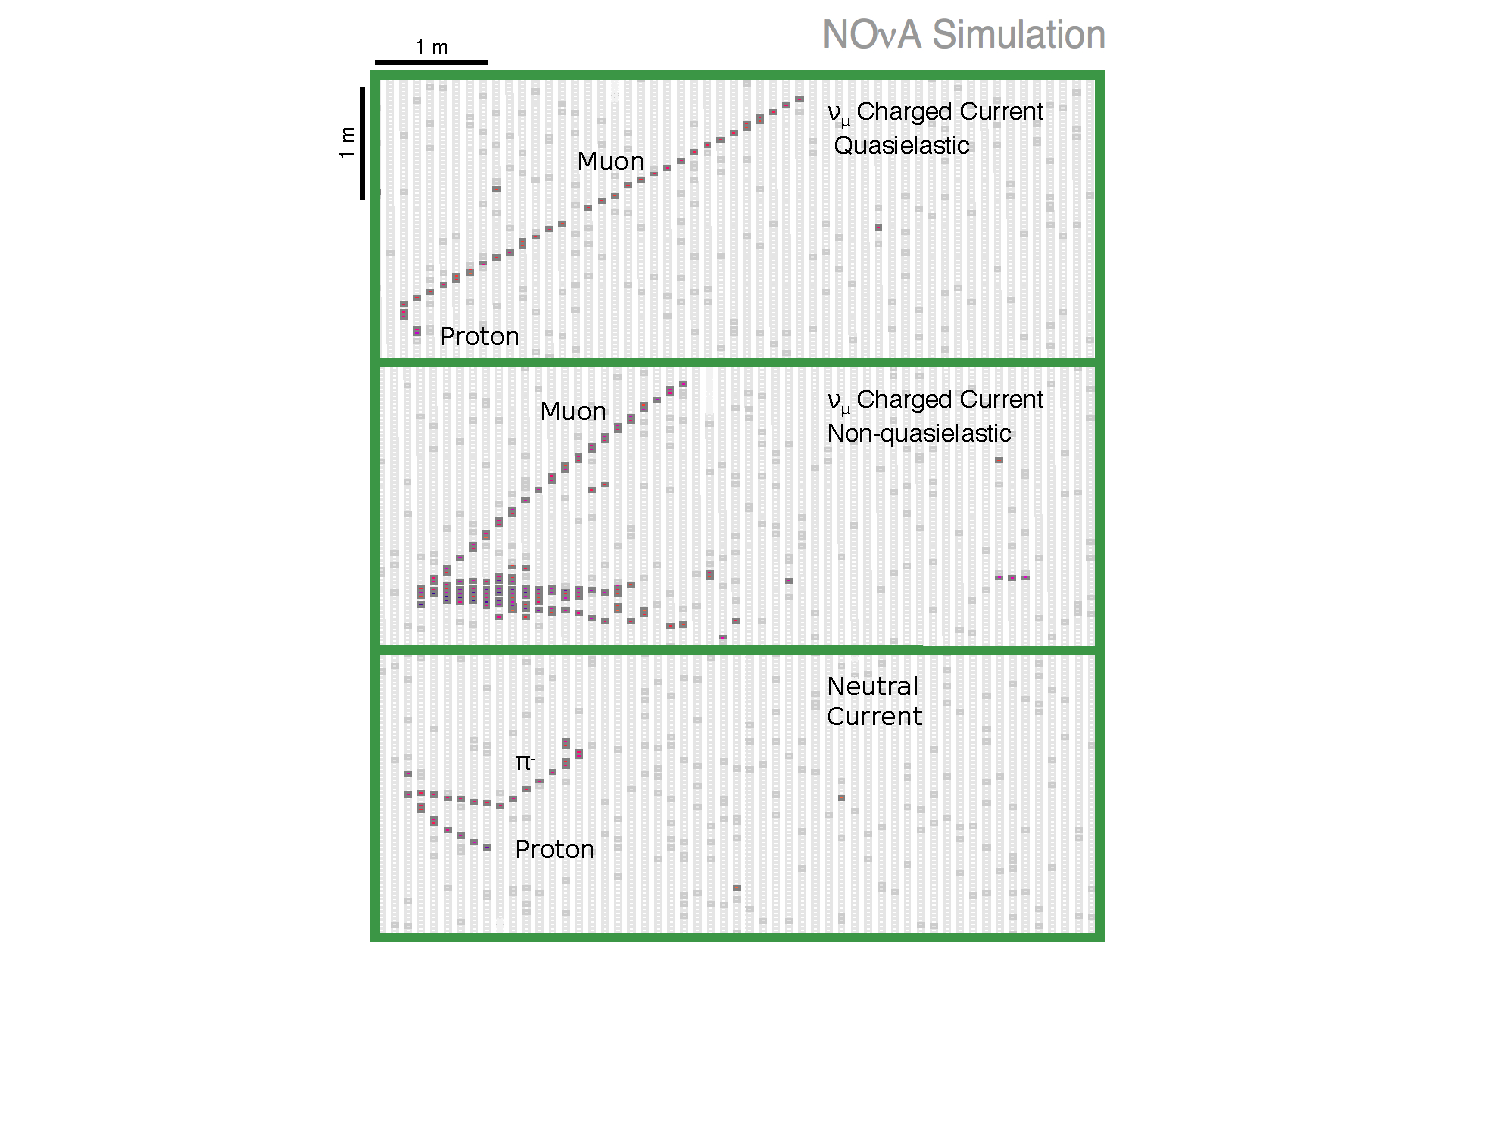
\includegraphics[width=\textwidth]{figures/figures/event_topology_numu.pdf} \end{figure}

\end{columns}

}


\frame
{
  \frametitle{Real Far Detector Data}

 \begin{figure} 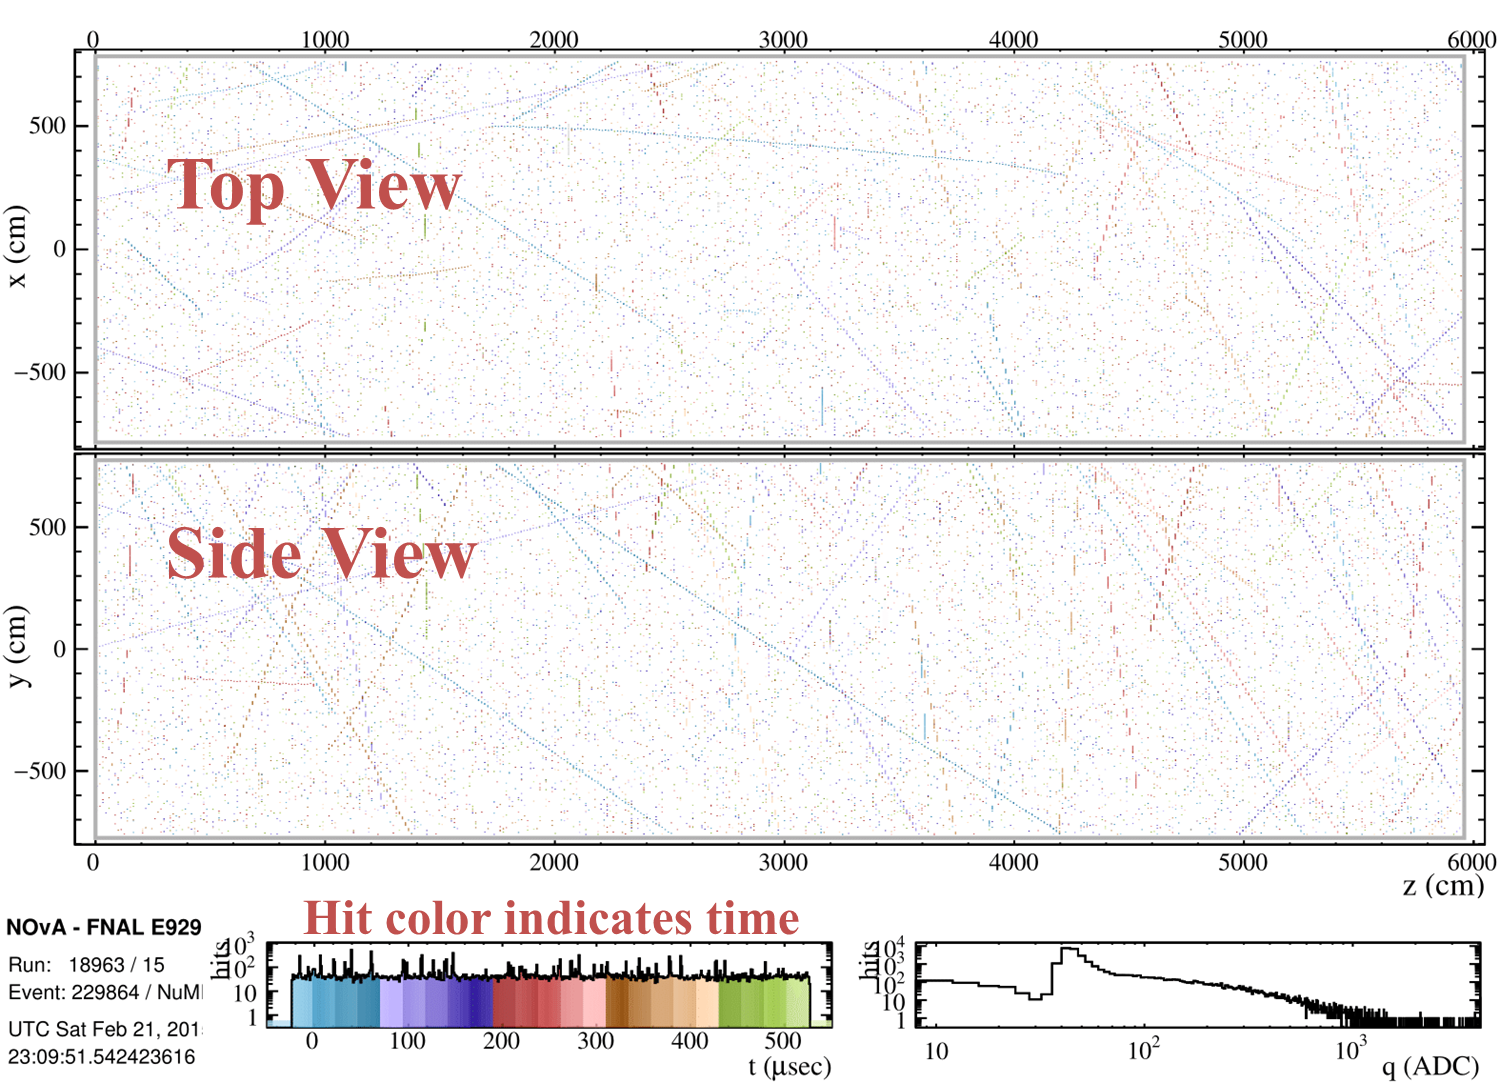
\includegraphics[width=0.85\textwidth]{figures/evd_steps/evd_top_side.png} \end{figure}
 \centering \footnotesize $~$

}

\frame
{
  \frametitle{Real Far Detector Data}

 \begin{figure} 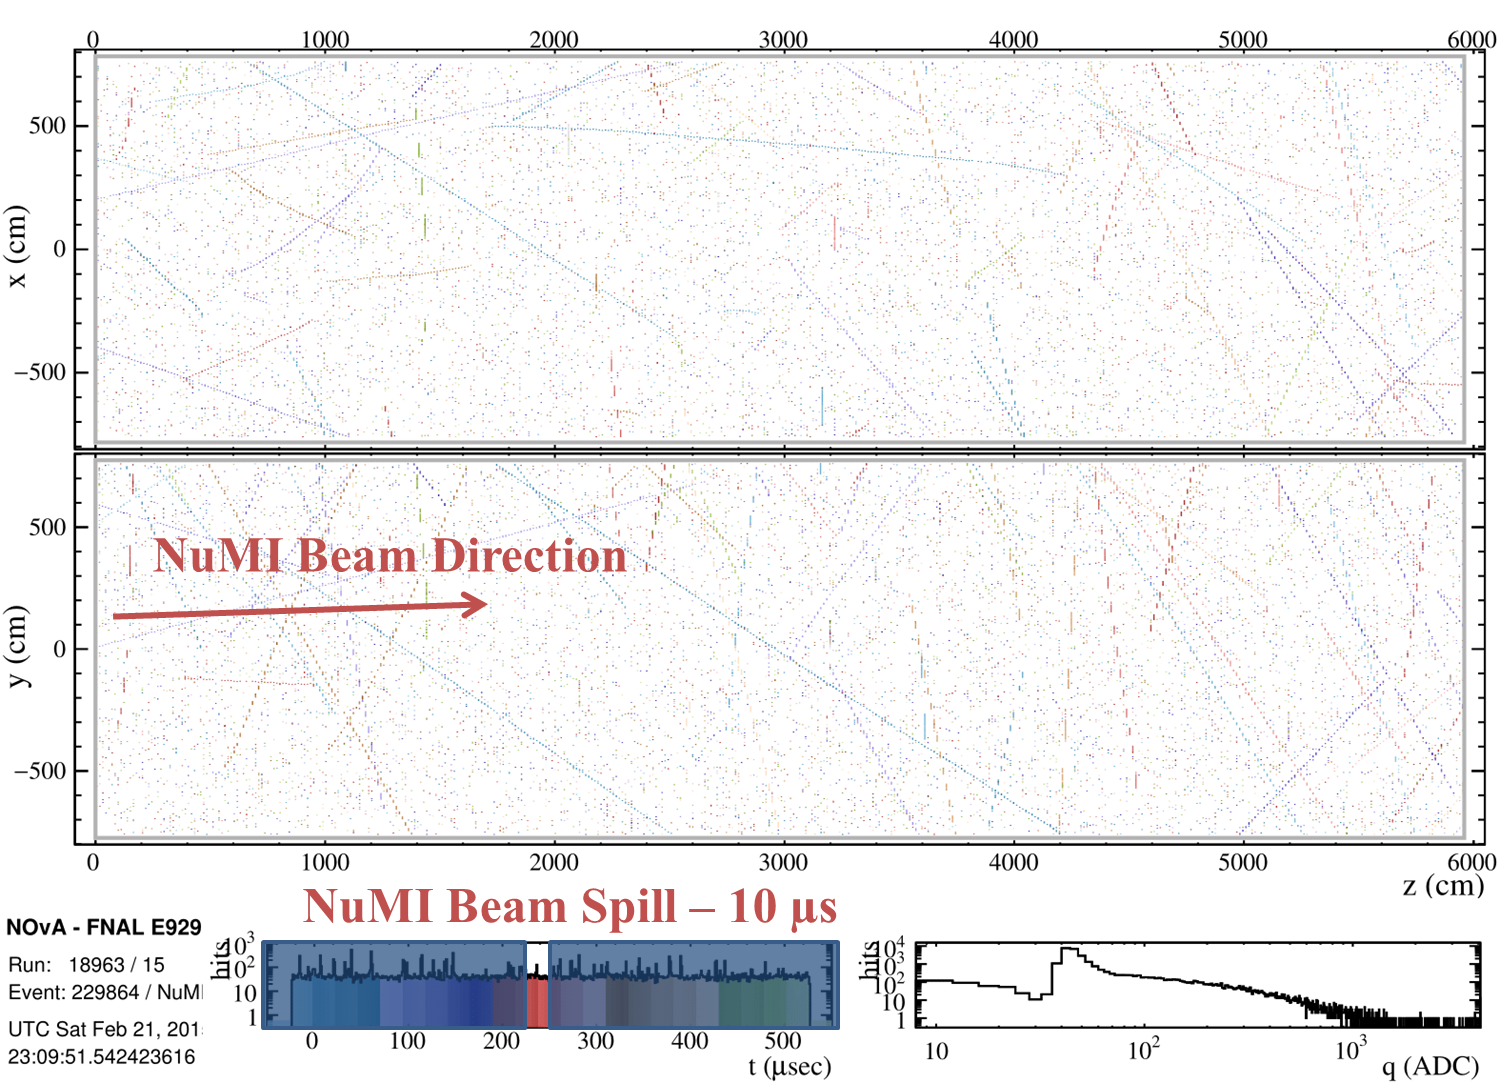
\includegraphics[width=0.85\textwidth]{figures/evd_steps/evd_beam_dir.png} \end{figure}
 \centering \footnotesize Analysis uses over 10 million beam spills, $\sim 2$ min exposure,  100 kHz cosmic ray rate
}

\frame
{
  \frametitle{Real Far Detector Data}

 \begin{figure} 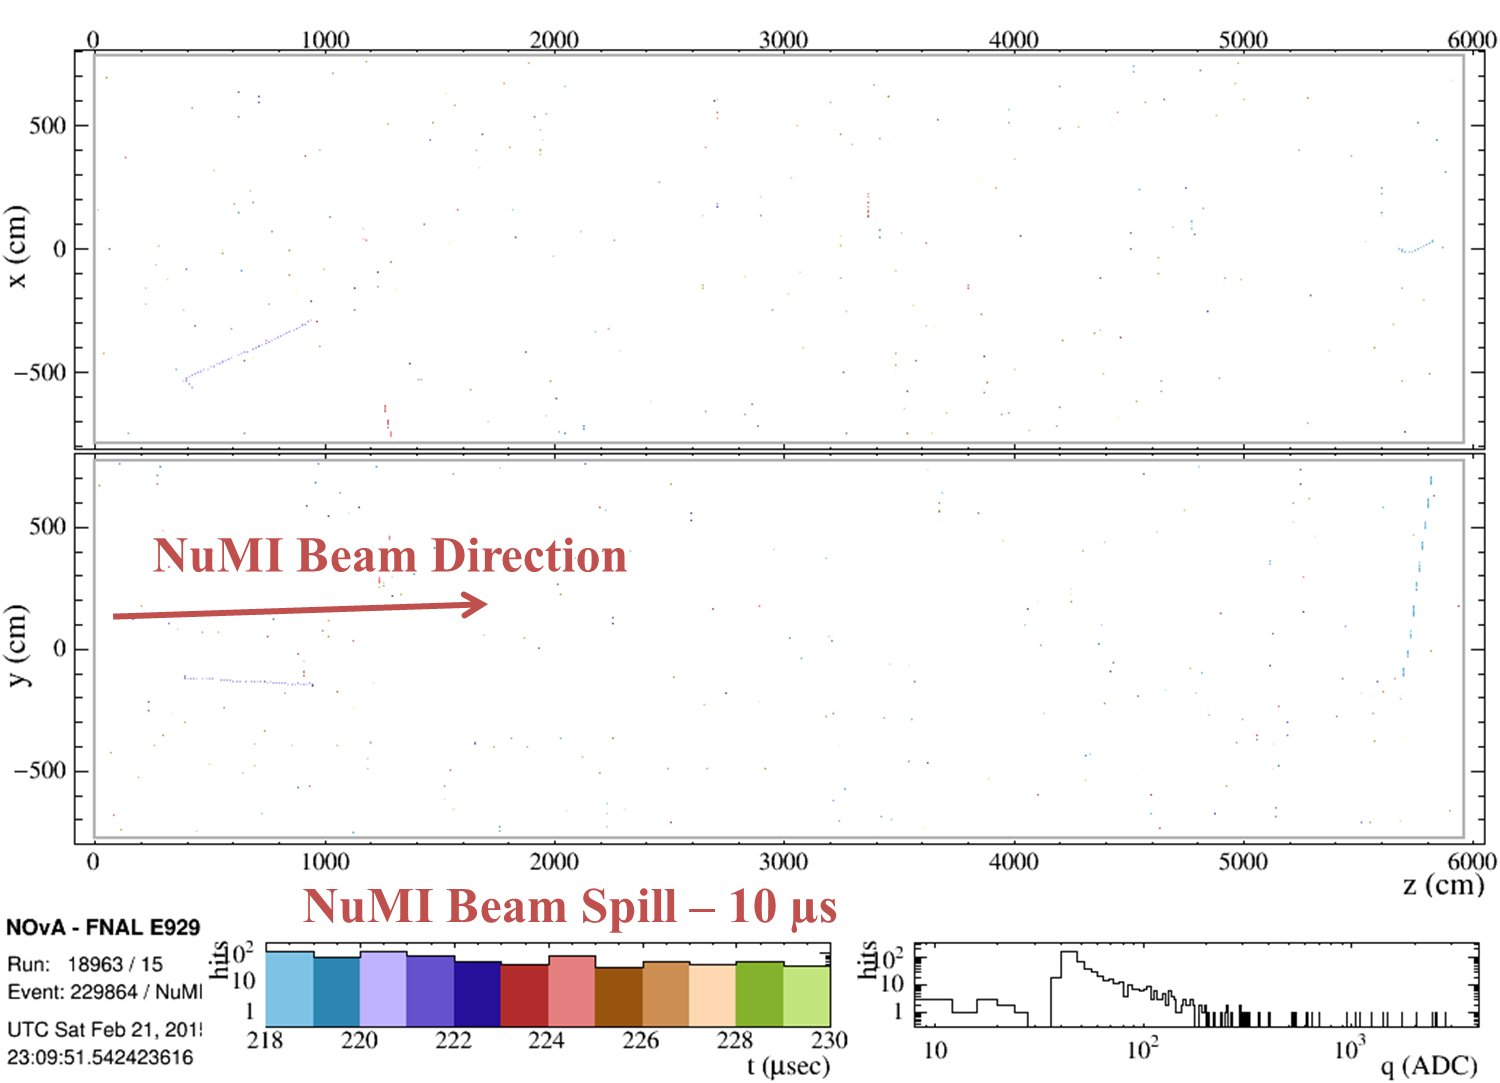
\includegraphics[width=0.85\textwidth]{figures/evd_steps/evd_beam_dir_nu.png} \end{figure}

 \centering \footnotesize $~$

}

\frame
{
  \frametitle{Real Far Detector Data}

 \begin{figure} 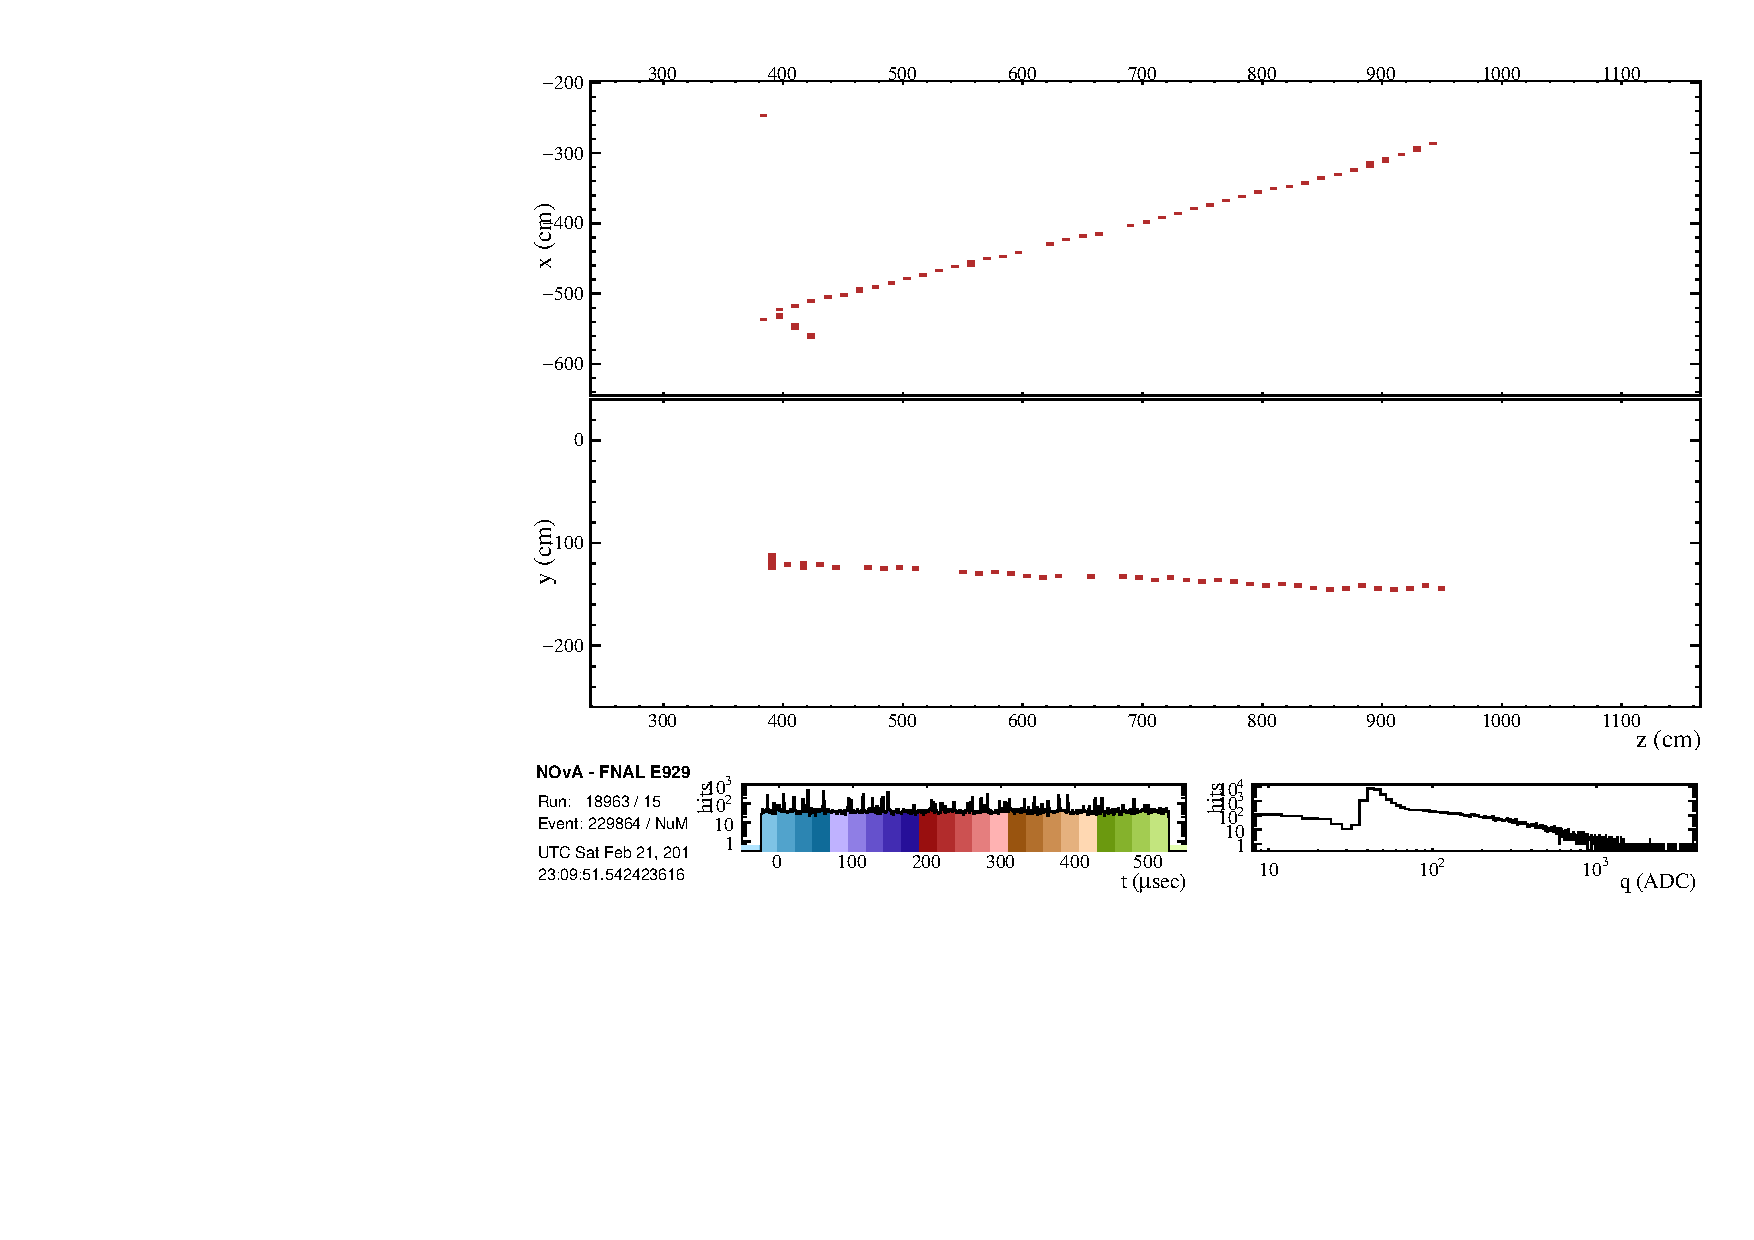
\includegraphics[height=0.85\textwidth, angle=-90]{figures/evd_steps/evd_oneslicehit.pdf} \end{figure}
  \centering \footnotesize $~$


}


\frame{
\frametitle{Oscillation Analysis}
\begin{tikzpicture}[]
   % Place nodes
   \node [block] (reco) {Reconstruction};
    \node [block, right = 2.7cm, right of=reco] (energy) {Energy Estimation};
   \node [block, right = 2.7cm, right of=energy, fill=emerald] (sel) {Event Selection};
    \node [block, below = 1.0cm, below of=sel] (nd) {Near Detector Data};
    \node [block, below = 2.5cm, below of=nd] (fd) {Far Detector Data};
   \node [block, left = 2.7cm, left of=nd] (eff) {Extrapolation};
   \node [block, left = 2.7cm, left of=eff] (extrap) {Prediction \\ \footnotesize{Function of oscillation parameters}};
%   \node [cloud, below =-0.5cm, below of=extrap] (fit) {Likelihood Fit};
\node[inner sep=0cm, below =2.5cm, below of=extrap, align=left] (fit)
    { 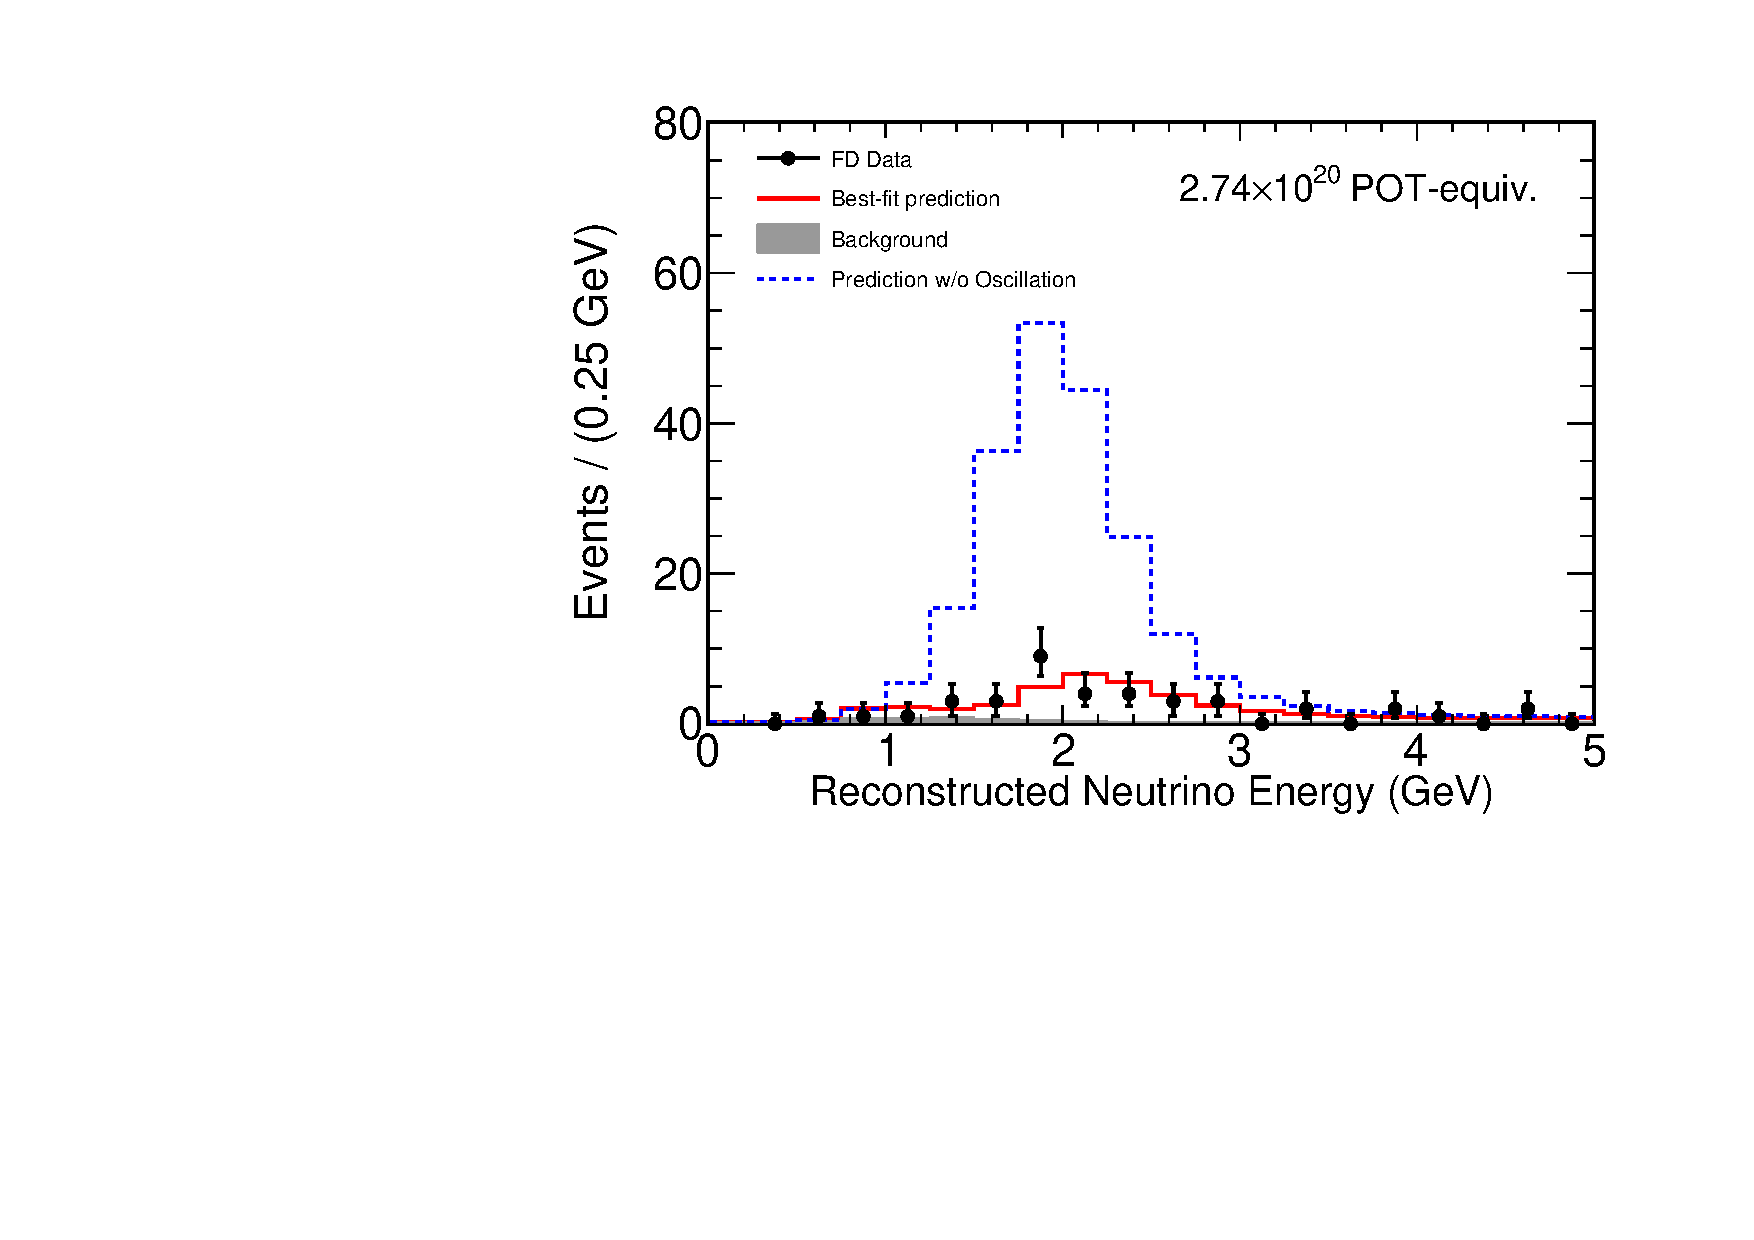
\includegraphics[width=.4\textheight, angle=-90]{figures/results/fd_data_mc_numi_plots/ccE_unblind_wUnosc.pdf}};
    \node [dot, right = 1.0cm, right of=sel] (bre){};
    \node [dot, right = 1.0cm, right of=fd] (brf){};
     \node [dot, right = 1.0cm, right of=nd] (brn){};

   % Draw edges
   \path [line] (reco) |- (energy);
    \path [line] (energy) |- (sel);
    \path [lin] (sel) -- (bre);
    \path [lin] (bre) -- (brf);
    \path [line] (brf) |- (fd);
    \path [line] (brn) |- (nd);
    \path [line] (nd) -- (eff);
    \path [line] (eff) -- (extrap);
    \path [line] (extrap) -- (fit);
    \path [line] (fd) -- (fit);


\end{tikzpicture}

}


\begin{frame}
\app{Reconstruction (\textit{noun})}{Extraction of patterns in raw data to aid in physics measurements}
\end{frame}


\begin{frame}

\frametitle{Reconstruction}
\framesubtitle{Slicing}

\begin{itemize}
\item First step is to resolve individual particle interactions
\gap
\item Activity is clustered in time and space to form \textit{slices}
\end{itemize}
\gap
\gap
\begin{columns}[b]
\column{0.5\textwidth}
\centering
\textcolor{custom_red}{Before Slicing}
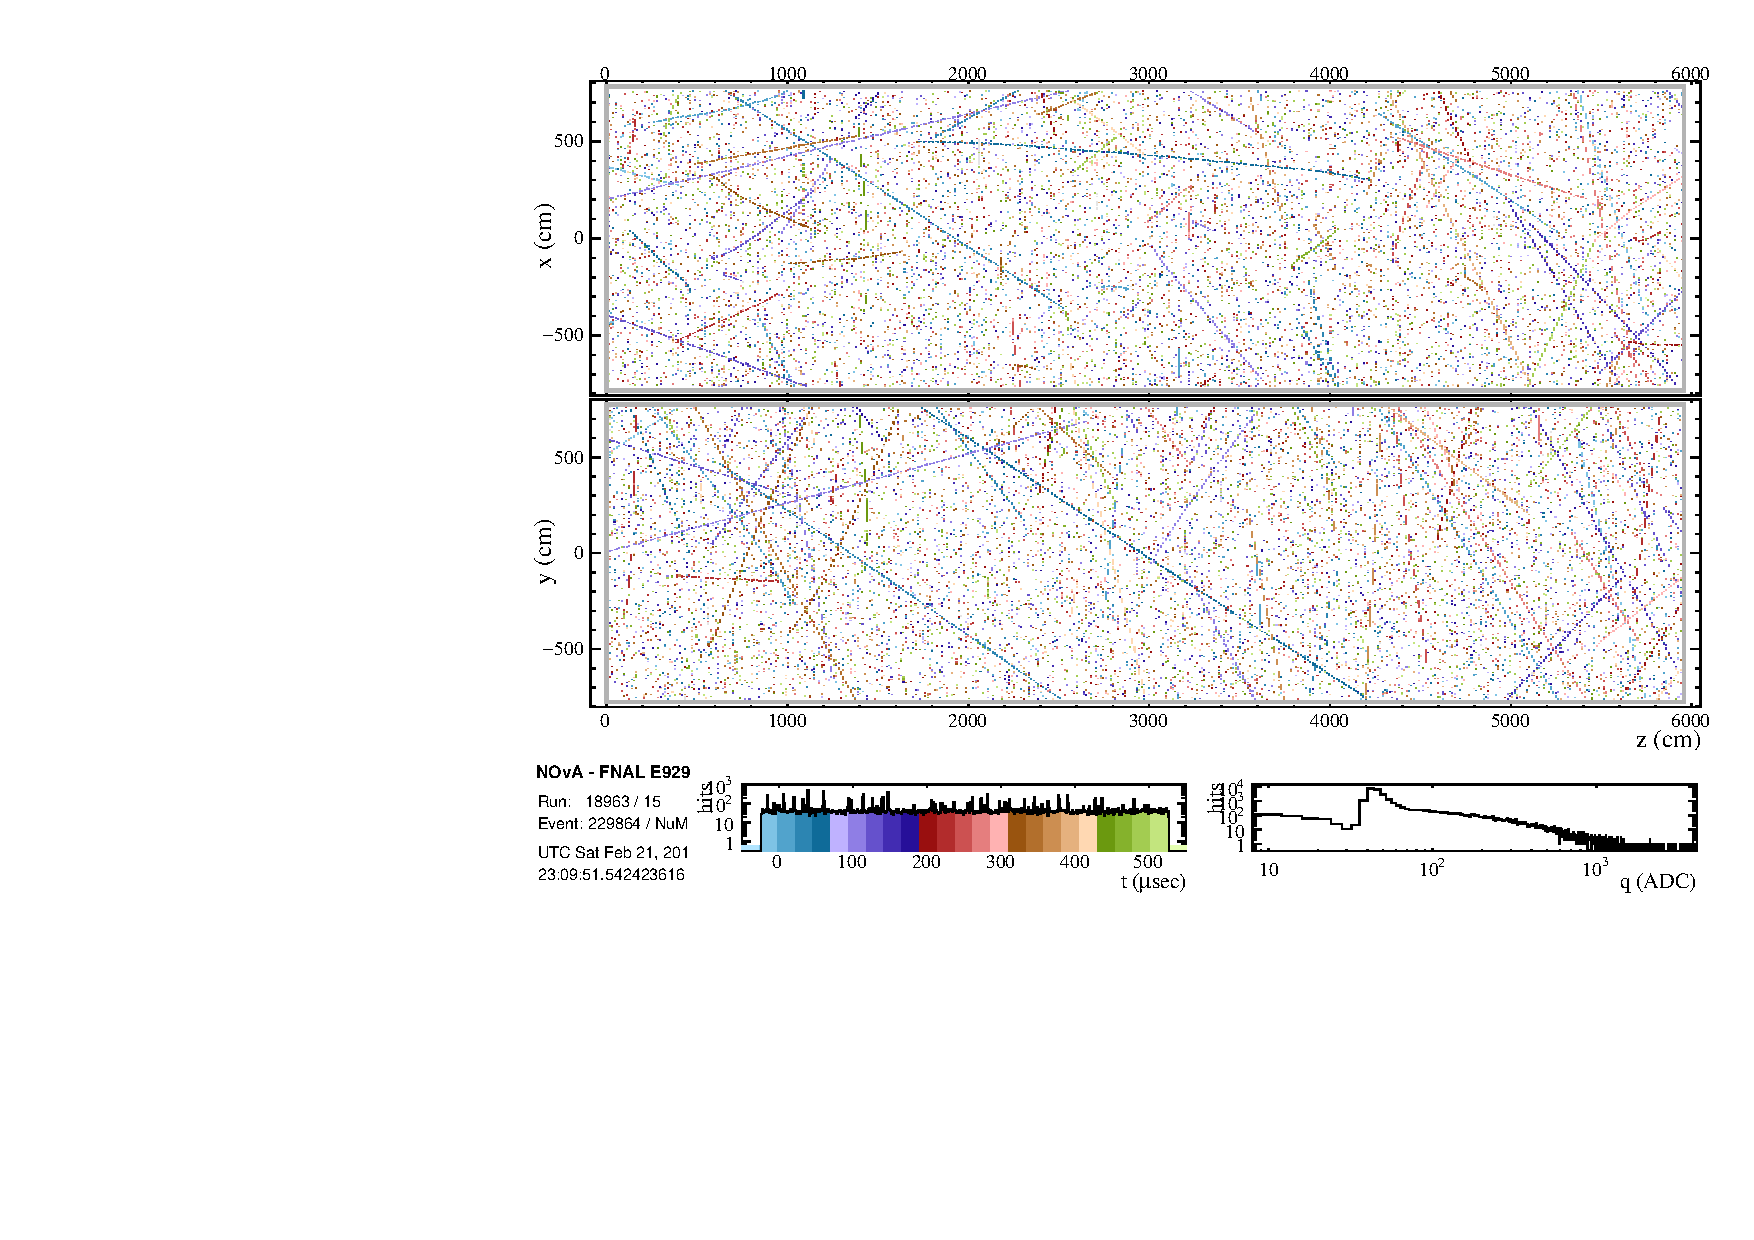
\includegraphics[height=\textwidth, angle=-90]{figures/evd_steps/evd_hits.pdf}

\column{0.5\textwidth}
\centering
\textcolor{custom_red}{After Slicing}
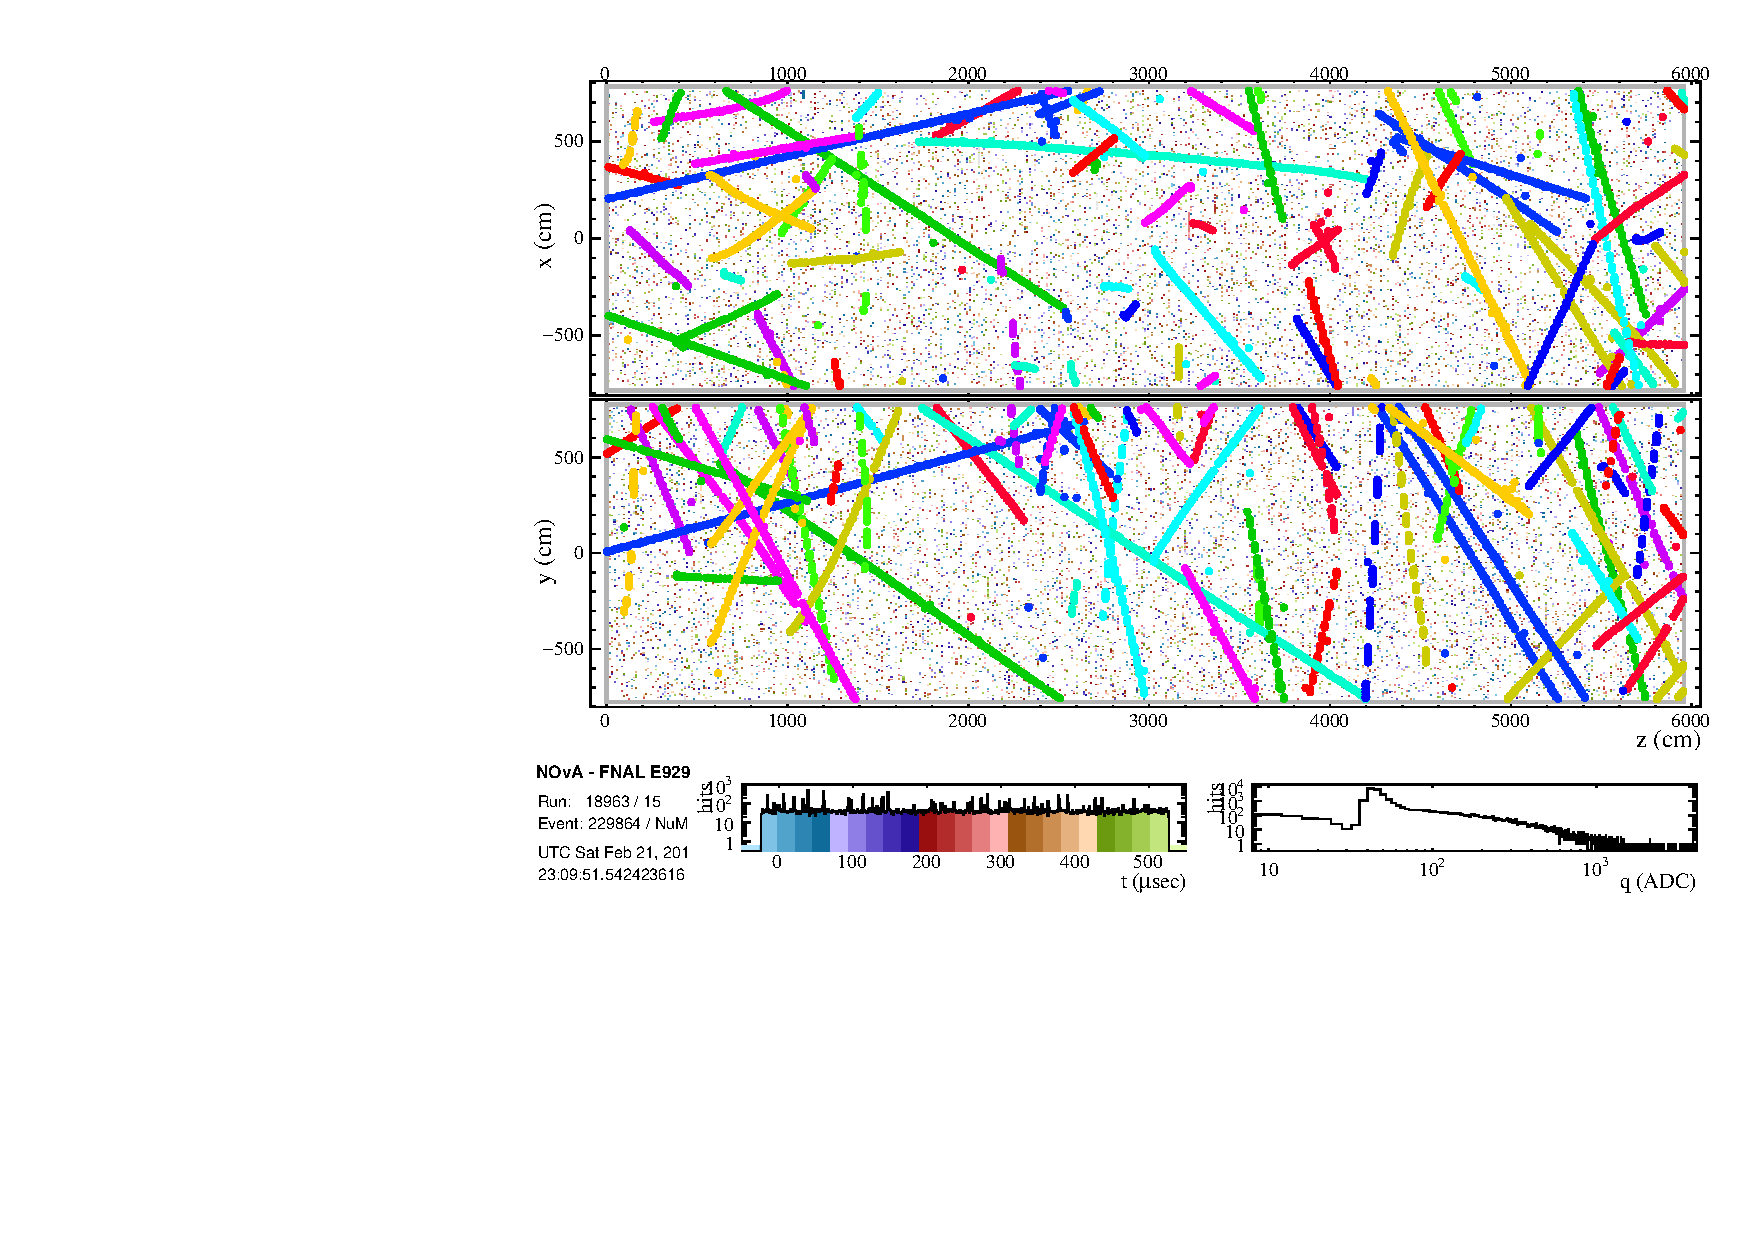
\includegraphics[height=\textwidth, angle=-90]{figures/evd_steps/evd_slice.pdf}

\end{columns}

\end{frame}

\begin{frame}

\frametitle{Reconstruction}
\framesubtitle{Tracking}

\begin{itemize}
\item Tracking locates discrete particle trajectories
\end{itemize}
\gap
\gap
\gap
\begin{columns}[c]
\column{0.35\textwidth}
\centering
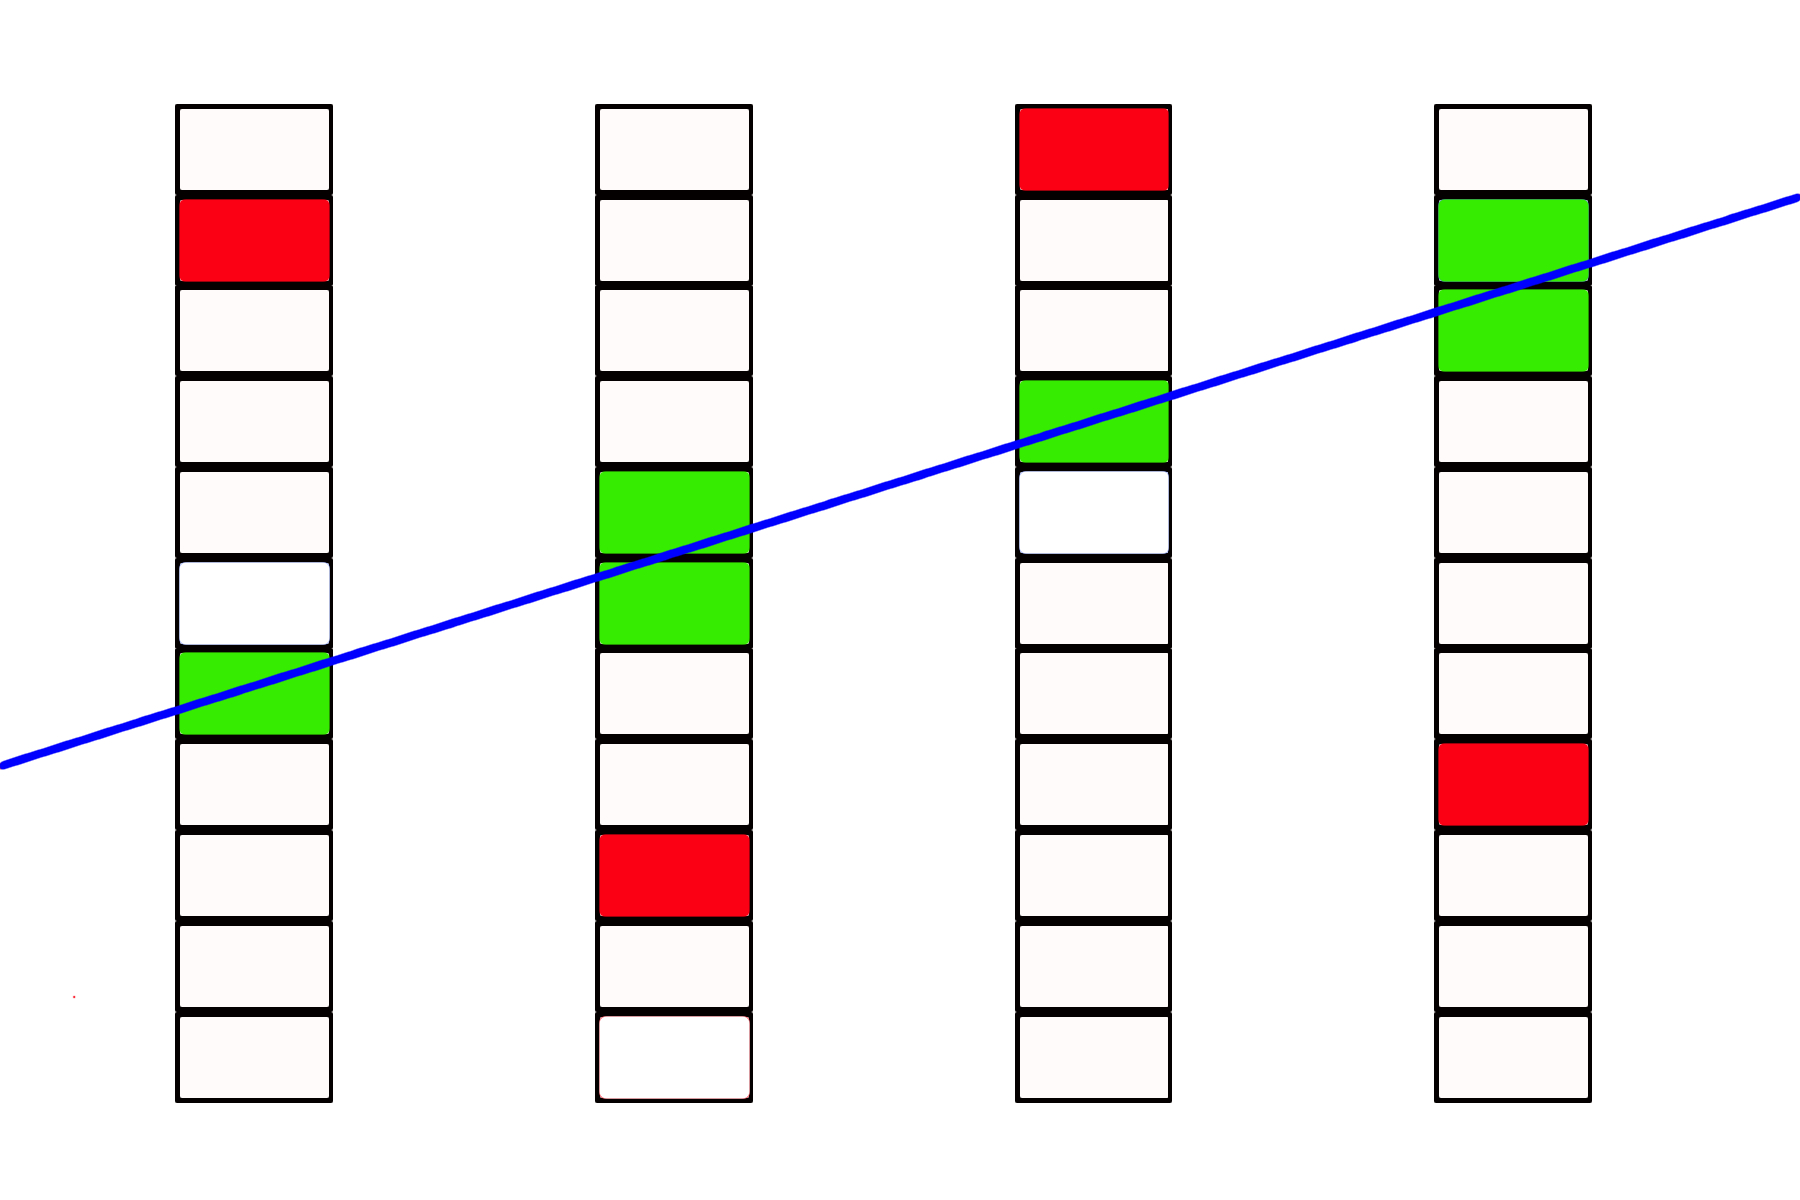
\includegraphics[width=\textwidth]{figures/figures/tracking.jpg}

\column{0.65\textwidth}
\centering
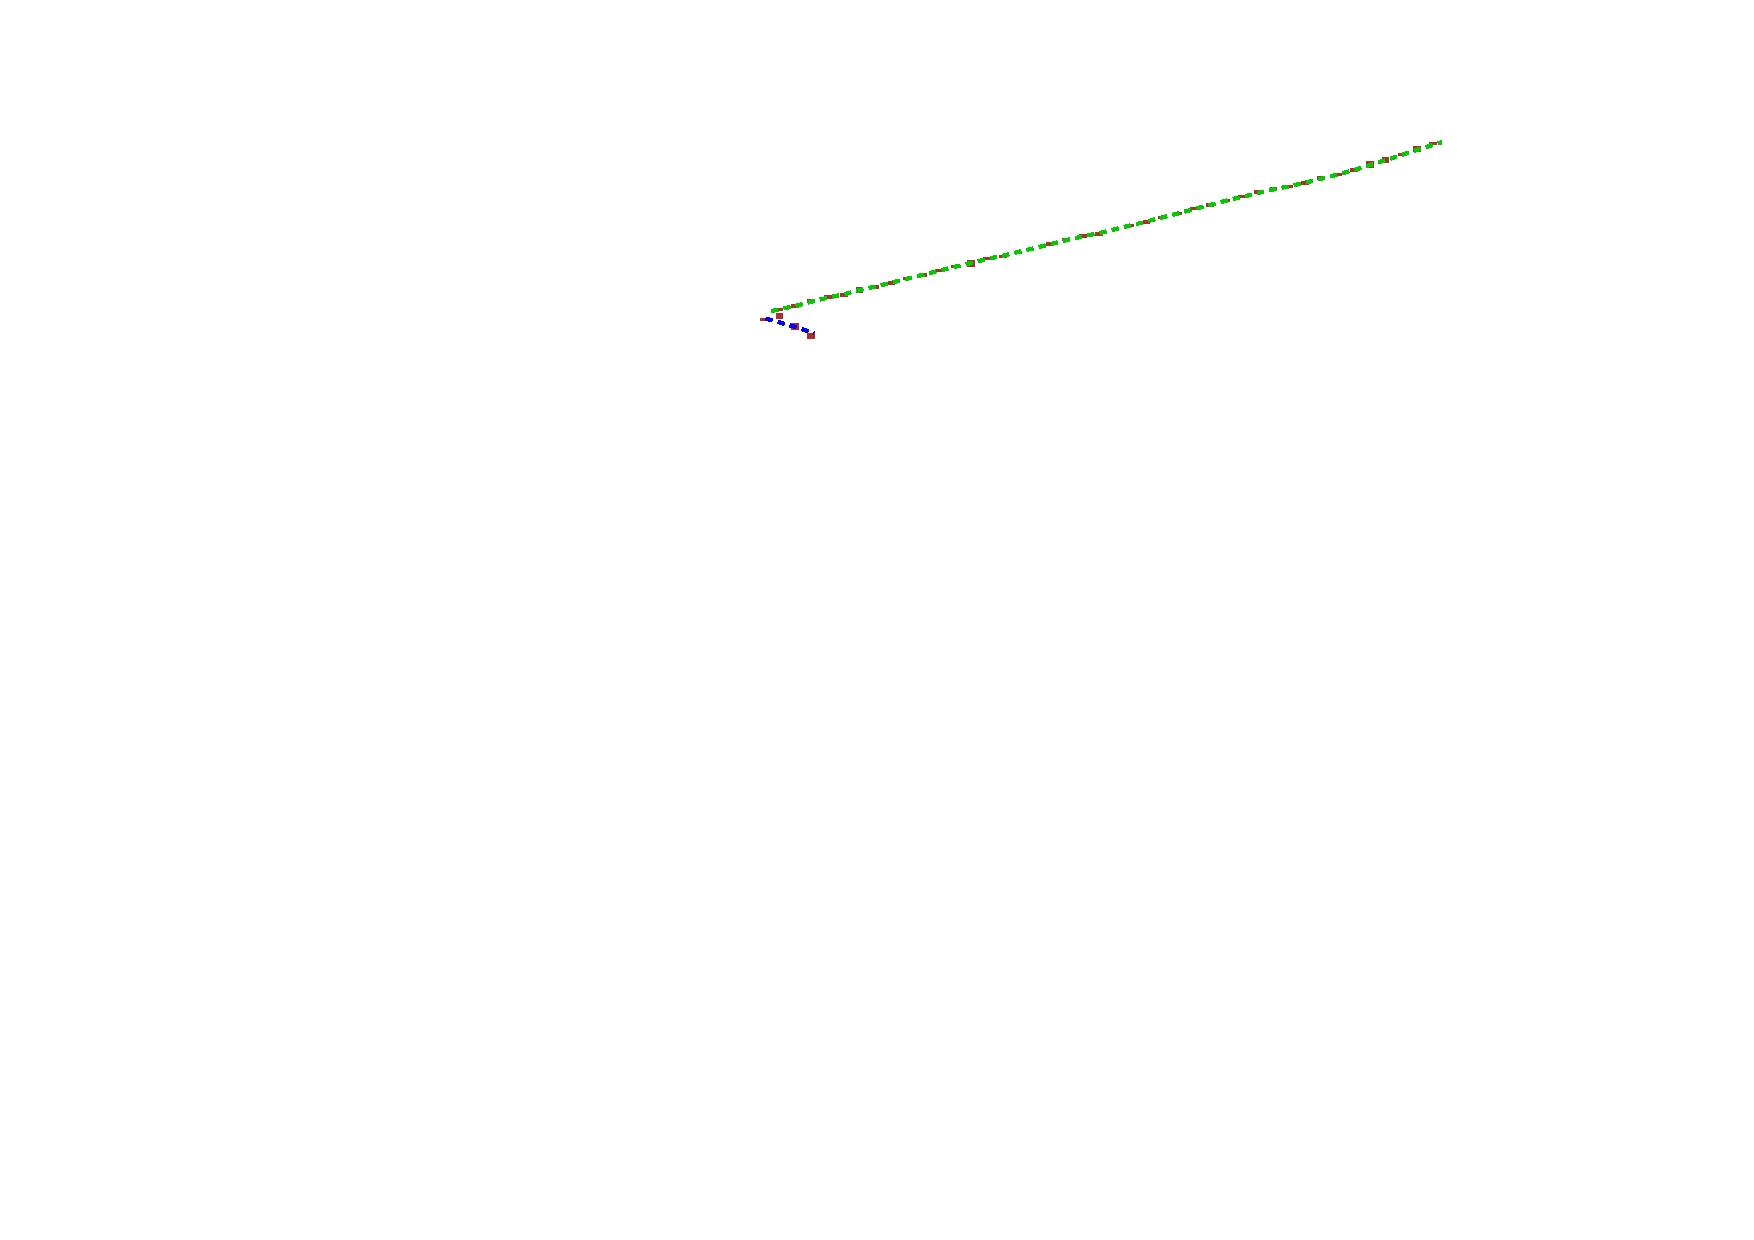
\includegraphics[height=\textwidth, angle=-90]{figures/evd_steps/evd_track_zoom.pdf}

\end{columns}

\end{frame}


\begin{frame}

\frametitle{Reconstruction}
\framesubtitle{Prongs}
\begin{columns}[c]
\column{0.5\textwidth}
  \begin{itemize}
  \item Prongs are for fuzzier trajectories
  \gap
  \item Primary lines are found
  \gap
  \item Vertex located using primary lines
  \gap
  \item Prongs clustered in angular space around vertex

  \end{itemize}
\column{0.5\textwidth}

\centering

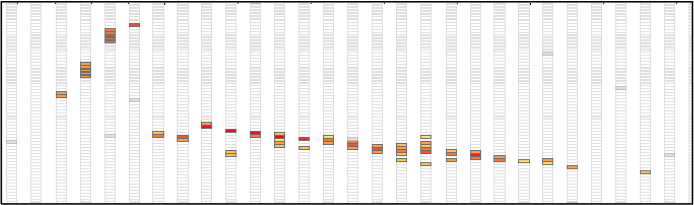
\includegraphics[width=\textwidth]{figures/evd_steps/slice.png}

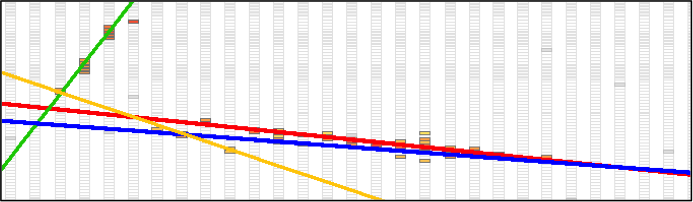
\includegraphics[width=\textwidth]{figures/evd_steps/hough.png}

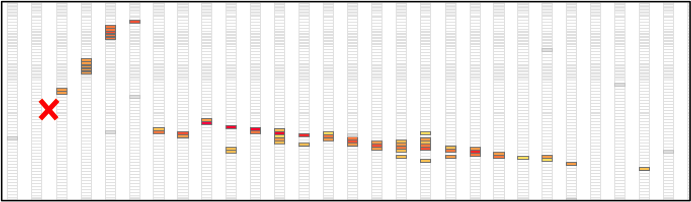
\includegraphics[width=\textwidth]{figures/evd_steps/vertex.png}

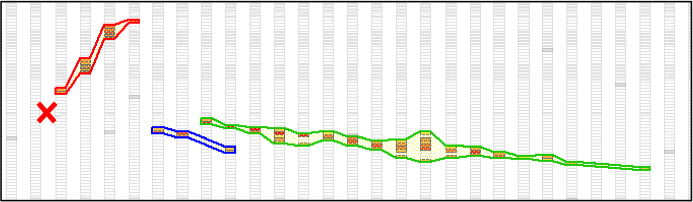
\includegraphics[width=\textwidth]{figures/evd_steps/prongs.png}

\end{columns}


\end{frame}



\begin{frame}

\frametitle{Reconstruction}
\framesubtitle{Muon ID}
\begin{columns}[c]
\column{0.55\textwidth}
  \begin{itemize}
  \item Muons tracks can be identified
  \gap
  \item Features are extracted from tracks
    \begin{itemize}
    \item Track length
    \item Energy deposition characteristic
    \item Scattering characteristic
    \end{itemize}
  \gap
  \item Muon ID score from k-Nearest Neighbors algorithm (machine learning)
  \end{itemize}
\column{0.45\textwidth}

\centering

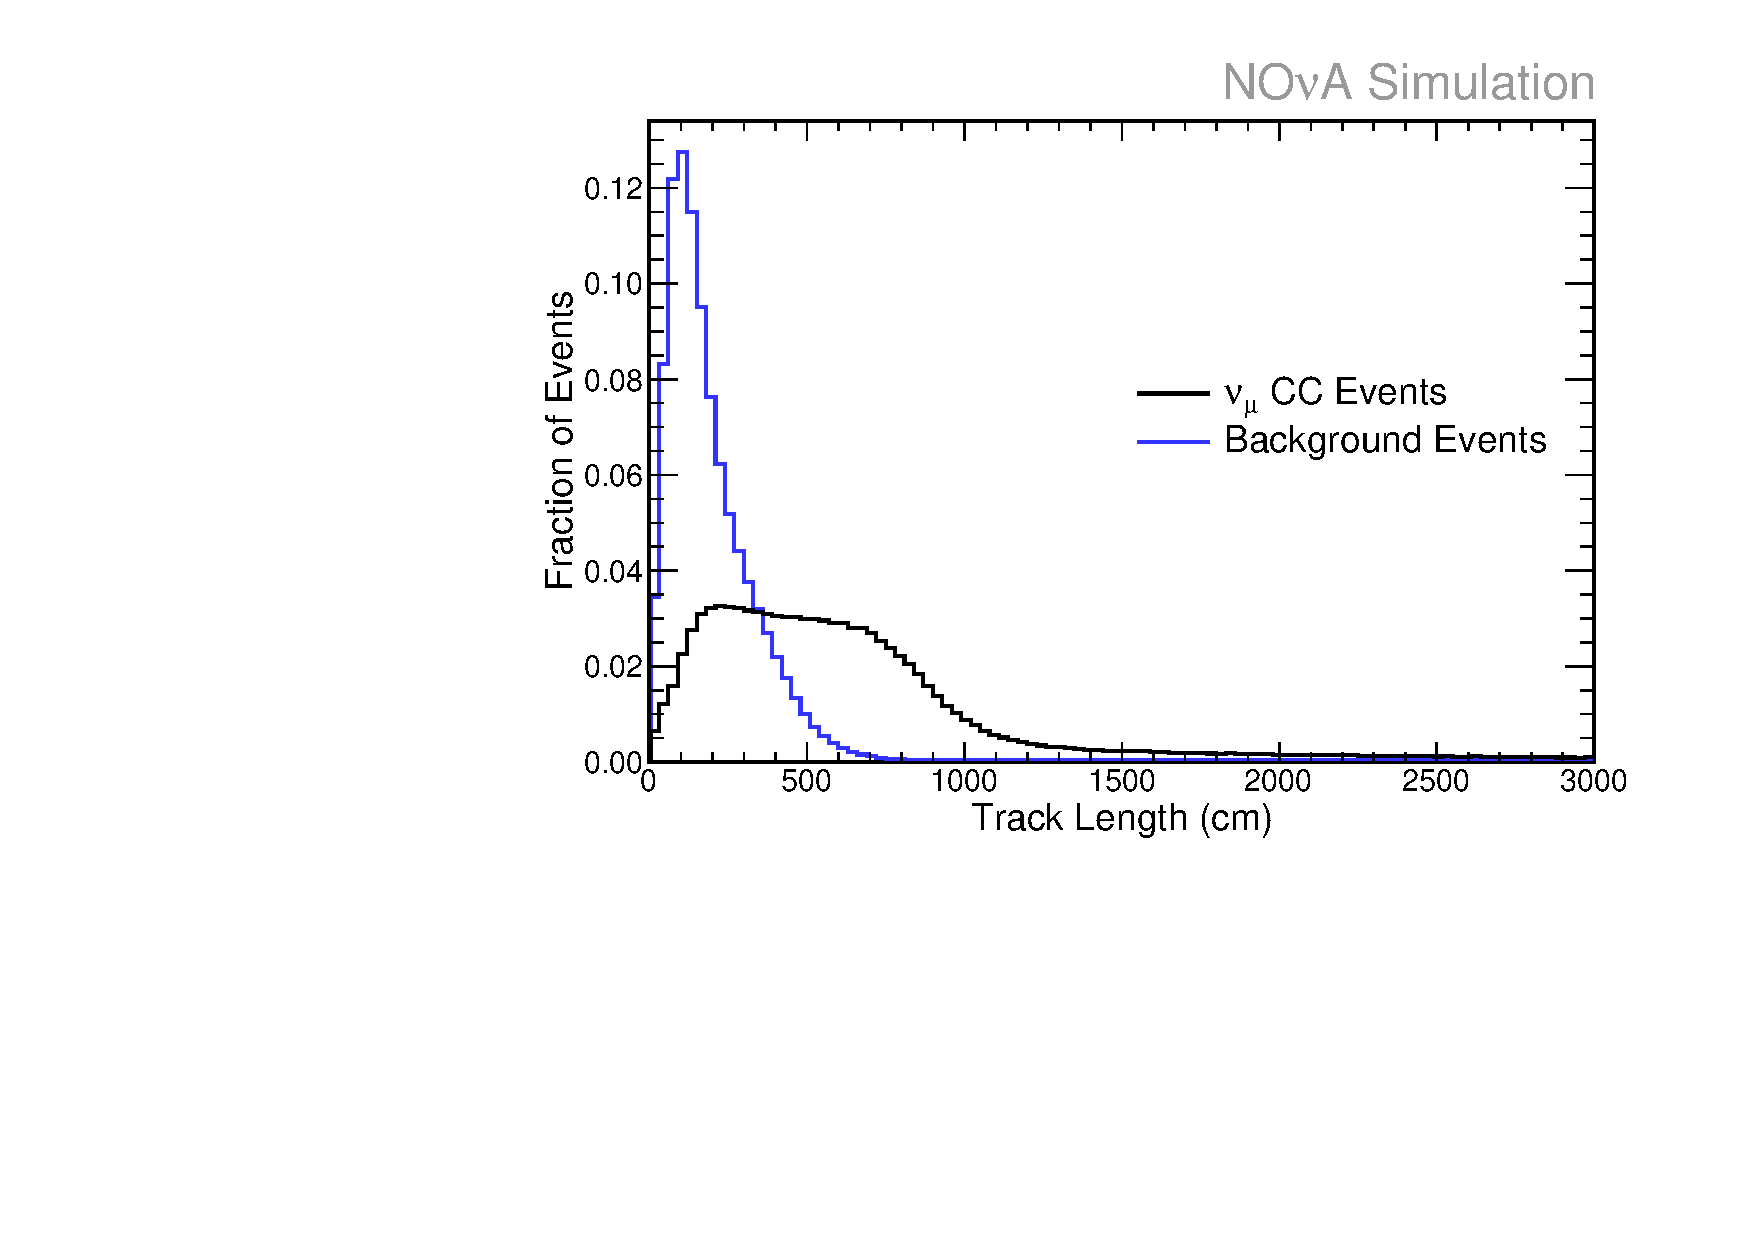
\includegraphics[height=\textwidth, angle=-90]{figures/plots/reco/remid_trk_len.pdf}

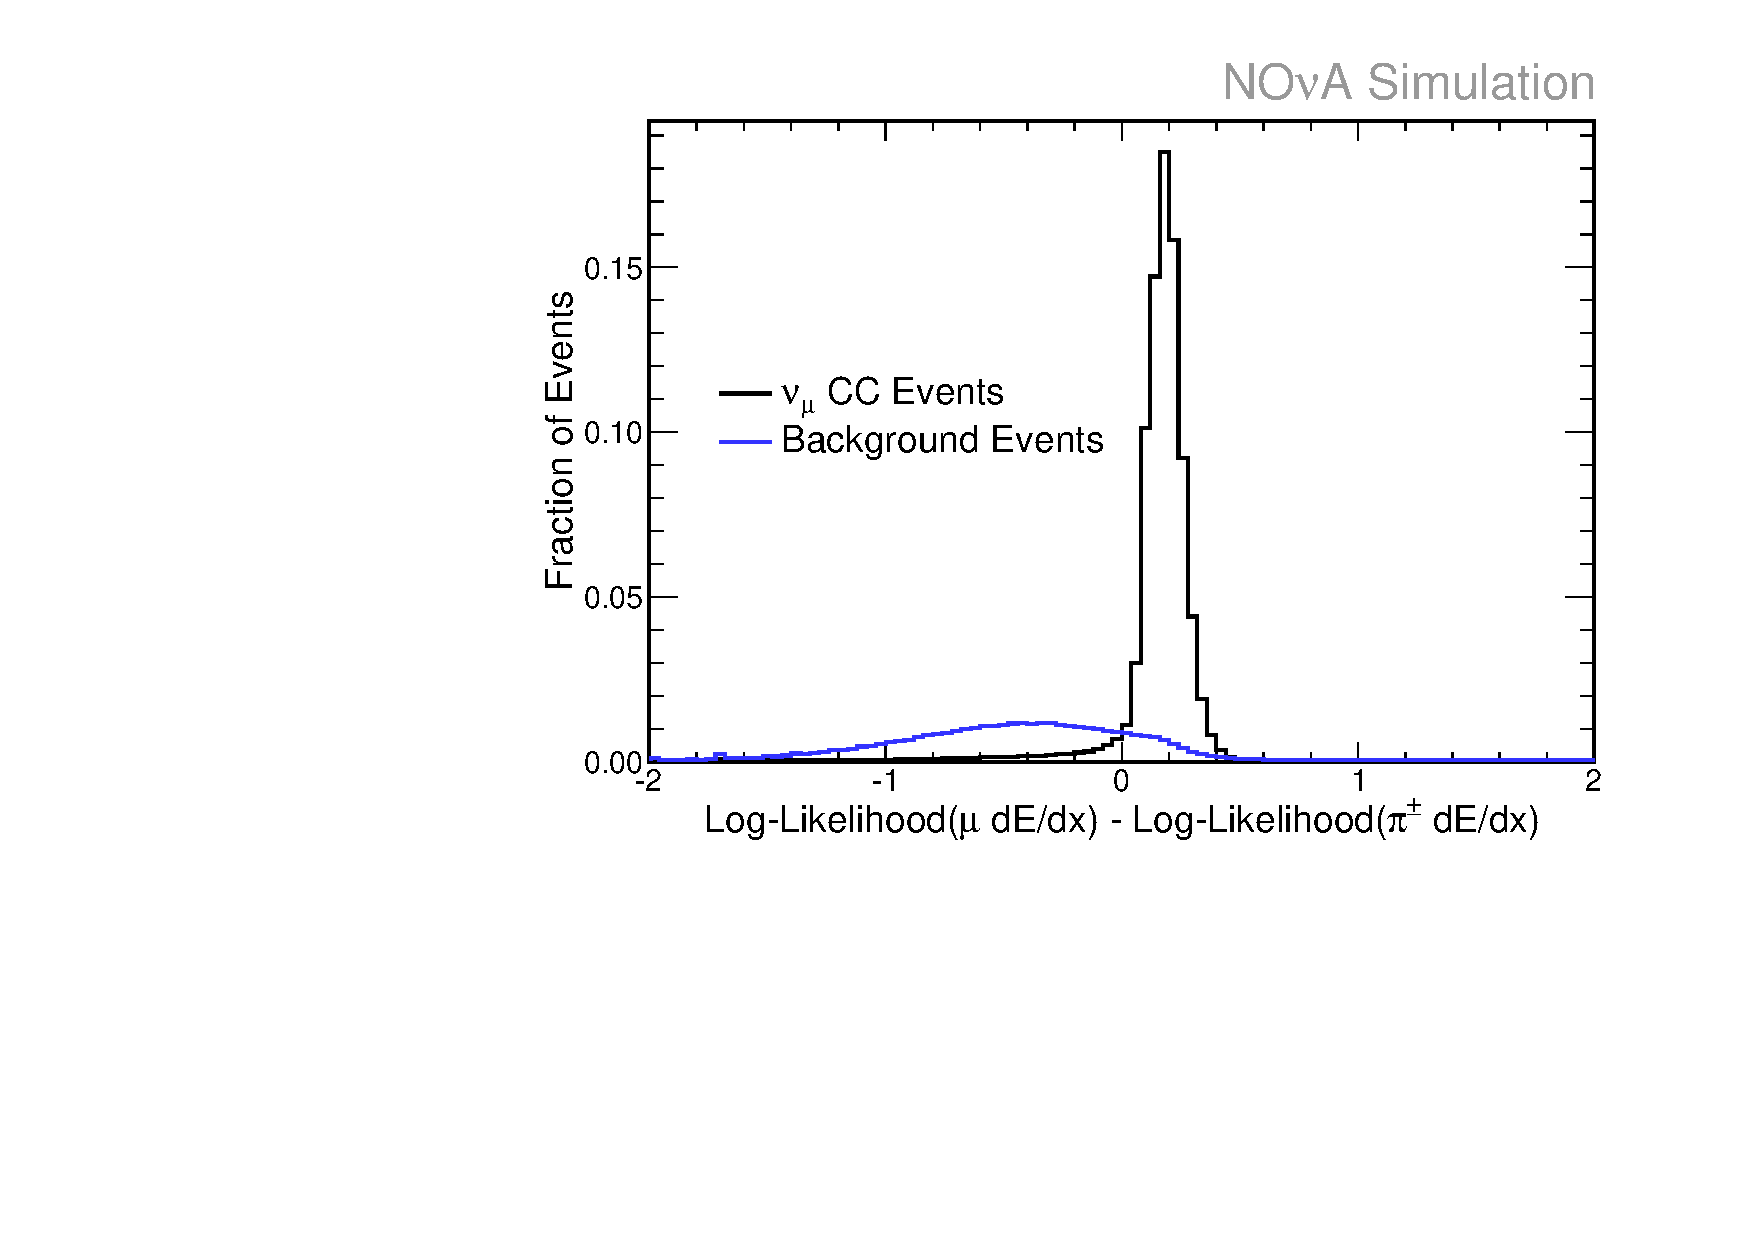
\includegraphics[height=\textwidth, angle=-90]{figures/plots/reco/remid_dedxll.pdf}

\end{columns}


\end{frame}


\begin{frame}
\frametitle{Energy Estimation}
\begin{columns}[c]
\column{0.55\textwidth}
  \begin{itemize}
  \item \numu CC: muon track + hadron shower
  \gap
  \item Muon energy from track length
  \gap
  \item Hadronic energy from remaining visible energy

  \end{itemize}
\column{0.45\textwidth}

\centering

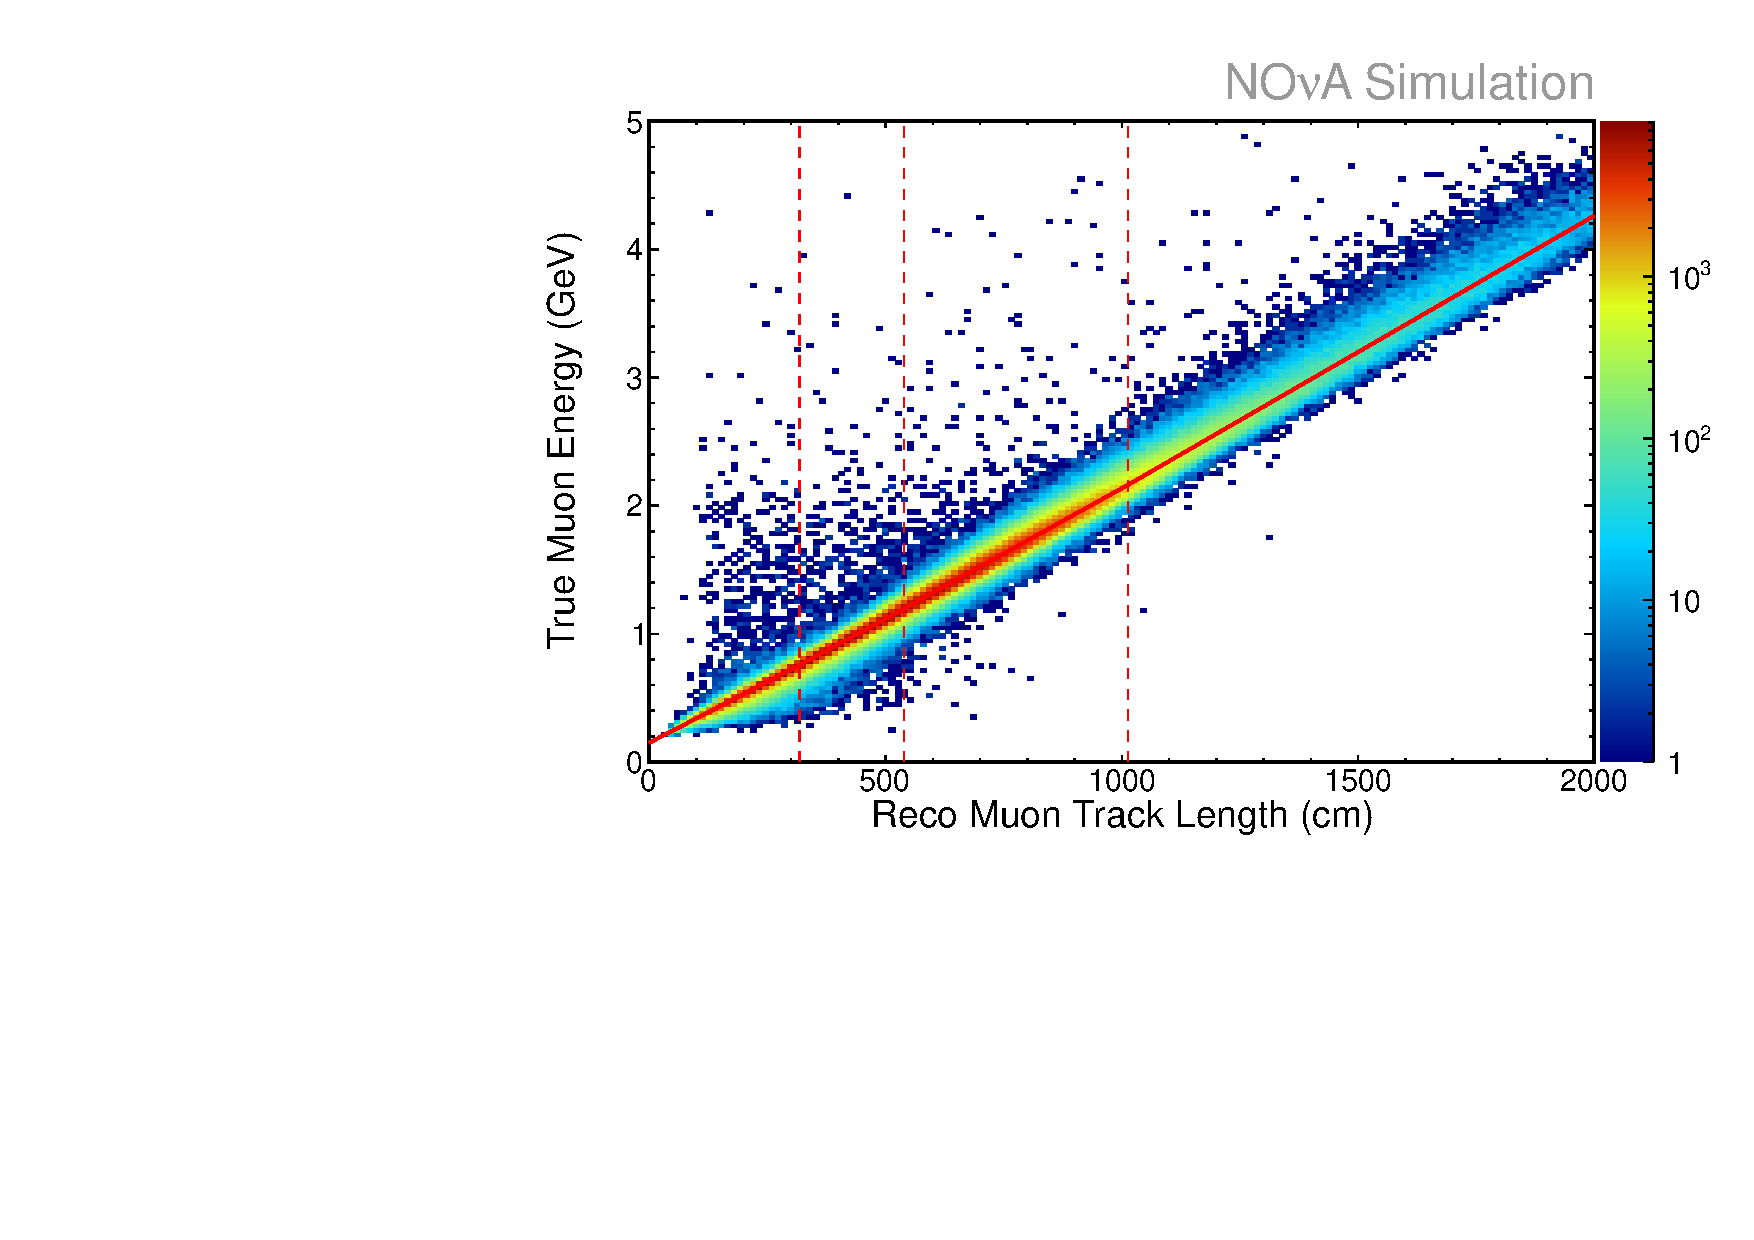
\includegraphics[height=\textwidth, angle=-90]{figures/plots/reco/numu_energy_muon_fit.pdf}

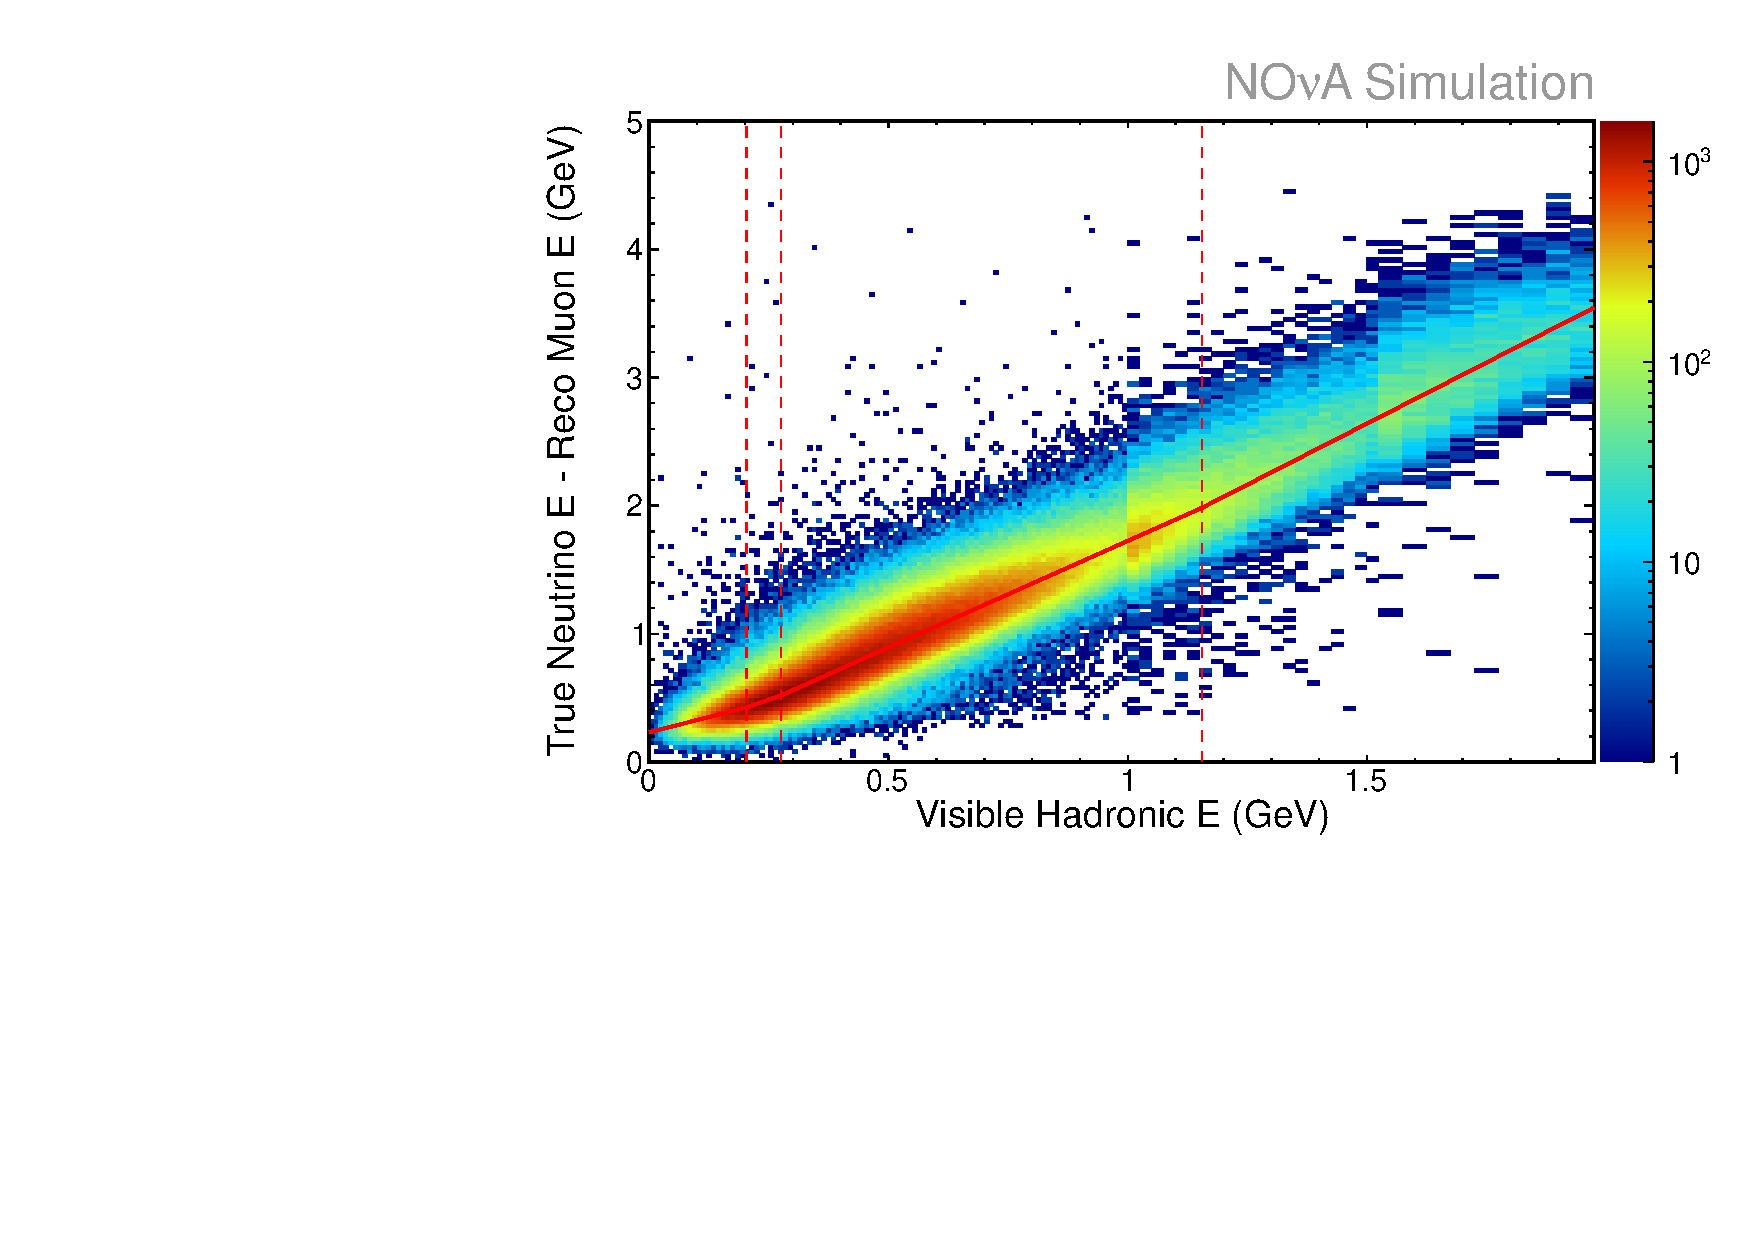
\includegraphics[height=\textwidth, angle=-90]{figures/plots/reco/numu_energy_had_fit.pdf}

\end{columns}


\end{frame}

\begin{frame}
\app{Event Selection (\textit{noun})}{Identification of interaction events which display some physics signal \\
\gap
e.g. \textit{Tony selected \numu charged-current interactions from heaps of background for his \numu disappearance analysis.}}
\end{frame}



\begin{frame}
\frametitle{Event Classification and Selection}

\begin{itemize}
\item Goal: analyze \numu charged-current (CC) interaction events
\gap
\item Two primary sources of background must be minimized
  \begin{itemize}
  \item Cosmic rays
  \item Other $\nu$ interactions from beam, i.e. NC and \nue CC
  \end{itemize}
\end{itemize}
\end{frame}

\begin{frame}
\frametitle{Event Classification and Selection}

\begin{itemize}
\item Traditionally, classification is achieved using reconstructed features
   \begin{itemize}
  \item Criteria based on track length and other characteristics (e.g. Muon ID)
  \item Or, apply machine learning with those features
  \end{itemize}
\gap
\item But perfect reconstruction is difficult!
\gap
\item Using raw detector output could be more robust
\end{itemize}
\end{frame}


\begin{frame}
\frametitle{\nova Events as Images}

\begin{columns}[b]
\column{0.5\textwidth}

\centering
\begin{itemize}
\item \nova events are just images
  \begin{itemize}
  \item[] (two really, $X$-view and $Y$-view)
  \end{itemize}
\gap
\item Discrete pixels
\gap
\item Grayscale intensity
\end{itemize}
\vspace{20pt}
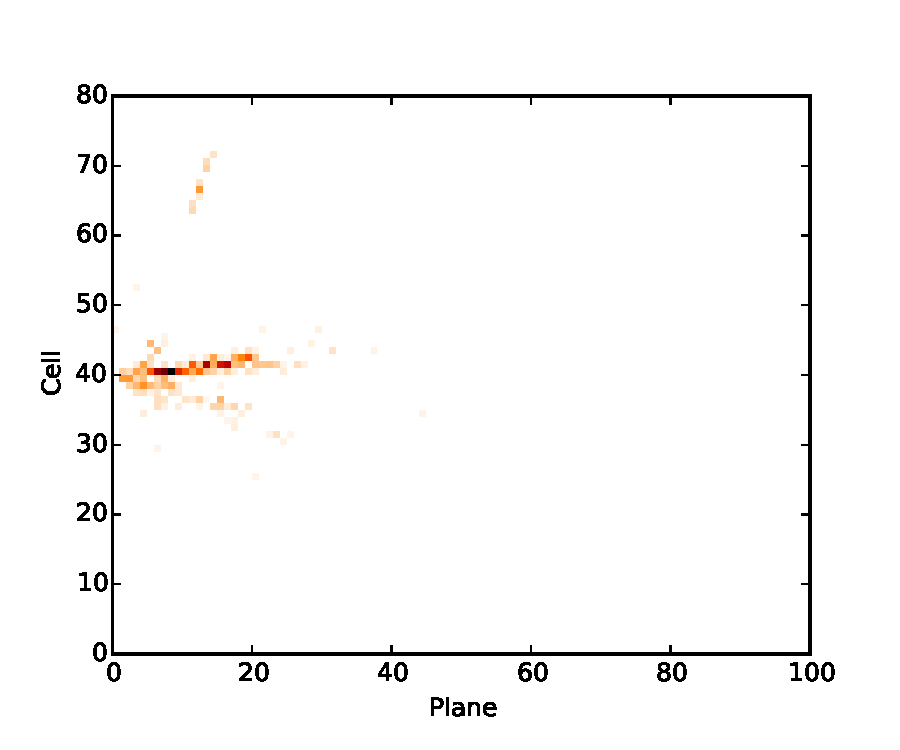
\includegraphics[width=0.85\textwidth]{figures/cnn/view_truetype6_caltype6_event155_x.pdf}


\column{0.5\textwidth}
\centering
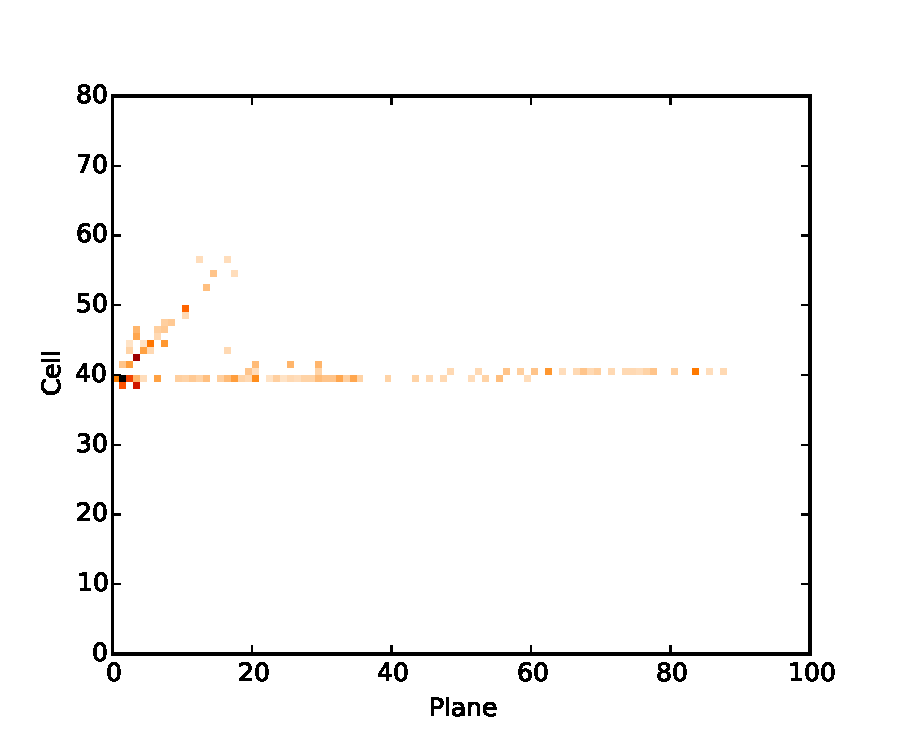
\includegraphics[width=0.85\textwidth]{figures/cnn/view_truetype2_caltype2_event274_x.pdf}

\vspace{-5pt}


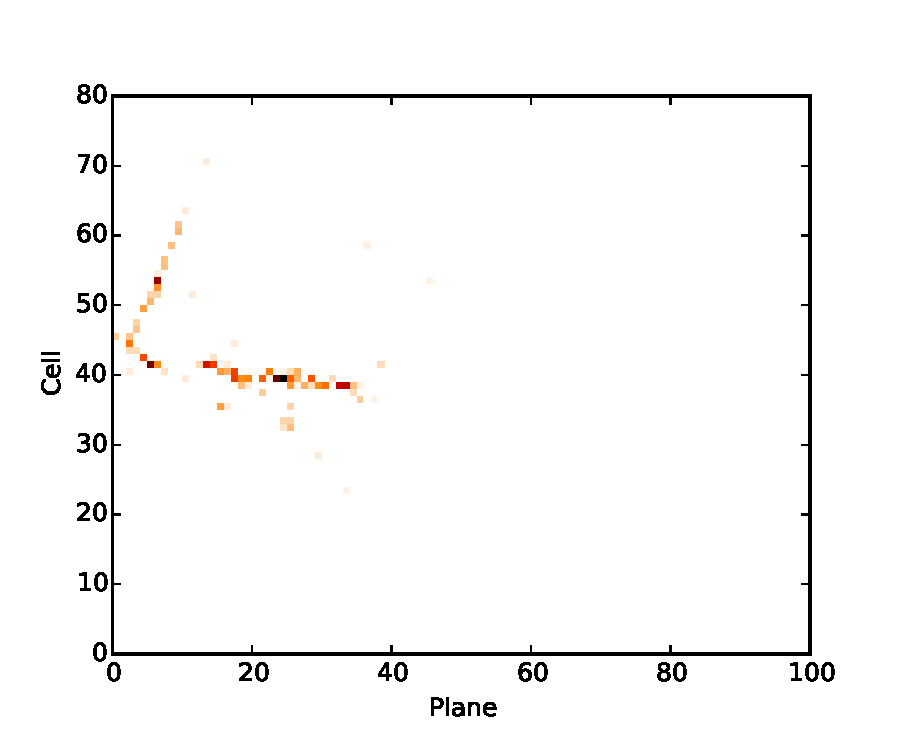
\includegraphics[width=0.85\textwidth]{figures/cnn/view_truetype13_caltype6_event144_x.pdf}

\end{columns}
\end{frame}


\begin{frame}
\frametitle{Neural Networks}

\begin{itemize}
\bang A neural network is a ``feedforward graph" of layers
  \begin{itemize}
  \item Each node, receives input \textit{only} from nodes in previous layers

  \end{itemize}
\gap
  \item Input layer: Example data to be classified
  \item Hidden layers: do the classification
  \item Output layer: classification result

\end{itemize}
\vspace{30pt}
\begin{columns}[c]
\column{0.5\textwidth}

  \begin{itemize}
  \item Supervised learning: network trained using labeled examples
  \gap
  \item ``Backpropagation": gradient-based minimization
    \begin{itemize}
    \item Network parameters are iteratively adjusted to minimize error
    \end{itemize}
  \end{itemize}
\column{0.5\textwidth}
\begin{columns}[c]
\column{0.3\textwidth}
\centering \footnotesize
Input Layer
\column{0.3\textwidth}
\centering \footnotesize
Hidden Layer
\column{0.3\textwidth}
\centering \footnotesize
Output Layer
\end{columns}
\centering
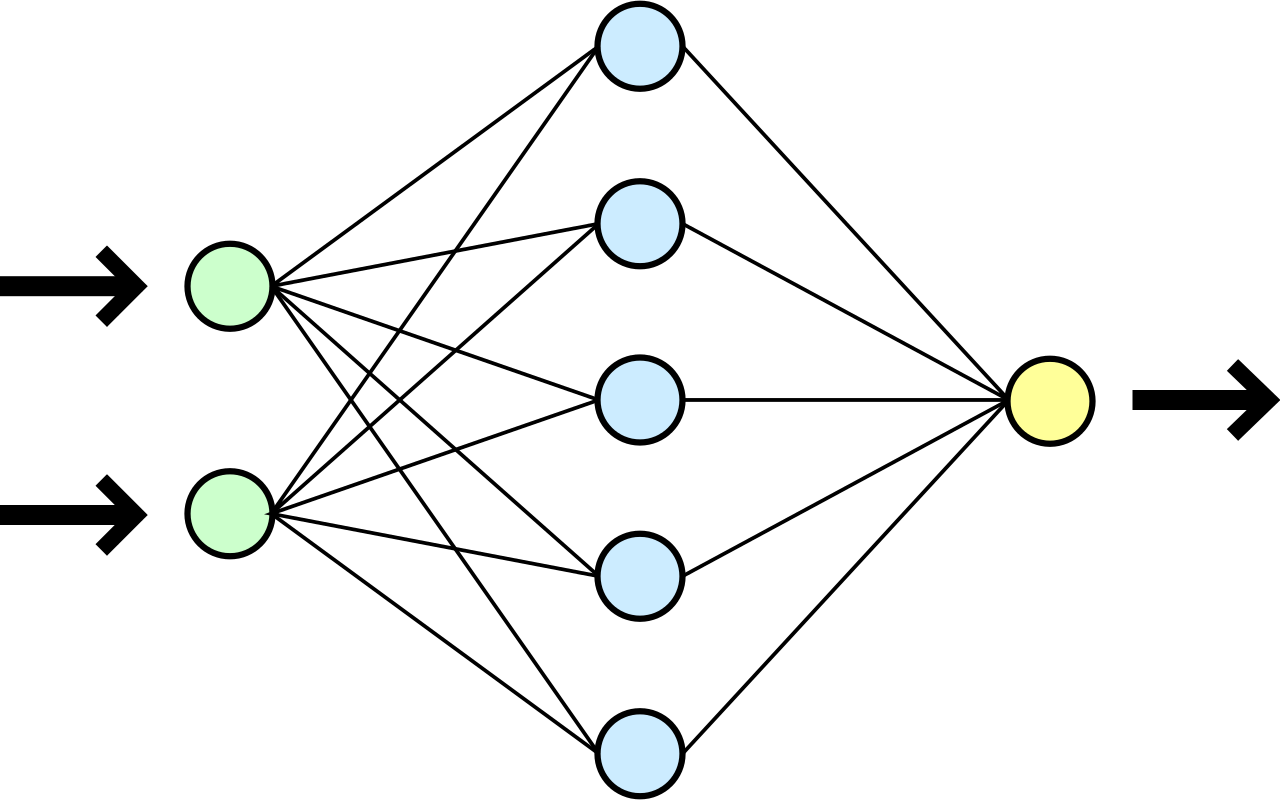
\includegraphics[width=1\textwidth]{figures/figures/basicNN.png}
\end{columns}


\end{frame}


\begin{frame}
\frametitle{Neural Networks}
  \begin{itemize}
  \bang Artificial neural networks (ANN) do well for classification of small images
    \begin{itemize}
    \item e.g. optical character recognition (OCR)
    \end{itemize}
  \end{itemize}
\begin{center}
  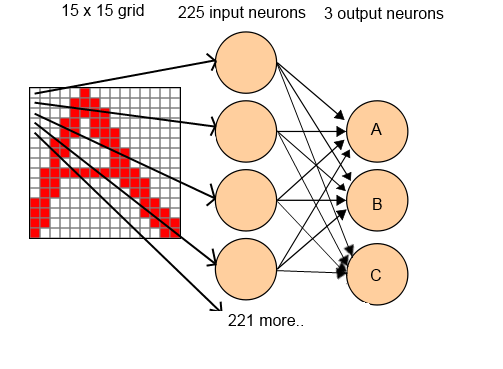
\includegraphics[width=0.6\textwidth]{figures/figures/ocr_ann.png}
\end{center}
\begin{itemize}
    \item But this doesn't scale well above $\sim100$ pixels

\end{itemize}

\end{frame}

\begin{frame}
\frametitle{Neural Networks}

  \begin{itemize}
  \item Image processing community harnessing new technology
    \begin{itemize}
    \item Convolutional neural networks: good for images
    \item New training strategies: deeper networks, less overtraining
    \item GPU acceleration
    \end{itemize}
  \end{itemize}

\end{frame}

\begin{frame}
\frametitle{Convolutional Layers}


  \begin{itemize}
  \item Convolutional layers work well for image classification
  \end{itemize}
  \begin{columns}[c]
  \column{0.5\textwidth}
  \centering 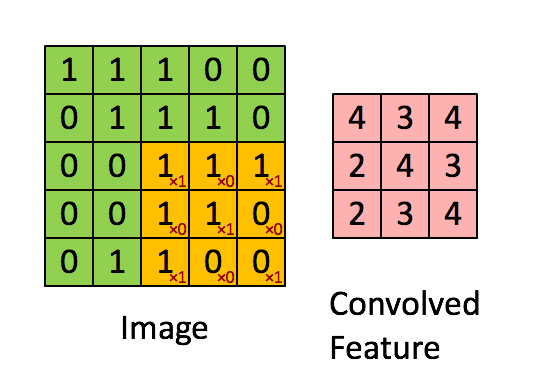
\includegraphics[width=0.7\textwidth]{figures/figures/conv.png}
  \column{0.5\textwidth}
  \centering 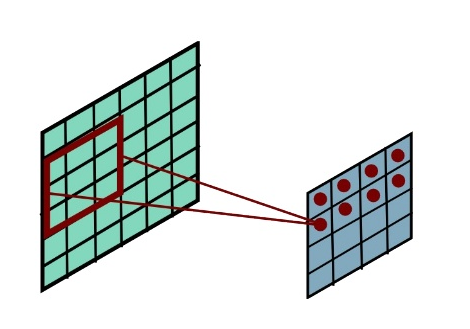
\includegraphics[width=0.7\textwidth]{figures/figures/conv3d.png}
  \end{columns}
  \begin{itemize}
  \gap
  \item Convolutional filters are trained to find features in patches of the image
  \gap
  \item Filters are scanned over the input image to produce a feature map
    \begin{itemize}
    \item Upshot: position independent feature extraction
    \end{itemize}
  \gap
  \end{itemize}

\end{frame}

\begin{frame}
\frametitle{Pooling Layers}
\begin{itemize}
  \item Pooling is a common down-sampling technique
\gap
  \item ``Max pooling" extracts the maximum filter output from each patch
\end{itemize}
\gap
\gap
\centering
 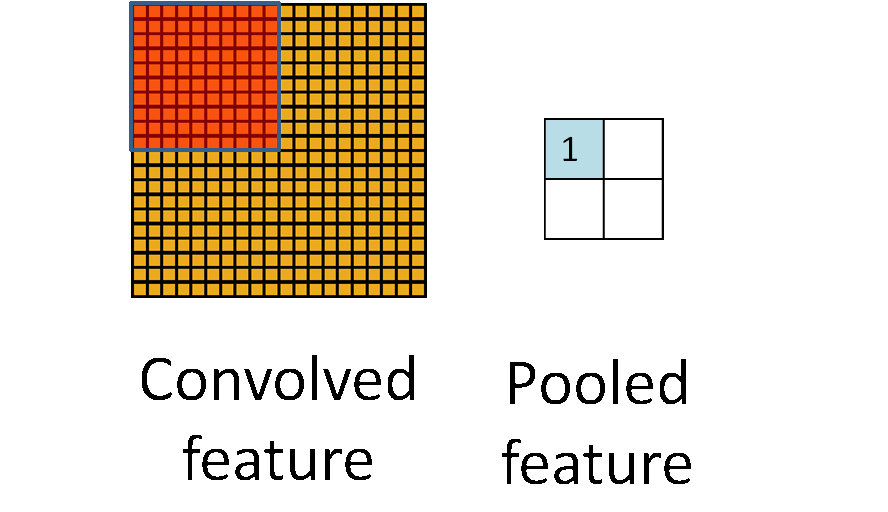
\includegraphics[width=0.5\textwidth]{figures/figures/pooling.png}
\end{frame}


\begin{frame}
\frametitle{Convolutional Networks}
\begin{itemize}
  \item Many filters trained in a each convolutional layer
  \gap

  \begin{center}
 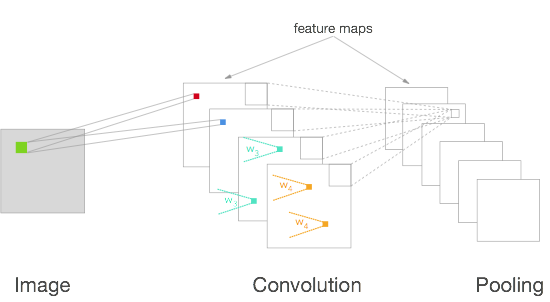
\includegraphics[width=0.8\textwidth]{figures/figures/convnet.png}
 \end{center}

\end{itemize}
\end{frame}

\begin{frame}
\frametitle{GoogLeNet and \textit{Inception}}

  \begin{itemize}
  \item GoogLeNet introduced the ``Inception module"
  \end{itemize}
  \begin{center}
 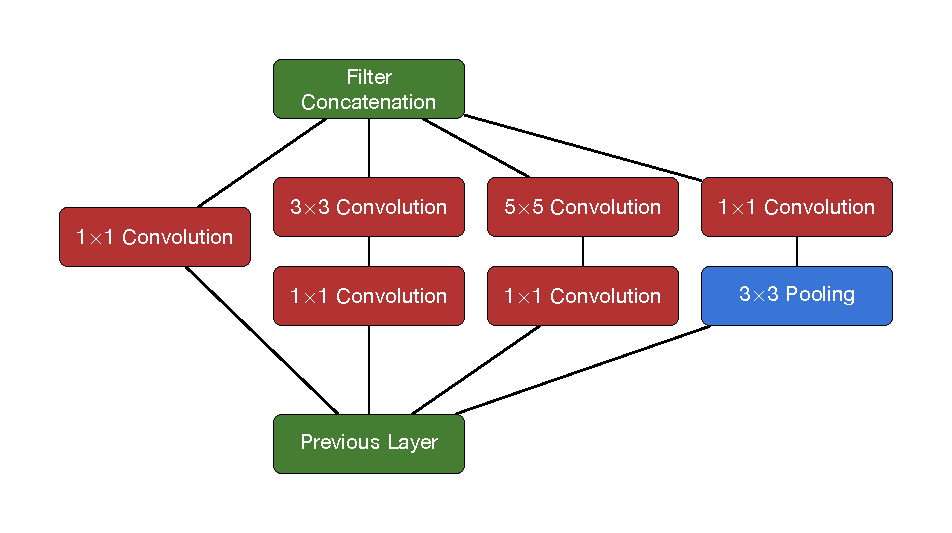
\includegraphics[width=0.6\textwidth]{figures/figures/inception/inception.pdf}
 \end{center}
   \begin{itemize}
  \item Convolutional layers are arranged side-by-side rather one after another
  \item Downstream layers simultaneously learn structure at different scales
  \item $1\times1$ convolution is a tool for dimensionality reduction
    \begin{itemize}
    \item $1\times1$ convolution: constant scale factor
    \item Output filters are linear combinations of input filters
    \end{itemize}
  \end{itemize}

\end{frame}



\begin{frame}

\frametitle{\nova CNN Architecture}

  \begin{columns}
  \column{0.28\textwidth}
   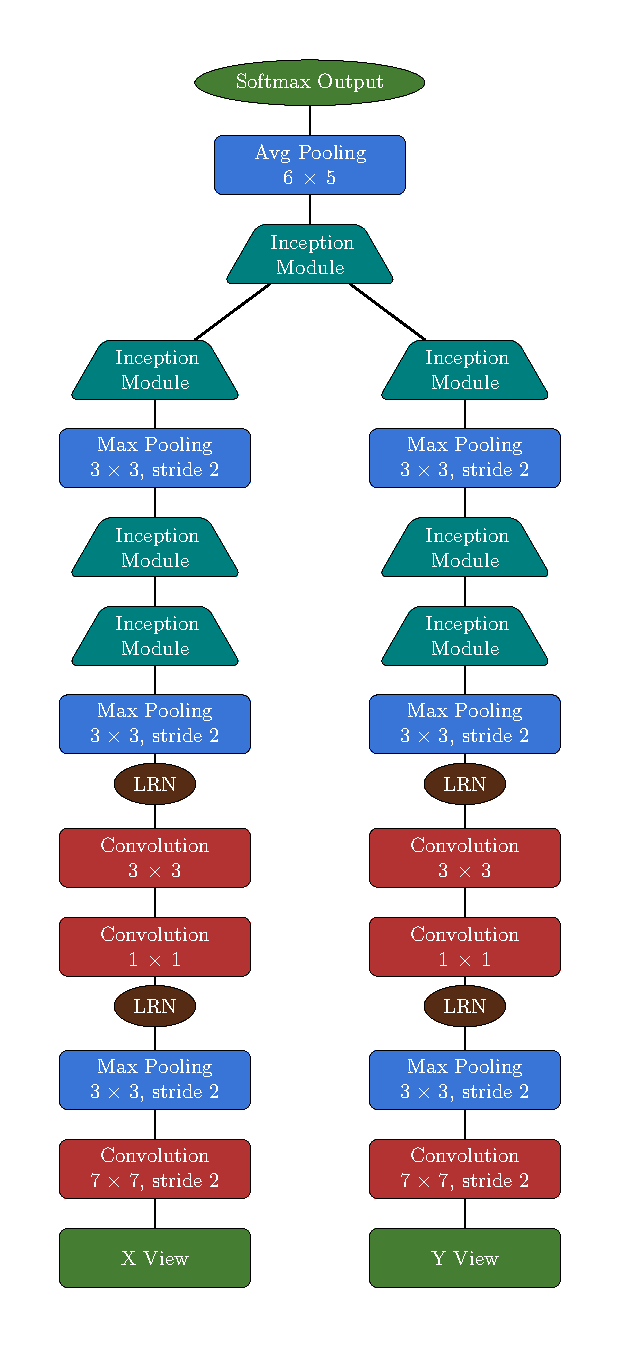
\includegraphics[height=0.95\textheight]{figures/arch/arch.pdf}
  \column{0.72\textwidth}
  \begin{itemize}
  \item Separate branches for $X$ and $Y$ views
  \gap
  \item Repeated convolution, pooling, inception structures
  \gap
  \item Local Response Normalization (LRN) for smoothing
  \end{itemize}
  \end{columns}
\end{frame}

\begin{frame}
\frametitle{CNN Filter}

\begin{itemize}
\item First convolution layer, $7\times7$
\end{itemize}

\begin{columns}[b]
\column{0.45\textwidth}
\centering
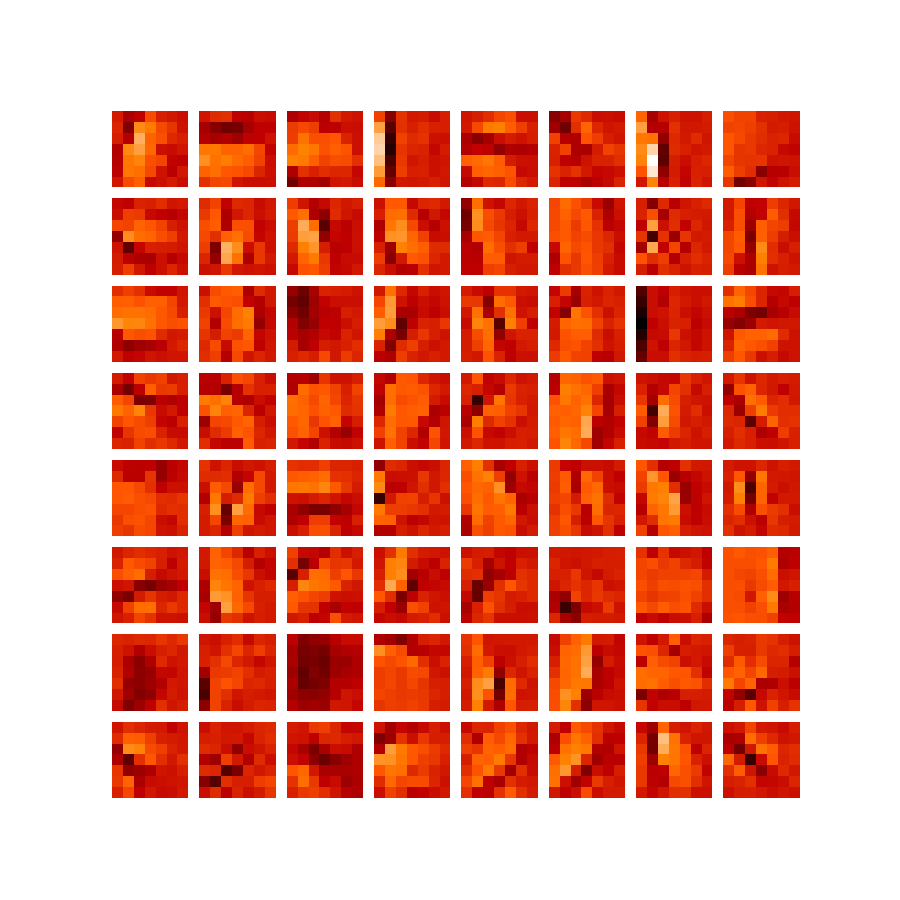
\includegraphics[width=\textwidth]{figures/cnn/conv1y.pdf}

Filters
\column{0.55\textwidth}
\centering
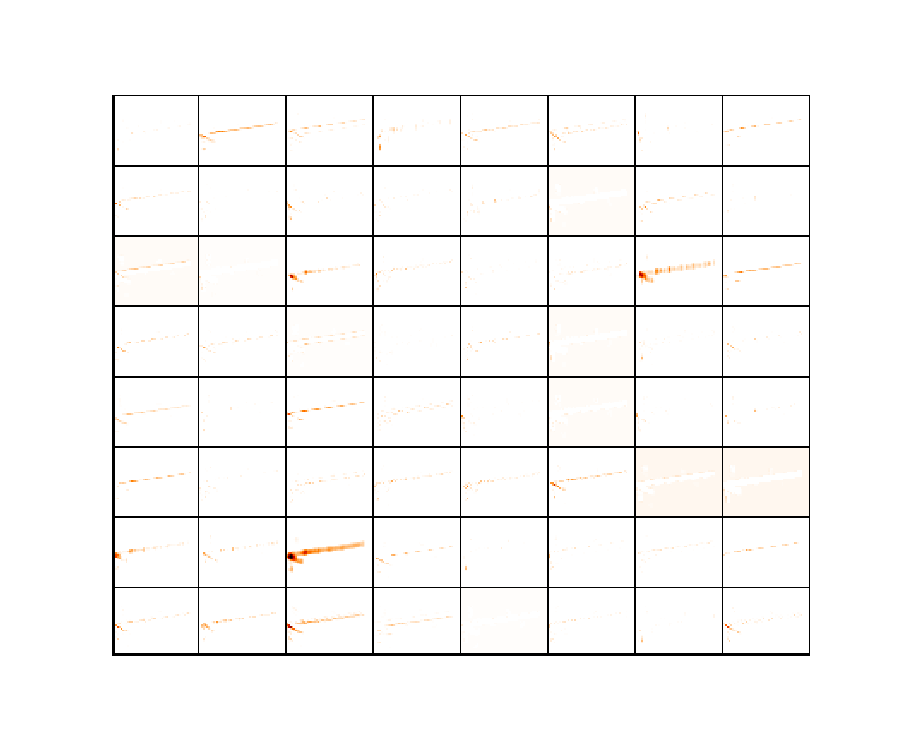
\includegraphics[width=\textwidth]{figures/cnn/feat1_truetype2_caltype2_event274_y.pdf}

Filtered output
\end{columns}

\end{frame}


\begin{frame}
\frametitle{Inception Module Filters}

\begin{columns}[t]

\column{0.5\textwidth}
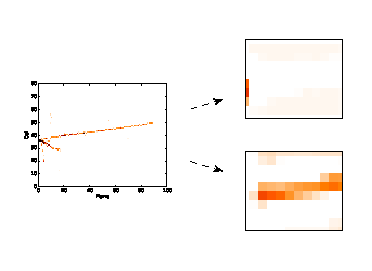
\includegraphics[width=1\textwidth,viewport=10 13 170 115, clip=true]{figures/cnn/featurePlotNuMuDIS}
\gap

\includegraphics[width=1\textwidth,viewport=10 13 170 115, clip=true]{figures/cnn/featurePlotNuMuQE}


\column{0.5\textwidth}
\includegraphics[width=1\textwidth,viewport=10 13 170 115, clip=true]{figures/cnn/featurePlotNC}
\gap
\gap
\begin{itemize}
\item Output from inception module is more discerning
\item Two particular filters in each pane
\item Top finds hadronic shower
\item Bottom finds muon tracks
\end{itemize}


\end{columns}
\end{frame}


\begin{frame}

\frametitle{CNN Softmax Output}

  \begin{center}
\includegraphics[height=0.7\textwidth, angle=-90]{figures/cnn/numu_pid_dist.pdf}

  \end{center}
  \begin{itemize}
  \item Strong discriminant for \numu CC events
  \end{itemize}
\end{frame}


\begin{frame}
\frametitle{Event Selection}

\begin{itemize}
\item Event selection serves two purposes:
  \begin{itemize}
  \item Quality: need sufficient information to estimate energy
  \item Background rejection: need clean sample of \numu CC
  \end{itemize}
\item Containment is important for both purposes
  \begin{itemize}
  \item Events which escape detector have missing energy
  \item Cosmic rays commonly traverse entire detector (i.e. touch edges)
  \end{itemize}
\end{itemize}
\begin{center}
 \includegraphics[width=0.7\textwidth]{figures/selection/cosmicmuons.png}
\end{center}

\end{frame}

\begin{frame}
\frametitle{Event Selection}


\begin{itemize}
\item Events are required to pass a extra few criteria
\begin{itemize}
\item CNN Output
\item CosmicTrack Max-Y
\item Transverse momentum estimated from slice
\item Transverse momentum estimated from prongs

\end{itemize}
\end{itemize}
\end{frame}


\begin{frame}

\frametitle{CNN Output}

  \begin{center}
  \includegraphics[height=0.7\textwidth, angle=-90]{figures/selection/n1_cvnnumu.pdf}

  {\footnotesize(``$n-1$'' histogram -- only events which pass all other criteria)}
  \end{center}
  \begin{itemize}
  \item Select events with CNN output > 0.5
  \end{itemize}
\end{frame}



\begin{frame}
\frametitle{CosmicTrack start $Y$ position}

  \begin{center}
  \includegraphics[height=0.7\textwidth, angle=-90]{figures/selection/n1_cosStartY.pdf}

  {\footnotesize(``$n-1$'' histogram -- only events which pass all other criteria)}
  \end{center}
  \begin{itemize}
  \item Select events with start $Y$ < 6.0 m
  \end{itemize}
\end{frame}


\begin{frame}
\frametitle{Transverse momentum from slice mean}

  \begin{center}
  \includegraphics[height=0.7\textwidth, angle=-90]{figures/selection/n1_tranMom.pdf}

  {\footnotesize(``$n-1$'' histogram -- only events which pass all other criteria)}
  \end{center}
  \begin{itemize}
  \item Select events with $P_T$ < 0.8
  \end{itemize}
\end{frame}

\begin{frame}
\frametitle{Transverse momentum from prongs}

  \begin{center}
  \includegraphics[height=0.7\textwidth, angle=-90]{figures/selection/n1_pngptp.pdf}

  {\footnotesize(``$n-1$'' histogram -- only events which pass all other criteria)}
  \end{center}
  \begin{itemize}
  \item Select events with $P_T$ < 0.8
  \end{itemize}
\end{frame}

\begin{frame}
\frametitle{Selection Comparison}

\begin{columns}
  \column{0.5\textwidth}
  \begin{center}
   \includegraphics[height=\textwidth, angle=-90]{figures/selection/cosmic_sig_osc.pdf}
  \end{center}

  \column{0.5\textwidth}
  \begin{center}
   \includegraphics[height=\textwidth, angle=-90]{figures/selection/cosmic_sig_eff_osc.pdf}
  \end{center}

\end{columns}
\gap
  \begin{itemize}
  \item Existing \nova analysis uses muon ID and boosted decision tree (BDT)
  \gap
  \item New CNN-based selection is more efficient, especially in low energy region
  \end{itemize}
\end{frame}

\begin{frame}
\app{Analysis (\textit{noun})}{Measurement of physical parameters by comparing data and prediction}
\end{frame}


\begin{frame}
\frametitle{Analysis}
\begin{center}
\vspace{-10pt}
\includegraphics[width=.45\textheight, angle=-90]{figures/results/spectrum_fit_systs.pdf}
\end{center}

\begin{itemize}

\item FD spectrum is fit to prediction
\gap
\item Log-likelihood for binned, Poisson distributed data
\end{itemize}
\begin{columns}[c]
\column{0.05\textwidth}
~
\column{0.4\textwidth}
\begin{equation*}
\chi^2 = 2 \sum_i e_i - o_i + \ln \big (\frac{o_i}{e_i} \big)
+ \sum_j \frac{s_j^2}{\sigma_j^2}
\end{equation*}
\column{0.4\textwidth}
  \begin{itemize}
  \item[] ~
  \begin{itemize}
  \item Bins: $i$
  \item Prediction in each bin: $e_i$
  \item Observation in each bin: $o_i$
  \item Systematic uncertainties: $j$
  \item Systematic shifts: $s_j$
  \item Systematic constraint: $\sigma_{ij}$
  \end{itemize}
  \end{itemize}
\end{columns}
\end{frame}

\begin{frame}
\frametitle{Prediction}
\begin{columns}[c]
\column{0.5\textwidth}
\begin{itemize}
\item FD prediction is extrapolated from ND data
\gap
\item ND data controls systematic uncertainties, e.g. flux
\gap
\item ND and FD spectra are not identical (geometric effects)
\end{itemize}
\column{0.5\textwidth}
\includegraphics[angle=-90, width=1\textwidth]{figures/plots/extrap/fd_nd_spec.pdf}


\includegraphics[angle=-90, width=1\textwidth]{figures/plots/extrap/fd_nd_ratio.pdf}

\end{columns}

\end{frame}

\begin{frame}
\frametitle{Extrapolation}

  \begin{itemize}
  \item Extrapolation also accounts for energy resolution (smearing)
  \item Reco/true matrix reweights between reconstructed and true spectra

  \end{itemize}
  \gap
  \begin{center}
   \includegraphics[width=\textwidth]{figures/figures/extrap_schematic.png}
  \end{center}
\end{frame}


\begin{frame}
\frametitle{Systematic Uncertainties}
\begin{itemize}
\item List them all
\item Talk about how analysis framework allows event records to be shifted
\end{itemize}
\end{frame}


\begin{frame}
\frametitle{Flux Uncertainty}
\begin{itemize}
\item Dem plots
\item Extrap?
\end{itemize}
\end{frame}

\begin{frame}
\frametitle{Cross Section Uncertainty}
\begin{itemize}
\item Make the combined one
\item Extrap?
\end{itemize}
\end{frame}

\begin{frame}
\frametitle{Particle Propagation Uncertainty}
\begin{itemize}
\item Slide with spectra/fits, and table
\item Another slide with combined extrap?
\end{itemize}
\end{frame}

\begin{frame}
\frametitle{Scintillation Production Uncertainty}
\begin{itemize}
\item Slide with spectra/fits, and table
\item Another slide with combined extrap?
\end{itemize}
\end{frame}

\begin{frame}
\frametitle{Calibration Uncertainty}
\begin{itemize}
\item Slide with spectra/fits, and table
\item Another slide with combined extrap?
\end{itemize}
\end{frame}


\begin{frame}
\frametitle{Detector Mass Uncertainty}
\begin{itemize}
\item Table with uncertainties
\item Muon catcher
\item Implementation
\item Another slide with combined extrap?
\end{itemize}
\end{frame}

\begin{frame}
\frametitle{Total Uncertainty}
\begin{itemize}
\item Total bands, extrapolated, prediction
\end{itemize}
\end{frame}


\begin{frame}
\frametitle{Results}
\begin{itemize}
\item Prediction without osc, with osc
\item Plot
\end{itemize}
\end{frame}

\begin{frame}
\frametitle{Event displays}
\begin{itemize}
\item Show the six from the thesis
\end{itemize}
\end{frame}

\begin{frame}
\frametitle{Result}
\begin{itemize}
\item Show spectra and contour w, w/o systs
\end{itemize}
\end{frame}

\begin{frame}
\frametitle{Feldman-Cousins}
\begin{itemize}
\item Show alternative contour
\end{itemize}
\end{frame}


\begin{frame}
\frametitle{Future}
\begin{itemize}
\item Show future contour
\item Discuss improvements
\end{itemize}
\end{frame}


\begin{frame}
\frametitle{}
\begin{itemize}
\item \nova studies neutrino oscillation with a beam and two detectors
\gap
\item Reconstruction involves machine learning and pattern recognition algorithms
\gap
\item Treating data as images with a convolutional neural network has been successful
\end{itemize}
\end{frame}



\frame
{
  \frametitle{Oscillation in Matter}
  \framesubtitle{Interactions}
  \begin{itemize}
  \bang In the presence of matter, neutrinos can undergo coherent scattering
  \begin{columns}[c]
  \column{0.3\textwidth}
    \centering
    \includegraphics[width=\textwidth, angle=-90]{figures/feynman/ncElec.pdf}
   \column{0.3\textwidth}
      \centering
      \includegraphics[width=\textwidth, angle=-90]{figures/feynman/ncHad.pdf}
   \column{0.3\textwidth}
      \centering
      \includegraphics[width=\textwidth, angle=-90]{figures/feynman/ccElec.pdf}

\end{columns}
\bang The neutral-current scatterings affect $\nu_e$, $\nu_\mu$ and $\nu_\tau$ equally and do not affect oscillation probabilities
\bang The charged-current interaction only occurs for $\nu_e$

\end{itemize}
}
\frame
{
  \frametitle{Oscillation in Matter}
\begin{itemize}
  \framesubtitle{Effective potential}
\bang The $\nu_e$ charged-current interaction gives rise to an effective potential:
\begin{equation*}
V_{CC} = \sqrt{2}G_F n_e
\end{equation*}
\bang The effective potential modifies the $\sin$ term in the oscillation probability:
\begin{equation*}
\sin\bigg(\frac{\Delta m_{\alpha\beta}^2}{2E}L\bigg) \rightarrow
\frac{\Delta m_{\alpha\beta}^2}{\Delta m_{\alpha\beta}^2 \pm E V_{CC}/2} \sin\bigg(\big(\frac{\Delta m_{\alpha\beta}^2}{2E} \pm \frac{EV_{CC}}{2}\big)L \bigg)
\end{equation*}
\bang The $\pm$ corresponds to neutrinos/antineutrinos
  \end{itemize}
}

\begin{frame}

\frametitle{Slicing}

\begin{itemize}
\item First step is to resolve individual particle interactions
\gap
\item Use DBSCAN for clustering, A.K.A. slicing
\gap
\item Each hit pair assigned a neighbor score with time/space distance metric
\begin{equation*}
L = \bigg( \frac{\Delta t - \Delta \vec{r} / c }{T} \bigg)^2 +
     \bigg( \frac{\Delta \vec{r}}{D} \bigg)^2
\end{equation*}
\begin{center}
 ($D$ and $T$ are configurable, $c$ is speed of light)
\end{center}
\end{itemize}

\begin{columns}[c]
\column{0.3\textwidth}

\centering

\includegraphics[width=\textwidth]{figures/figures/dbscan.png}

\column{0.7\textwidth}
\begin{itemize}
\gap
\item Pairs with score below threshold start a cluster
\gap
\item Cluster boundaries formed in low density regions

\end{itemize}

\end{columns}

\end{frame}



\begin{frame}
\frametitle{Calibration}

\begin{itemize}
\item Make a backup slide about this
\end{itemize}
\end{frame}


\begin{frame}
\frametitle{Regularization}

\begin{itemize}
\item Make a backup slide about this
\end{itemize}
\end{frame}


\begin{frame}
\frametitle{Contour Improvement}

\begin{itemize}
\item Make a backup slide about this
\item Include efficiency
\end{itemize}
\end{frame}


\frame
{
  \frametitle{Before Clustering}

 \begin{figure} \includegraphics[height=0.9\textwidth, angle=-90]{figures/evd_steps/evd_hits.pdf} \end{figure}
}

\frame
{
  \frametitle{After Clustering}

 \begin{figure} \includegraphics[height=0.9\textwidth, angle=-90]{figures/evd_steps/evd_slice.pdf} \end{figure}
}


\frame
{
  \frametitle{Neutrino Hypothesis and Discovery}

  \begin{columns}[c]
  \column{0.5\textwidth}
  \centering
  \includegraphics[height=0.37\textheight]{figures/figures/betaPretty.png}
  \column{0.5\textwidth}
  \centering
  \includegraphics[height=0.37\textheight]{figures/figures/betaspec.jpg}
  \end{columns}
  \gap
  \begin{itemize}
  \bang Beta decay originally ($\sim$1900) seen as two body decay: $p \rightarrow n + e^-$
  \bang Conservation of momentum predicts single-valued energy spectrum for $e^-$
  \bang The spectrum they measured was in fact continuous
  \vspace{10pt}
  \bang Wolfgang Pauli postulated an unseen third particle
  \bang Enrico Fermi dubbed it neutrino, or ``little neutral one"
  \bang Neutrinos from nuclear reactors were experimentally observed in 1956
  \end{itemize}
}

\begin{frame}
\frametitle{Neural Networks}

\begin{itemize}
\bang A neural network is a ``feedforward graph" of layers, $i$
  \begin{itemize}
  \item Each node,  receives input only from previous layers
  \item Nodes take input from each node in previous layer
  \item Each node passes linear combination of inputs, $z$, through a nonlinearity, $g$
  \bong \[ z_{ij} = \sum_j w_{ij} a_{(i-1)j}; ~~~~~~~~ a_{ij}  = g(z_{ij}) \]
  \end{itemize}
\end{itemize}
\vspace{20pt}
\begin{columns}[c]
\column{0.5\textwidth}

  \begin{itemize}
  \item Input layer: pixels from image
  \item Hidden layers: do the classification
  \item Output layer: classification result
  \gap
  \item Networks trained using ``backpropagation"
    \begin{itemize}
    \item Classification error is minimized in training
    \item Gradient propagated to upstream layers
    \end{itemize}
  \end{itemize}
\column{0.5\textwidth}
\centering
\includegraphics[width=1\textwidth]{figures/figures/basicNN.png}
\begin{columns}[c]
\column{0.3\textwidth}
\centering \footnotesize
Input Layer
\column{0.3\textwidth}
\centering \footnotesize
Hidden Layer
\column{0.3\textwidth}
\centering \footnotesize
Output Layer
\end{columns}
\end{columns}


\end{frame}

\end{document}
